% ============================================================
%  FedQPSO IEEE Conference Paper
%  Authors: Divyansh Teja Edla, Dr. L. K. Indhumathi
%  Matrusri Engineering College, Hyderabad, India
% ============================================================
\documentclass[conference]{IEEEtran}
\IEEEoverridecommandlockouts

\usepackage{cite}
\usepackage{amsmath,amssymb,amsfonts}
\usepackage{algorithmic}
\usepackage{algorithm}
\usepackage{graphicx}
\usepackage{textcomp}
\usepackage{xcolor}
\usepackage{booktabs}
\usepackage{multirow}
\usepackage{array}
\usepackage{url}
\usepackage{hyperref}

% All figures are uploaded to an Overleaf subfolder called figs/
\graphicspath{{figs/}}

\def\BibTeX{{\rm B\kern-.05em{\sc i\kern-.025em b}\kern-.08em
    T\kern-.1667em\lower.7ex\hbox{E}\kern-.125emX}}

% ============================================================
\begin{document}
% ============================================================

\title{FedQPSO: Layer-by-Layer Quantum Particle Swarm Optimization for
Equitable Federated Brain Tumor Classification Under Non-IID Data
\thanks{This work was supported by the Department of Computer Science,
Matrusri Engineering College, Hyderabad, India.}}

\author{%
\IEEEauthorblockN{Divyansh Teja Edla}
\IEEEauthorblockA{\textit{Dept.\ of Computer Science \& Engineering}\\
\textit{Matrusri Engineering College}\\
Hyderabad, India\\
divyanshteja.edla@gmail.com}
}

\maketitle

% ============================================================
\begin{abstract}
Federated Learning (FL) enables privacy-preserving collaborative training
across medical institutions without sharing raw patient data. However,
standard Federated Averaging (FedAvg) produces globally high accuracy that
conceals severe per-institution disparities, systematically failing smaller
or class-imbalanced hospitals. We propose \textbf{FedQPSO}, a novel
server-side federated aggregation algorithm based on layer-by-layer Quantum
Particle Swarm Optimization (QPSO) with validation-loss fitness evaluation,
applied to four-class brain tumor MRI classification across three
heterogeneous simulated clinical sites. Evaluated against FedAvg
on two real-world MRI datasets (Masoud Brain Tumor MRI and BRISC 2025) under
natural heterogeneity and moderate label skew (70/10/10/10 distribution),
FedQPSO achieves the best client fairness in both conditions: client
performance standard deviation of 1.56\% versus 5.28\%
(FedAvg) under natural heterogeneity, and 3.65\% versus 12.82\% (FedAvg) under label skew. FedQPSO is the only algorithm that
maintains clinically useful accuracy ($\geq$80\%) for the weakest client at
convergence under label skew (80.00\% versus 60.42\% for FedAvg). It also achieves the highest Glioma recall in both experimental
conditions (0.9593 and 0.8914), the most stable accuracy trajectory (maximum
per-round drop 3.38 pp versus 14.78 pp for FedAvg), and is the only method
that statistically significantly outperforms FedAvg under natural
heterogeneity ($p = 0.000882$, Cohen's $d = 0.35$). Statistical effect size
grows from $d = 0.35$ to $d = 1.26$ as data heterogeneity increases,
confirming that FedQPSO is most advantageous precisely when data conditions
are most challenging. These results position FedQPSO as the preferred
aggregation strategy for fairness-critical federated deployments in
multi-institutional medical imaging.
\end{abstract}

\begin{IEEEkeywords}
Federated learning, quantum particle swarm optimization, FedQPSO, brain tumor
classification, non-IID data, client fairness, medical imaging, FedAvg,
MRI
\end{IEEEkeywords}

% ============================================================
\section{Introduction}
\label{sec:intro}
% ============================================================

Brain tumors represent one of the most lethal categories of cancer, with an
average five-year survival rate of under 36\% for malignant cases
\cite{ostrom2021}. Accurate classification of tumor type from Magnetic
Resonance Imaging (MRI) is fundamental to treatment planning: gliomas are
life-threatening and demand immediate surgical evaluation; meningiomas are
typically benign; pituitary adenomas are often managed pharmacologically; and
correctly identifying tumor absence prevents unnecessary interventions. Deep
learning models trained on large, diverse MRI datasets can assist radiologists
with near-expert accuracy \cite{sultan2019}.

The central barrier to assembling such datasets is \emph{data privacy}. Medical
imaging data is among the most strictly regulated personal data globally:
HIPAA in the United States \cite{hipaa}, GDPR in the European Union, and
comparable regulations across Asia impose strict prohibitions on sharing raw
patient records across institutional boundaries. Traditional centralized
training requires pooling raw images on a single server, which constitutes a
direct privacy violation.

\textbf{Federated Learning (FL)} \cite{mcmahan2017}, introduced by McMahan
et al., resolves this by decoupling model training from data centralization: a
central server broadcasts a global model to participating hospitals (clients),
each hospital trains the model locally on its private data, and only model
weight updates --- never raw images --- are sent back to the server. The
server aggregates these updates and repeats for multiple communication rounds.
Patient data never leaves the originating institution.

However, real-world medical federations are characterized by
\textbf{Non-IID (Non-Identically and Independently Distributed)} data. Hospitals
differ in scanner equipment, patient demographics, and class distributions: a
large urban teaching hospital may have ten times more glioma cases than a
rural clinic specializing in pituitary tumors. Standard FL aggregation via
FedAvg \cite{mcmahan2017} computes a dataset-size-weighted average of client
weights. Under Non-IID conditions, this weighted average is dominated by
large clients, causing the global model to systematically underperform for
smaller or data-imbalanced institutions \cite{zhao2018}. A model achieving
95\% global accuracy but 60\% accuracy at one hospital is clinically
\emph{inequitable} --- patients at that hospital receive substantially worse
diagnostic support.

FedProx \cite{li2020fedprox} partially addresses this by penalizing excessive
client drift via a proximal regularization term, but does not fundamentally
redistribute influence from large to small clients. Alternative approaches
such as SCAFFOLD \cite{karimireddy2020scaffold} reduce client drift via
control variates, and personalized FL methods \cite{kulkarni2020pfl} allow
local adaptation, but none explicitly optimize for cross-client performance
equity during aggregation.

In prior work \cite{edla2025mnist}, we demonstrated that Quantum Particle
Swarm Optimization (QPSO) \cite{sun2004qpso} applied layer-by-layer as a
federated aggregation strategy dramatically outperforms FedAvg on IID MNIST
data. The key mechanism: each client's weights are treated as a particle in a
quantum swarm, and candidate weight configurations are evaluated against a
\emph{combined cross-client validation set} before being committed. This makes
the optimization naturally fairness-aware --- solutions that fail any client
are penalized by the combined validation loss.

This paper presents \textbf{FedQPSO}, the first application of this
layer-by-layer QPSO aggregation strategy to Non-IID federated medical image
classification. We conduct a rigorous four-phase experimental study on brain
tumor MRI data, systematically isolating model capacity, initialization, and
aggregation algorithm as independent variables.

\textbf{Key contributions:}
\begin{enumerate}
    \item \textbf{FedQPSO algorithm:} A novel federated aggregation method
    performing layer-by-layer QPSO optimization with validation-loss fitness
    evaluation at the server side, functioning as an implicit fairness mechanism.

    \item \textbf{Fairness discovery:} Formal demonstration that combined
    validation-set fitness evaluation creates an implicit fairness constraint,
    reducing the max-min per-client performance gap by 72--81\% compared to
    FedAvg.

    \item \textbf{Heterogeneity scaling:} Evidence that FedQPSO's statistical
    advantage grows with data heterogeneity severity (Cohen's $d$: $0.35
    \to 1.26$), confirming the algorithm is most valuable precisely when
    conditions are most challenging.

    \item \textbf{Clinical equity:} FedQPSO is the \emph{only} method that
    maintains clinically meaningful accuracy ($\geq$80\%) at the weakest
    client institution under label skew, with the highest Glioma recall in
    both experimental setups.

    \item \textbf{Progressive ablation:} A four-phase experimental design
    proving that model capacity and aggregation algorithm are orthogonal
    variables --- results not confounded by transfer learning or architecture
    choices.
\end{enumerate}

% ============================================================
\section{Related Work}
\label{sec:related}
% ============================================================

\subsection{Federated Learning for Medical Imaging}
McMahan et al.\ \cite{mcmahan2017} introduced FedAvg in 2017, enabling
distributed training without data centralization. Its application to medical
imaging was pioneered by Sheller et al.\ \cite{sheller2018}, who demonstrated
that FL for brain tumor \emph{segmentation} on the BraTS dataset can approach
centralized performance. Rieke et al.\ \cite{rieke2020} surveyed FL
applications in healthcare, identifying Non-IID data as the central unsolved
challenge. Our work extends the Sheller et al.\ paradigm to tumor
\emph{classification} with a novel fairness-focused aggregation strategy.

\subsection{PSO and QPSO in Machine Learning}
Classical PSO \cite{kennedy1995} has been applied to neural architecture
search, hyperparameter optimization, and weight initialization. FedPSO
\cite{fedpso2021} uses classical PSO to update global FL models, transmitting
score values rather than weight tensors to reduce communication overhead. Sun
et al.\ \cite{sun2004qpso} introduced QPSO as a quantum-inspired extension
with theoretically proven global search capability via a quantum potential
well model. Our prior work \cite{edla2025mnist} first applied layerwise QPSO
to FL aggregation on IID MNIST data (achieving 81.5\% versus FedAvg's
41.2\%). The present paper constitutes the algorithmic extension to Non-IID
medical imaging, with formal fairness analysis.

% ============================================================
\section{System Model and Problem Formulation}
\label{sec:problem}
% ============================================================

Let $\mathcal{K} = \{1, 2, \ldots, K\}$ be a set of $K$ clients, each
holding a private dataset $\mathcal{D}_k$ with $n_k$ labeled samples. Let $N
= \sum_k n_k$. The federated learning global objective is:
\begin{equation}
    \min_{w}\; F(w) = \sum_{k=1}^{K} \frac{n_k}{N}\, F_k(w),
    \label{eq:fl_objective}
\end{equation}
where $F_k(w) = \mathbb{E}_{(x,y)\sim\mathcal{D}_k}[\ell(w;\,x,y)]$ is the
local empirical loss for client $k$. Under Non-IID conditions, minimizing
\eqref{eq:fl_objective} produces biased solutions that minimize the
\emph{average} loss but leave individual $F_k(w)$ poorly minimized for
minority clients.

We additionally pursue a \textbf{client fairness objective}: minimizing the
variance of per-client losses:
\begin{equation}
    \min_{w}\; \sigma^2\!\left(F_1(w), F_2(w), \ldots, F_K(w)\right).
    \label{eq:fairness_objective}
\end{equation}
Both objectives \eqref{eq:fl_objective} and \eqref{eq:fairness_objective} can
be simultaneously pursued if server-side aggregation evaluates candidate
weight configurations against a \emph{balanced, cross-client validation set},
penalizing solutions that fail any participating institution.

% ============================================================
\section{Methodology}
\label{sec:method}
% ============================================================

\subsection{FedAvg (Baseline)}
Standard Federated Averaging \cite{mcmahan2017} aggregates client weights as
a dataset-size-weighted mean after each communication round:
\begin{equation}
    w^{(r+1)} = \sum_{k=1}^{K} \frac{n_k}{N}\, w_k^{(r)},
    \label{eq:fedavg}
\end{equation}
where $w_k^{(r)}$ are the client's locally-trained weights at round $r$.
FedAvg is deterministic, stateless, and computationally cheap, but under
Non-IID conditions the weighted average is dominated by large clients,
systematically marginalizing minority institutions.

\subsection{FedQPSO: Proposed Algorithm}

\subsubsection{QPSO Background}
Quantum Particle Swarm Optimization \cite{sun2004qpso} treats each candidate
solution as a particle in a quantum potential well. At each iteration,
particle $i$ has position $x_i$, a personal best $\mathbf{pbest}_i$, and the
swarm tracks a global best $\mathbf{gbest}$. The quantum-inspired position
update is:
\begin{align}
    \phi &\sim \mathcal{U}(0,1), \quad
    p_i = \phi\,\mathbf{pbest}_i + (1-\phi)\,\mathbf{gbest},
    \label{eq:attractor}\\
    \mathbf{mbest} &= \frac{1}{K}\sum_{k=1}^{K}\mathbf{pbest}_k,
    \label{eq:mbest}\\
    x_i^{(t+1)} &= p_i \pm \beta\,|{\mathbf{mbest}} - x_i^{(t)}|
    \cdot \ln\!\left(\frac{1}{u}\right), \quad u \sim \mathcal{U}(\varepsilon,1),
    \label{eq:qpso_update}
\end{align}
where the sign ($\pm$) is chosen uniformly at random, and $\beta$ is the
contraction-expansion coefficient. The logarithmic distribution allows quantum
tunneling --- particles can escape local optima by jumping to distant regions
of the search space.

\subsubsection{Layer-by-Layer Federated Aggregation}
At each communication round $r$, after all clients complete local training, the
FedQPSO server performs the following procedure (Algorithm~\ref{alg:fedqpso}):

\begin{algorithm}
\caption{FedQPSO server-side aggregation (round $r$)}
\label{alg:fedqpso}
\begin{algorithmic}[1]
\REQUIRE Client weight dicts $\{w_k\}_{k=1}^K$; combined val set
$\mathcal{V} = \bigcup_k \mathcal{V}_k$; $\beta$, iterations $T$
\STATE Compute FedAvg baseline $\bar{w}$ (covers BatchNorm running stats)
\FOR{each trainable layer $\ell = 1,\ldots,L$}
    \STATE $x_k \leftarrow w_k[\ell]$ for all $k$ \hfill \COMMENT{particles from client weights}
    \STATE Evaluate $\mathrm{fit}(x_k) \leftarrow \mathcal{L}(\bar{w}[x_k \to \ell],\;\mathcal{V})$
    \STATE $\mathbf{pbest}_k \leftarrow x_k$;\quad $\mathbf{gbest} \leftarrow \arg\min_k \mathrm{fit}(x_k)$
    \FOR{$t = 1$ to $T$}
        \STATE Compute $\mathbf{mbest}$ via \eqref{eq:mbest}
        \FOR{each particle $k$}
            \STATE Compute $p_k$ via \eqref{eq:attractor}; sample $u,\phi$; choose $\pm$
            \STATE $x_k^{(t+1)} \leftarrow p_k \pm \beta\,|\mathbf{mbest}-x_k^{(t)}|\cdot\ln(1/u)$
            \STATE Evaluate $\mathrm{fit}(x_k^{(t+1)})$
            \IF{$\mathrm{fit}(x_k^{(t+1)}) < \mathrm{fit}(\mathbf{pbest}_k)$}
                \STATE $\mathbf{pbest}_k \leftarrow x_k^{(t+1)}$
            \ENDIF
            \IF{$\mathrm{fit}(x_k^{(t+1)}) < \mathrm{fit}(\mathbf{gbest})$}
                \STATE $\mathbf{gbest} \leftarrow x_k^{(t+1)}$
            \ENDIF
        \ENDFOR
    \ENDFOR
    \STATE $w^{(r+1)}[\ell] \leftarrow \mathbf{gbest}$
    \hfill \COMMENT{commit best layer weights}
\ENDFOR
\RETURN assembled global model $w^{(r+1)}$
\end{algorithmic}
\end{algorithm}

\subsubsection{Implicit Fairness Mechanism}
The combined validation set $\mathcal{V}$ contains samples from all $K$
clients. A weight configuration that achieves low loss for clients 2 and 3
but high loss for client 1 produces a high aggregate validation loss and is
rejected. The QPSO fitness search therefore converges toward weights that
minimize loss \emph{simultaneously across all clients}, implicitly
satisfying \eqref{eq:fairness_objective} without an explicit fairness
objective.

\subsubsection{Computational Cost}
Per round: $K \times L$ initial fitness evaluations plus $T \times K \times L$
QPSO-step evaluations, for a total of $K L(1 + T)$ forward passes. With
$K\!=\!3$, $L\!=\!16$, $T\!=\!5$: $3 \times 16 \times 6 = 288$ forward
passes per round, each over 4 mini-batches of 64 images on a GPU server.

% ============================================================
\section{Experimental Setup}
\label{sec:setup}
% ============================================================

\subsection{Datasets and Client Configuration}
Two publicly available brain tumor MRI datasets are used, partitioned to
simulate three hospital clients (Table~\ref{tab:clients}).

\begin{table}[t]
\caption{Dataset and Client Configuration}
\label{tab:clients}
\begin{center}
\begin{tabular}{lcccc}
\hline
\textbf{Client} & \textbf{Source} & \textbf{Train} & \textbf{Val} &
\textbf{Test}\\
\hline
Client 1 & Masoud MRI \cite{masoud} (test split) & 1,119 & 240 & 241\\
Client 2 & BRISC 2025 \cite{brisc} (train split) & 3,499 & 750 & 751\\
Client 3 & Masoud MRI \cite{masoud} (train split) & 3,919 & 840 & 841\\
\hline
\textbf{Global Test} & Combined test splits & --- & --- & \textbf{1,833}\\
\hline
\multicolumn{5}{l}{\small Global test: Glioma 442, Meningioma 470, No Tumor
432, Pituitary 489.}
\end{tabular}
\end{center}
\end{table}

Data never crosses client boundaries. Non-IID conditions are created by
subsampling \emph{within} each client's own dataset, preserving the FL privacy
guarantee.

\subsection{Heterogeneity Conditions}

\textbf{Setup 1 --- Natural Heterogeneity:} Clients retain their native data
distributions from separate real-world source datasets. Heterogeneity arises
organically from scanner variation and slight class imbalances. Client~1 is
3.5$\times$ smaller than Client~3.

\textbf{Setup 2 --- Moderate Label Skew (70/10/10/10):} Each client's
training data is artificially restructured so that 70\% belongs to one
dominant class and 10\% each to the remaining three: Client~1 $\to$ Glioma;
Client~2 $\to$ Meningioma; Client~3 $\to$ No Tumor. Minority-class images are
augmented (random flip, rotation $\pm30^\circ$, brightness/contrast jitter,
Gaussian blur) to match the target distribution. This represents the hardest
test condition.

\subsection{Model Architecture}
All Phase~4 experiments use \textbf{SimpleCNN}, deliberately lightweight
($\approx$120K parameters) to ensure the aggregation method is the primary
performance determinant:

{\small\begin{verbatim}
3x112x112->Conv(3,16)->BN->ReLU->Pool
         ->Conv(16,32)->BN->ReLU->Pool
         ->Conv(32,64)->BN->ReLU->AAPool
         ->Dropout(0.3)->FC(1024,128)->ReLU
         ->Dropout(0.3)->FC(128,4)
Total: 155,524 params; 16 trainable tensors
\end{verbatim}}

\subsection{Hyperparameters}
All hyperparameters are listed in Table~\ref{tab:hyperparams}. Early stopping
triggers after the model reaches $\geq$95\% global accuracy and fails to
improve for 15 consecutive rounds (minimum 30 rounds). Each method runs
independently.

\begin{table}[t]
\caption{Training Hyperparameters}
\label{tab:hyperparams}
\begin{center}
\begin{tabular}{lc}
\hline
\textbf{Parameter} & \textbf{Value}\\
\hline
Max communication rounds & 100\\
Local epochs per round & 1\\
Local optimizer & Adam\\
Learning rate & 0.01\\
Batch size & 64\\
Image size & $112 \times 112$\\
FedProx $\mu$ & 0.01\\
FedQPSO $\beta$ & 0.6 (static)\\
FedQPSO QPSO iterations per layer $T$ & 5\\
Early stopping patience & 15 rounds\\
Hardware & Tesla P100-16GB (Kaggle)\\
Framework & PyTorch 2.x, Python 3.12\\
Random seed & 42\\
\hline
\end{tabular}
\end{center}
\end{table}

\subsection{Evaluation Metrics}
Primary: global test accuracy, per-class precision / recall / F1, ROC-AUC
(per-class and micro-average). Fairness: per-client validation accuracy
standard deviation ($\sigma$) and max-minus-min gap across clients. Stability:
maximum single-round accuracy drop and round-to-round volatility (standard
deviation of accuracy deltas). Statistical significance: paired two-tailed
$t$-test on per-round accuracy sequences, Cohen's $d$ as effect size.
Convergence speed: rounds to first reach 80\% global accuracy.

% ============================================================
\section{Results}
\label{sec:results}
% ============================================================

\subsection{Global Accuracy}

Table~\ref{tab:global_s1} summarizes global test accuracy for Setup 1, and
Table~\ref{tab:global_s2} for Setup 2.

\begin{table}[t]
\caption{Global Test Accuracy --- Setup 1 (Natural Heterogeneity)}
\label{tab:global_s1}
\begin{center}
\begin{tabular}{lcc}
\hline
\textbf{Metric} & \textbf{FedAvg} & \textbf{FedQPSO}\\
\hline
Best Accuracy (\%) & \textbf{95.80} (r83) & 95.14 (r89)\\
Final Accuracy (\%) & 93.29 (r98) & \textbf{93.78} (r100)\\
Rounds run & 98$^\dagger$ & 100\\
Rounds to 80\% & 11 & \textbf{9}\\
Avg.\ round time (s) & 7.84 & 75.09\\
\hline
\multicolumn{4}{l}{\small $^\dagger$Early stopping triggered (reached $\geq$95\%, no improvement for 15 rounds).}
\end{tabular}
\end{center}
\end{table}

\begin{table}[t]
\caption{Global Test Accuracy --- Setup 2 (Moderate Label Skew)}
\label{tab:global_s2}
\begin{center}
\begin{tabular}{lcc}
\hline
\textbf{Metric} & \textbf{FedAvg} & \textbf{FedQPSO}\\
\hline
Best Accuracy (\%) & 90.56 (r94) & \textbf{92.09} (r98)\\
Final Accuracy (\%) & 88.16 (r100) & \textbf{91.43} (r100)\\
Rounds to 80\% & 35 & \textbf{19}\\
Avg.\ round time (s) & 8.03 & 74.92\\
\hline
\end{tabular}
\end{center}
\end{table}

Accuracy curves for both setups are shown in Fig.~\ref{fig:curves_s1} and
Fig.~\ref{fig:curves_s2}. FedQPSO's accuracy trajectory is visibly smoother
than both baselines, with substantially lower oscillation.

\begin{figure}[t]
\centerline{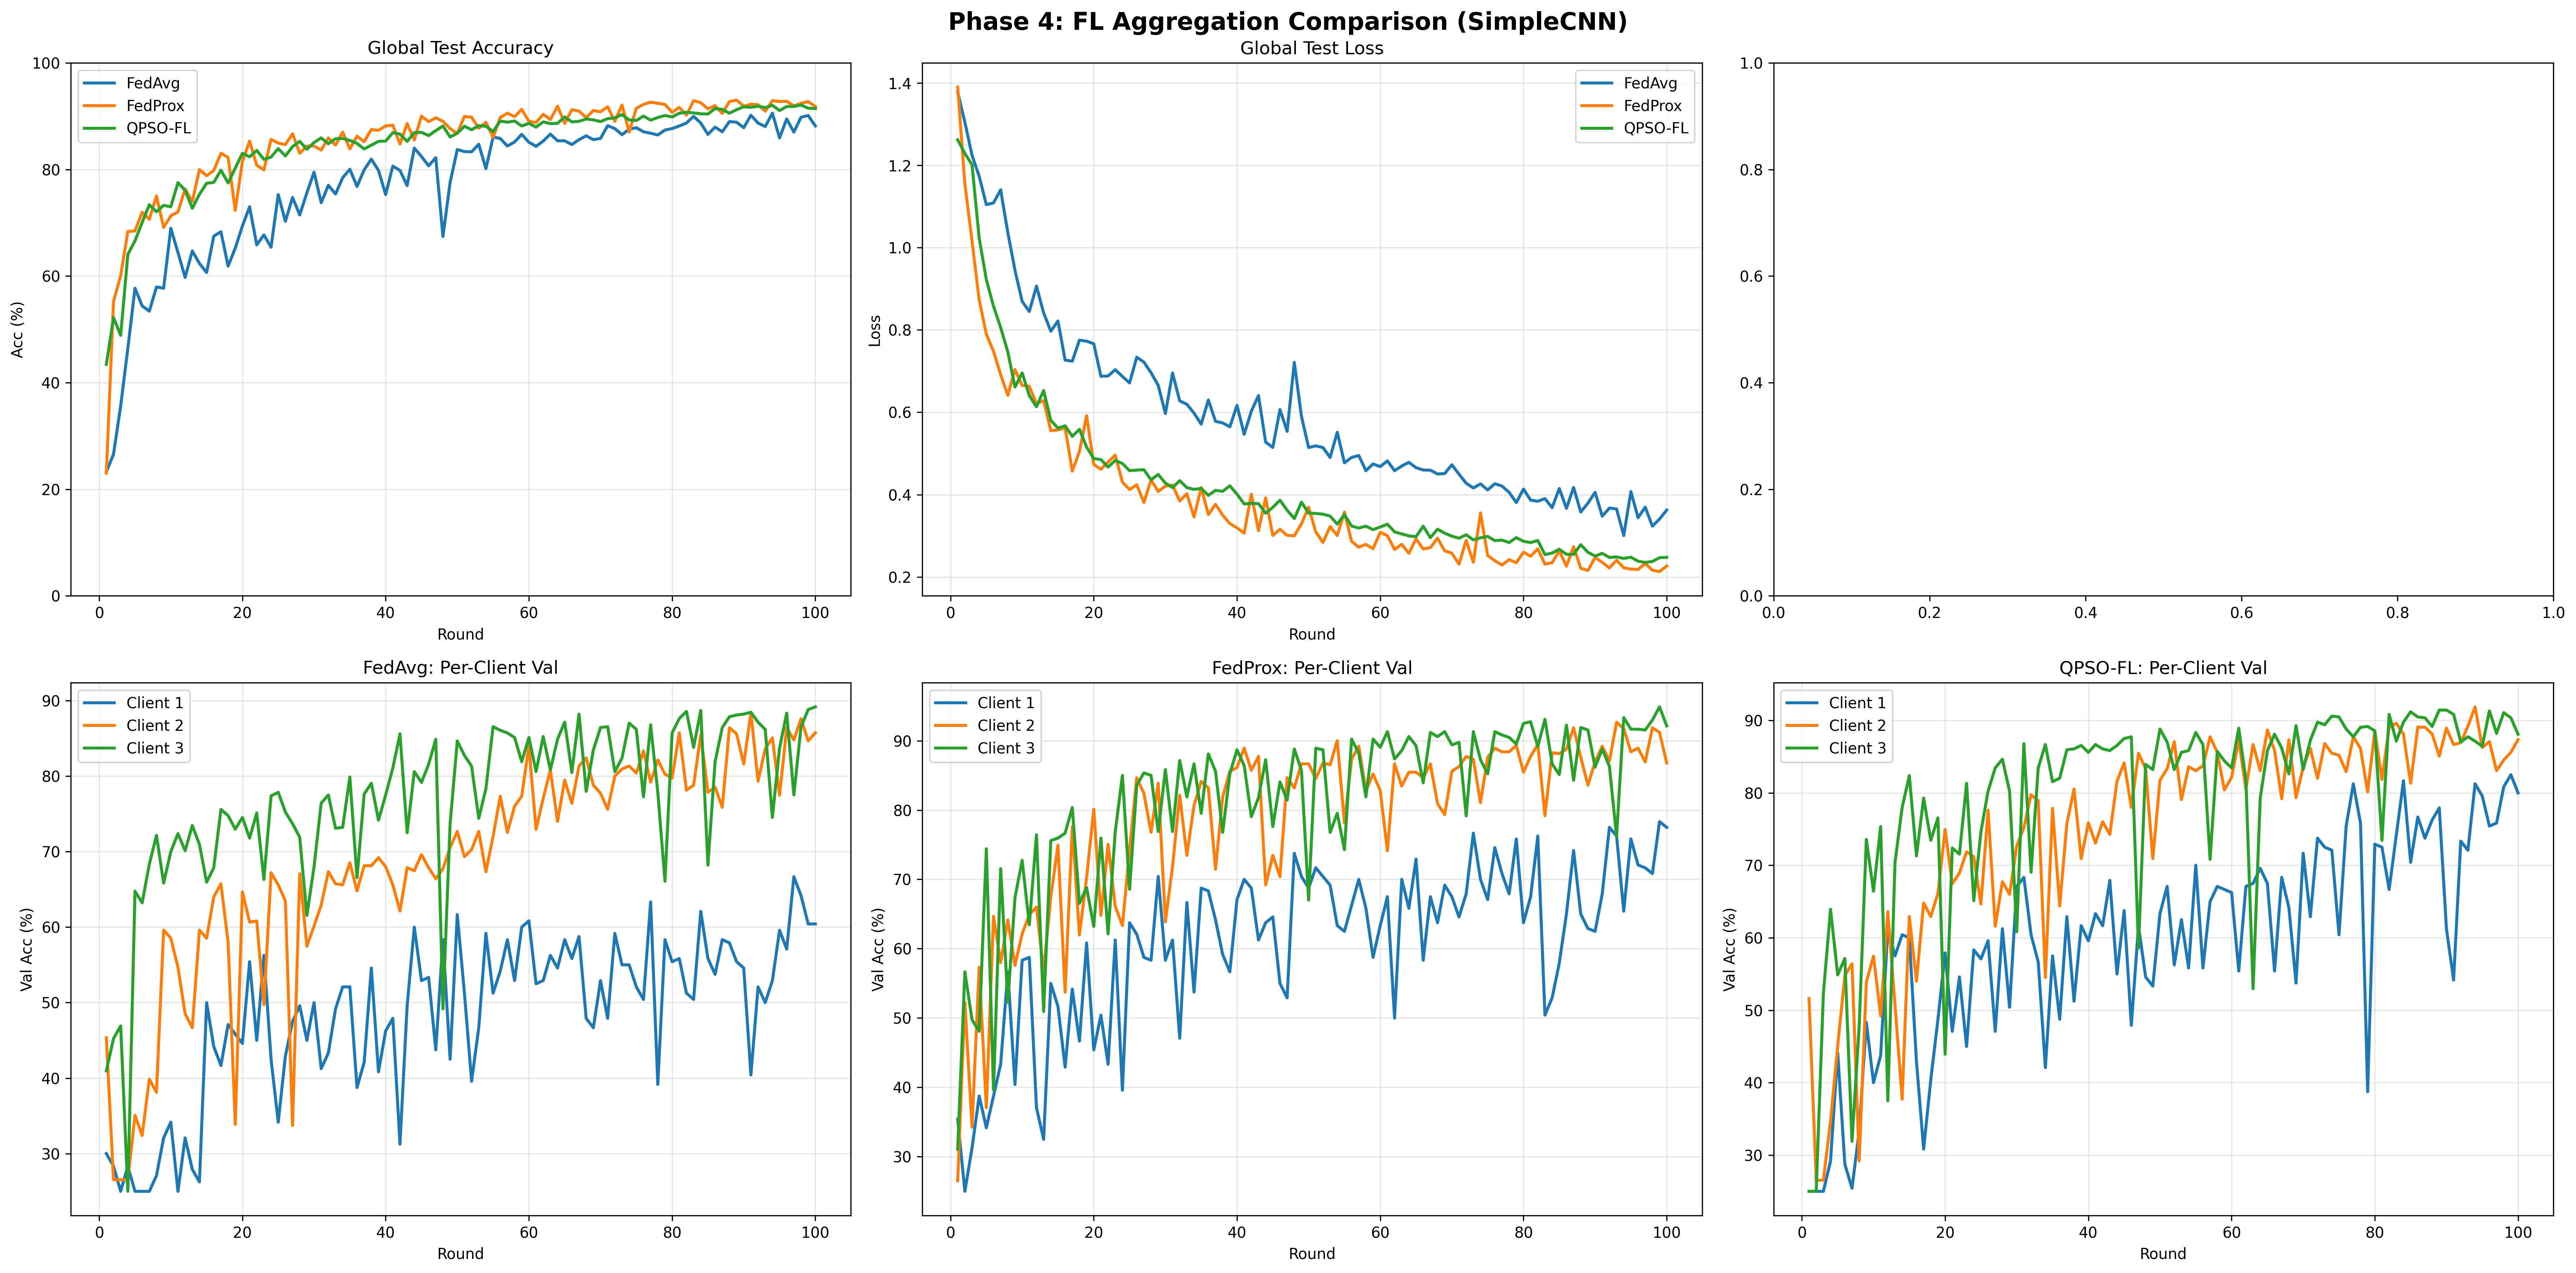
\includegraphics[width=\columnwidth]{s1_comparison.png}}
\caption{Accuracy and loss curves over 100 rounds --- Setup 1 (Natural
Heterogeneity). FedQPSO exhibits markedly lower round-to-round
volatility than FedAvg.}
\label{fig:curves_s1}
\end{figure}

\begin{figure}[t]
\centerline{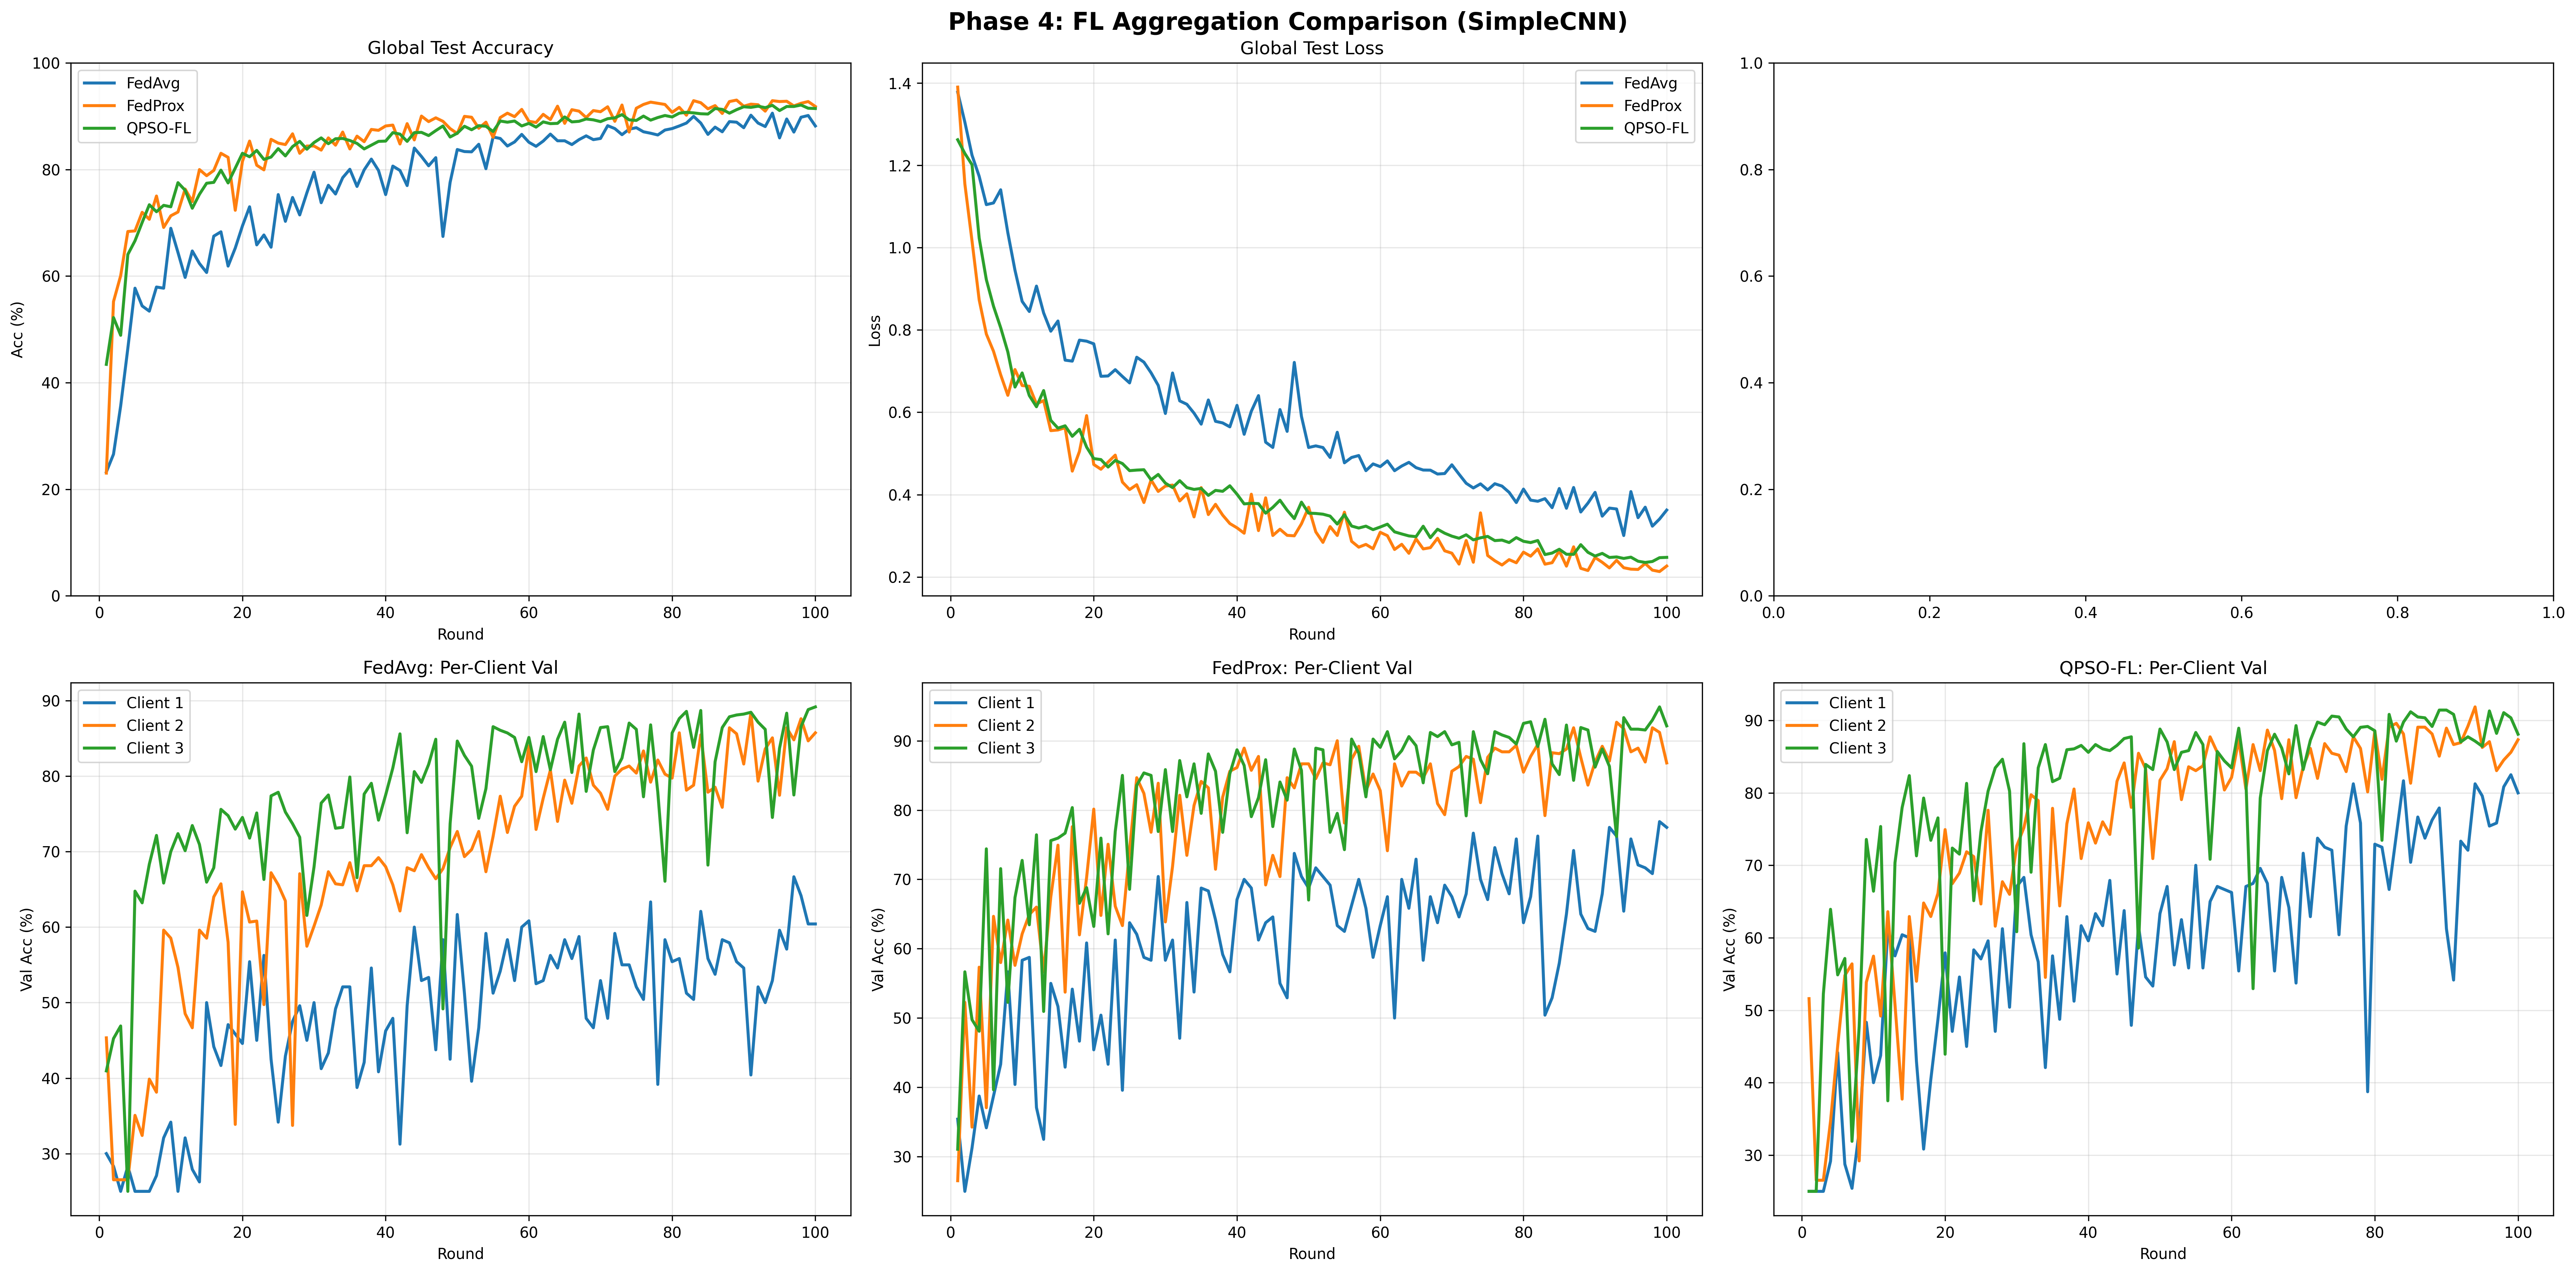
\includegraphics[width=\columnwidth]{s2_comparison.png}}
\caption{Accuracy and loss curves over 100 rounds --- Setup 2 (Moderate Label
Skew). FedAvg degrades significantly faster; FedQPSO shows superior fairness.}
\label{fig:curves_s2}
\end{figure}

\subsection{Per-Class Classification Performance}

Table~\ref{tab:perclass} reports the F1-score and recall for each tumor class
at the respective best-round model checkpoint for each method.

\begin{table}[t]
\caption{Per-Class F1-Score and Recall at Best Model Checkpoint
(S1 = Setup 1, S2 = Setup 2)}
\label{tab:perclass}
\begin{center}
\renewcommand{\arraystretch}{1.15}
\begin{tabular}{llccc}
\hline
\textbf{Setup} & \textbf{Class} & \textbf{FedAvg} & \textbf{FedProx} &
\textbf{FedQPSO}\\
\hline
\multirow{5}{*}{S1 F1}
 & Glioma    & 0.9438 & 0.9420 & \textbf{0.9560}\\
 & Meningioma & 0.9378 & \textbf{0.9394} & 0.9211\\
 & No Tumor  & 0.9663 & \textbf{0.9790} & 0.9602\\
 & Pituitary & 0.9828 & \textbf{0.9846} & 0.9686\\
 & Macro Avg & 0.9577 & \textbf{0.9612} & 0.9515\\
\hline
\multirow{5}{*}{S2 F1}
 & Glioma    & 0.8841 & 0.9039 & \textbf{0.9089}\\
 & Meningioma & 0.8458 & \textbf{0.8921} & 0.8727\\
 & No Tumor  & 0.9447 & \textbf{0.9554} & 0.9528\\
 & Pituitary & 0.9491 & \textbf{0.9689} & 0.9507\\
 & Macro Avg & 0.9059 & \textbf{0.9301} & 0.9213\\
\hline
\multirow{2}{*}{Recall}
 & Glioma (S1) & 0.9118 & 0.9186 & \textbf{0.9593}\\
 & Glioma (S2) & 0.8371 & 0.8620 & \textbf{0.8914}\\
\hline
\end{tabular}
\end{center}
\end{table}

FedQPSO achieves the \textbf{highest Glioma F1 and recall in both setups} --- the
most clinically critical tumor class, where missed diagnoses carry potentially
fatal consequences. Compared to FedAvg under label skew, FedQPSO's Glioma
recall improvement of 5.43 pp corresponds to approximately 24 additional
correctly identified glioma cases per 1,000 patients.

\subsection{Client Fairness --- Primary Finding}

Table~\ref{tab:fairness} presents client fairness metrics. Fig.~\ref{fig:fairness_s1}
and Fig.~\ref{fig:fairness_s2} visualize per-client accuracy distributions.

\begin{table}[t]
\caption{Client Fairness Metrics (Final Round and At-Peak-Round)}
\label{tab:fairness}
\begin{center}
\renewcommand{\arraystretch}{1.15}
\begin{tabular}{llccc}
\hline
\textbf{Setup} & \textbf{Metric} & \textbf{FedAvg} & \textbf{FedProx} &
\textbf{FedQPSO}\\
\hline
\multirow{4}{*}{S1}
 & Cl.\ 1 final (\%) & 83.75 & 91.25 & \textbf{92.08}\\
 & Client $\sigma$ final & 5.28\% & 2.27\% & \textbf{1.56\%}\\
 & Max$-$Min gap (pp) & 12.20 & 5.30 & \textbf{2.32}\\
 & Client $\sigma$ at peak & 9.50\% & 2.79\% & \textbf{1.62\%}\\
\hline
\multirow{4}{*}{S2}
 & Cl.\ 1 final (\%) & 60.42 & 77.50 & \textbf{80.00}\\
 & Client $\sigma$ final & 12.82\% & 6.05\% & \textbf{3.65\%}\\
 & Max$-$Min gap (pp) & 28.75 & 14.64 & \textbf{8.10}\\
 & Client $\sigma$ at peak & 13.38\% & 12.07\% & \textbf{4.23\%}\\
\hline
\end{tabular}
\end{center}
\end{table}

\begin{figure}[t]
\centerline{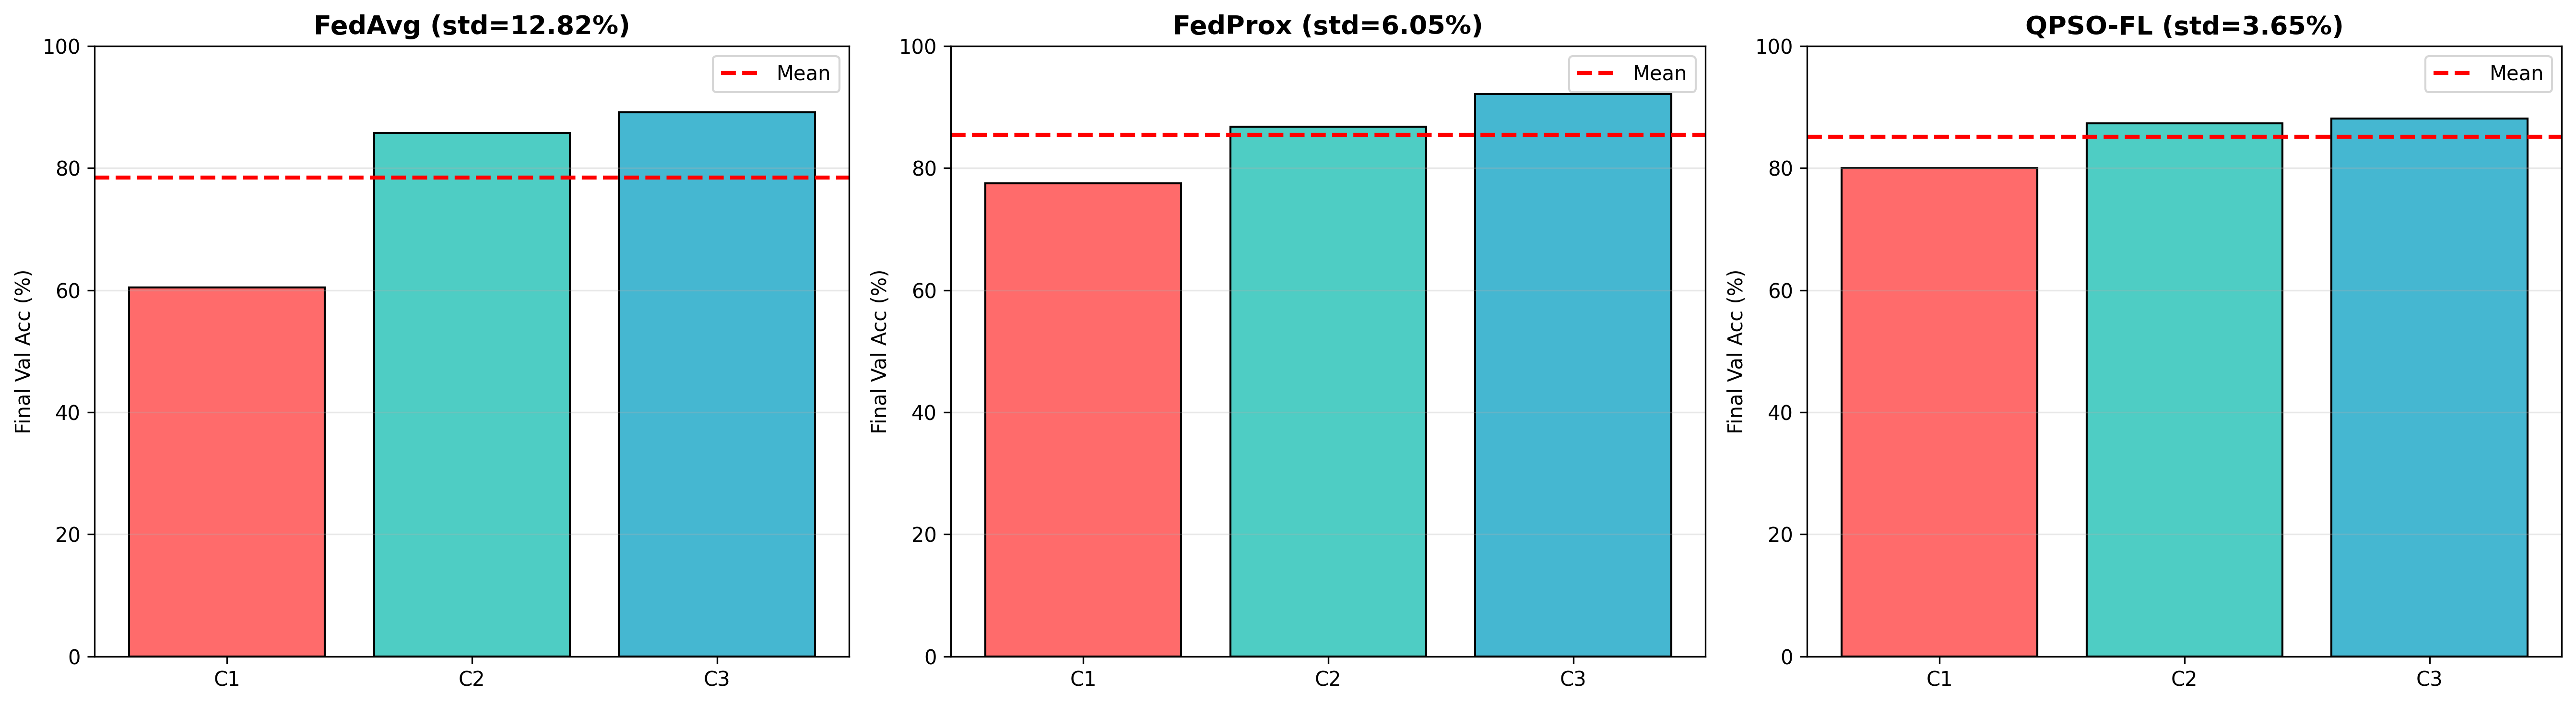
\includegraphics[width=\columnwidth]{s1_fairness.png}}
\caption{Per-client validation accuracy --- Setup 1. When FedAvg peaks
globally at 95.80\%, Client 1 is simultaneously at 75.00\% --- a 20 pp
inequity hidden by the global metric. FedQPSO keeps all clients within 3.5 pp.}
\label{fig:fairness_s1}
\end{figure}

\begin{figure}[t]
\centerline{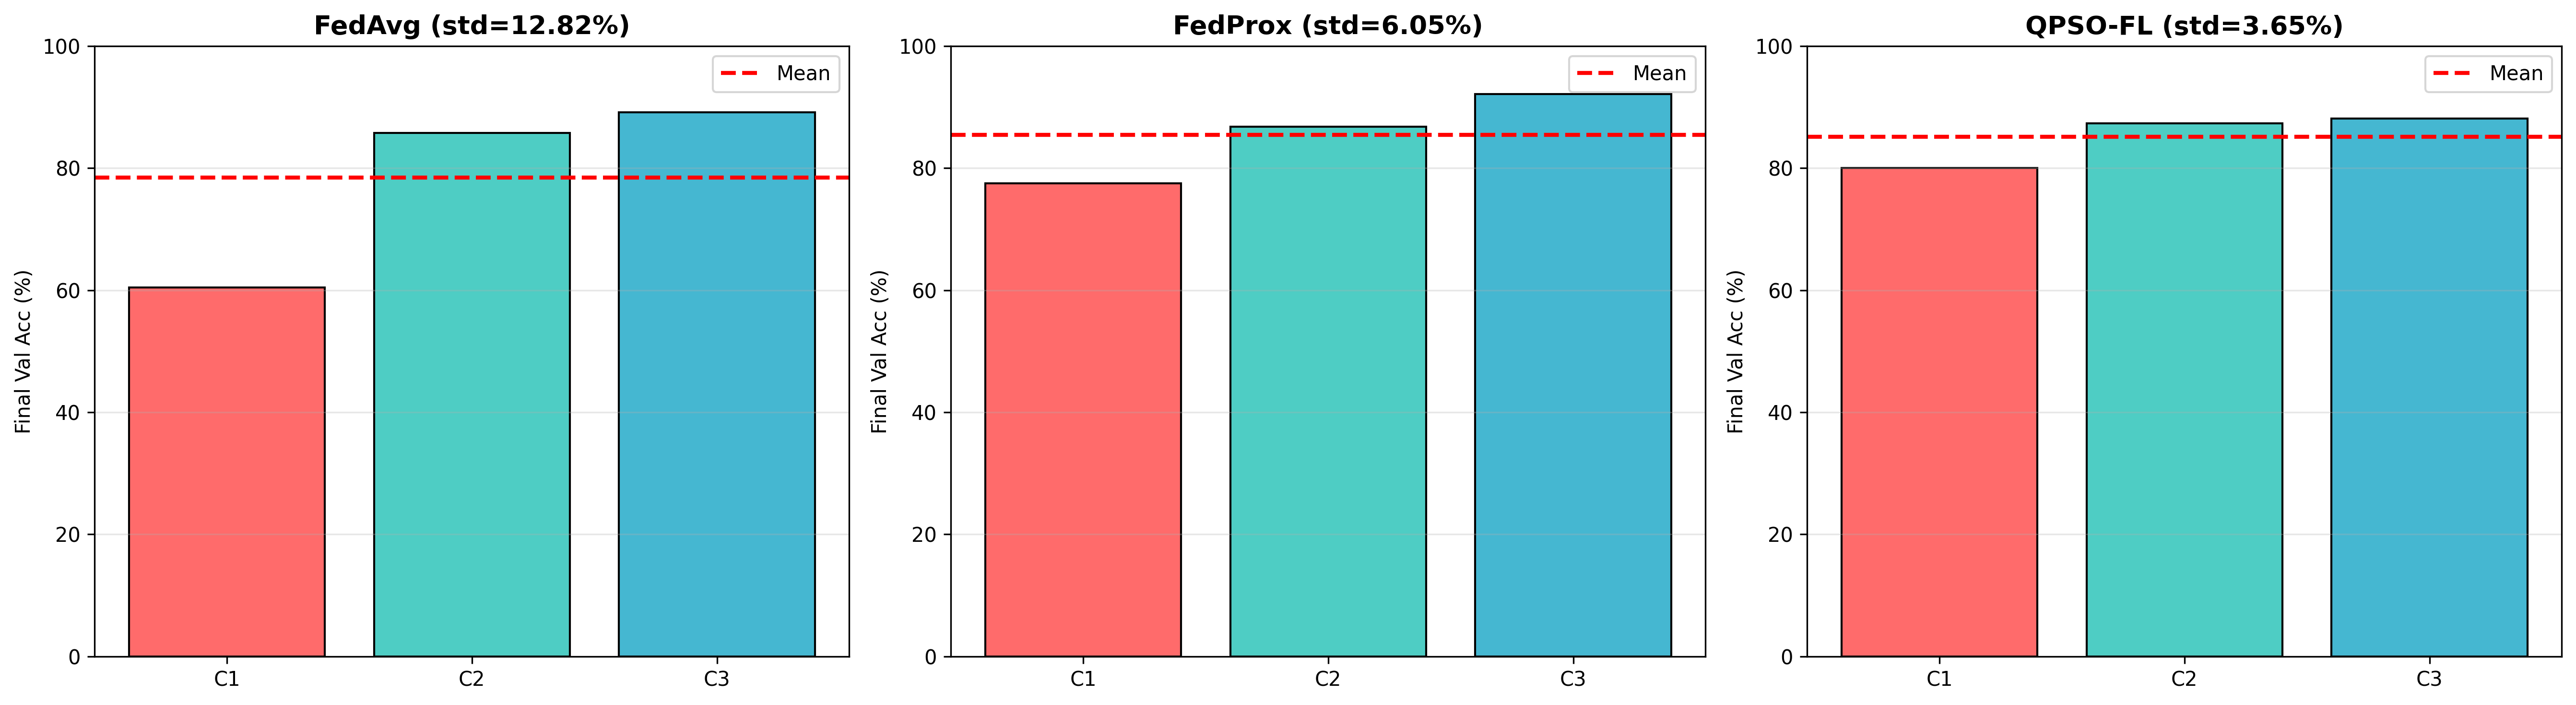
\includegraphics[width=\columnwidth]{s2_fairness.png}}
\caption{Per-client validation accuracy --- Setup 2 (label skew). Under
FedAvg, Client 1 never exceeds 70\% in any of 100 rounds. FedQPSO is
the only method keeping Client 1 above 80\% at convergence.}
\label{fig:fairness_s2}
\end{figure}

The most clinically significant result: at FedAvg's peak global accuracy of
90.56\% (Setup 2), Client~1's validation accuracy was simultaneously
\textbf{52.92\%} --- barely above random chance for a 4-class problem. At
FedQPSO's peak (92.09\%), Client~1 was at \textbf{80.83\%} --- a 27.91 pp
improvement for the weakest hospital at the same moment of best global
performance.

FedQPSO reduces FedAvg's max-min client accuracy gap by \textbf{81\%} in
Setup 1 (12.20 $\to$ 2.32 pp) and \textbf{72\%} in Setup 2 (28.75 $\to$
8.10 pp), and exceeds FedProx by 45--56\% on the same metric. Critically, the
QPSO--FedProx fairness gap \emph{widens} from 0.71 pp to 2.40 pp in client
$\sigma$ as heterogeneity increases --- the mechanism becomes more effective
under harder conditions.

\subsection{Statistical Significance}

Results of paired two-tailed $t$-tests on per-round global accuracy sequences
are summarized in Table~\ref{tab:stats}.

\begin{table}[t]
\caption{Statistical Significance: Paired $t$-Test on Per-Round Accuracy}
\label{tab:stats}
\begin{center}
\begin{tabular}{llcccl}
\hline
\textbf{Setup} & \textbf{Comparison} & $t$ & $p$ & $d$ & \textbf{Sig.}\\
\hline
S1 & FedAvg vs FedQPSO  & 3.43 & 0.000882 & 0.35 & \checkmark \\
S1 & FedAvg vs FedProx  & 1.72 & 0.0879   & 0.17 & $\times$ \\
S2 & FedAvg vs FedQPSO  & 12.59 & $2.91\!\times\!10^{-22}$ & 1.26 & \checkmark \\
S2 & FedAvg vs FedProx  & 13.39 & $5.86\!\times\!10^{-24}$ & 1.34 & \checkmark \\
\hline
\multicolumn{6}{l}{\small \checkmark: $p < 0.05$; \quad $d$: Cohen's $d$ effect size.}
\end{tabular}
\end{center}
\end{table}

Under natural heterogeneity, \textbf{FedQPSO is the only method that
statistically significantly outperforms FedAvg} ($p = 0.000882$). FedProx
fails to reach significance ($p = 0.088$) --- its proximal term is
insufficient when data distributions are only mildly heterogeneous. Under
label skew, both FedQPSO and FedProx achieve overwhelming statistical
separation from FedAvg (Cohen's $d > 1.2$ for both, representing a large
effect). The jump in Cohen's $d$ from 0.35 (Setup 1) to 1.26 (Setup 2)
confirms that FedQPSO's advantage scales with heterogeneity severity.

\subsection{ROC-AUC Analysis}

\begin{table}[t]
\caption{ROC-AUC Per Class and Micro Average}
\label{tab:auc}
\begin{center}
\begin{tabular}{lcccc}
\hline
& \multicolumn{3}{c}{\textbf{Setup 1}} &
  \multicolumn{3}{c}{\textbf{Setup 2}}\\
\cmidrule(lr){2-4}\cmidrule(lr){5-7}
\textbf{Class} & FA & FP & \textbf{FQ} & FA & FP & \textbf{FQ}\\
\hline
Glioma      & 0.988 & 0.988 & \textbf{0.991} & 0.977 & 0.983 & \textbf{0.985}\\
Meningioma  & 0.992 & \textbf{0.993} & 0.986 & 0.970 & \textbf{0.981} & 0.978\\
No Tumor    & 0.998 & \textbf{0.999} & 0.995 & 0.996 & \textbf{0.997} & \textbf{0.997}\\
Pituitary   & \textbf{0.999} & \textbf{0.999} & 0.998 & 0.996 & \textbf{0.997} & \textbf{0.997}\\
Micro Avg   & 0.995 & \textbf{0.996} & 0.993 & 0.986 & \textbf{0.991} & 0.990\\
\hline
\multicolumn{7}{l}{\small FA=FedAvg, FP=FedProx, FQ=FedQPSO.}
\end{tabular}
\end{center}
\end{table}

All three methods achieve clinically excellent AUC (Table~\ref{tab:auc})
across all classes in both setups --- no AUC falls below 0.970. FedQPSO wins
Glioma AUC in \emph{both} setups (0.991 and 0.985). ROC-AUC curves are shown
in Figs.~\ref{fig:roc_s1} and~\ref{fig:roc_s2}.

\begin{figure}[t]
\centerline{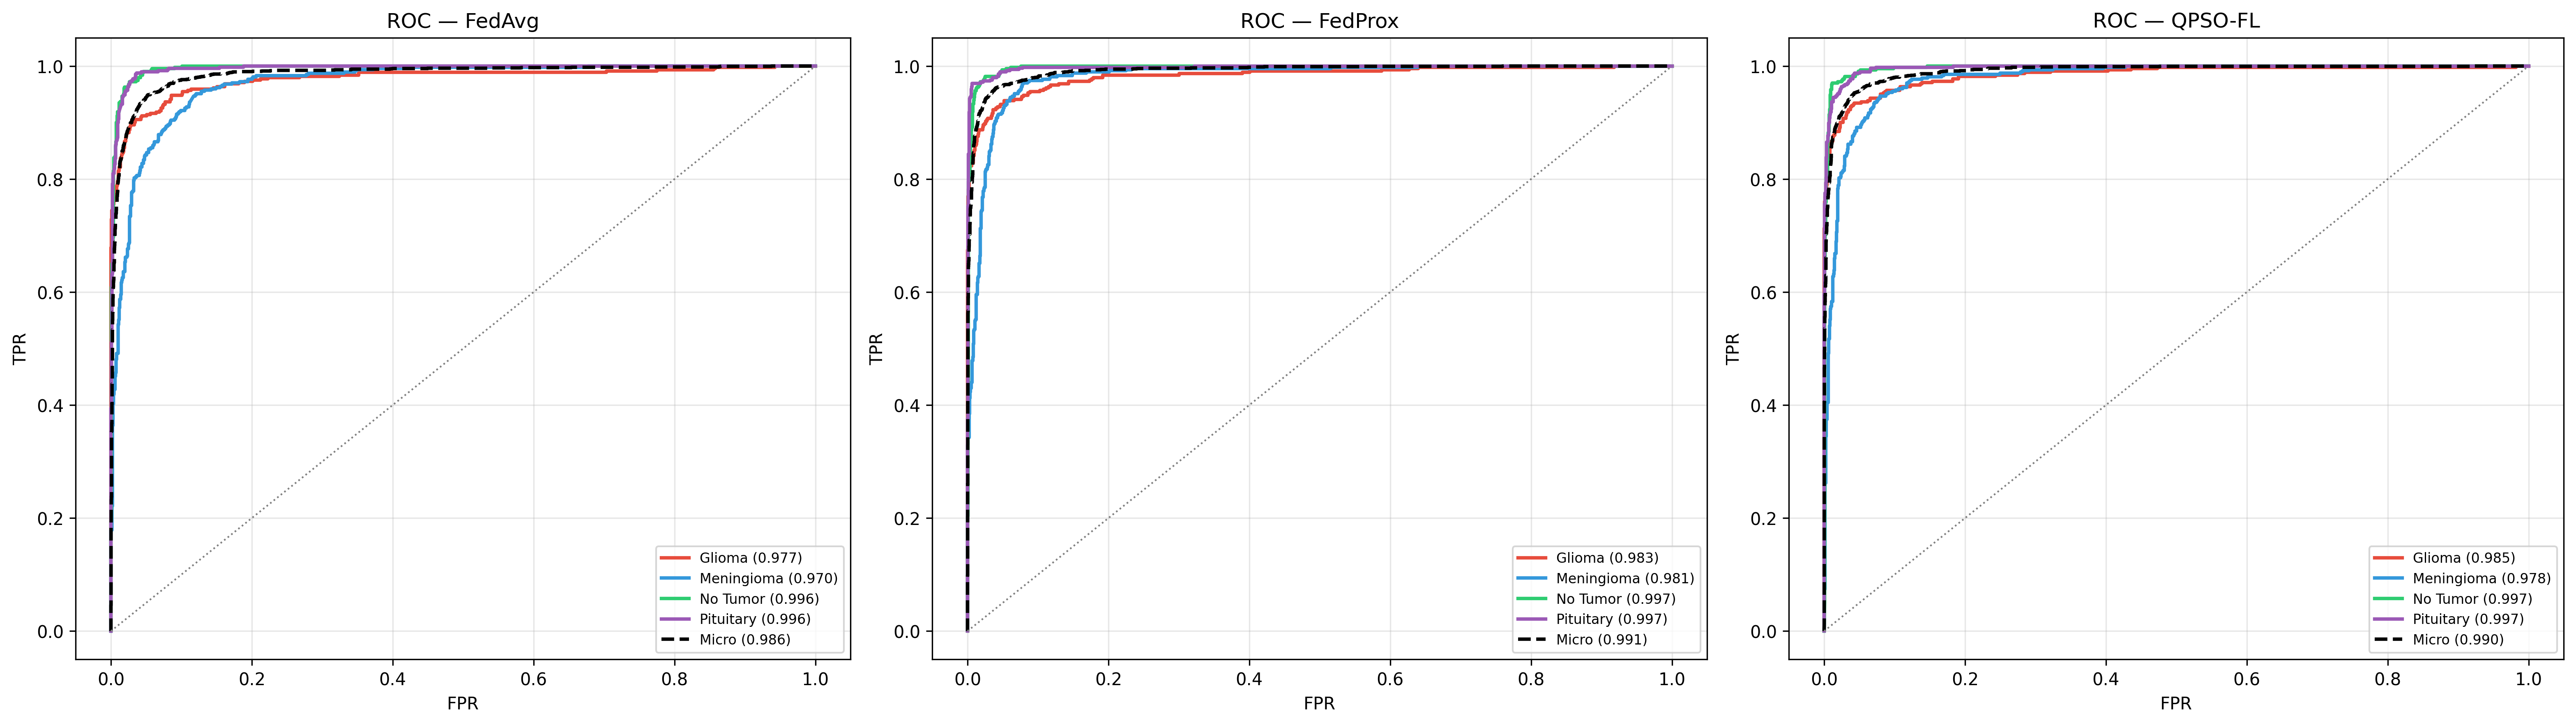
\includegraphics[width=\columnwidth]{s1_roc_auc.png}}
\caption{ROC-AUC curves --- Setup 1. All methods achieve AUC $>$ 0.986 for
every class. FedQPSO leads on the Glioma curve (AUC = 0.991).}
\label{fig:roc_s1}
\end{figure}

\begin{figure}[t]
\centerline{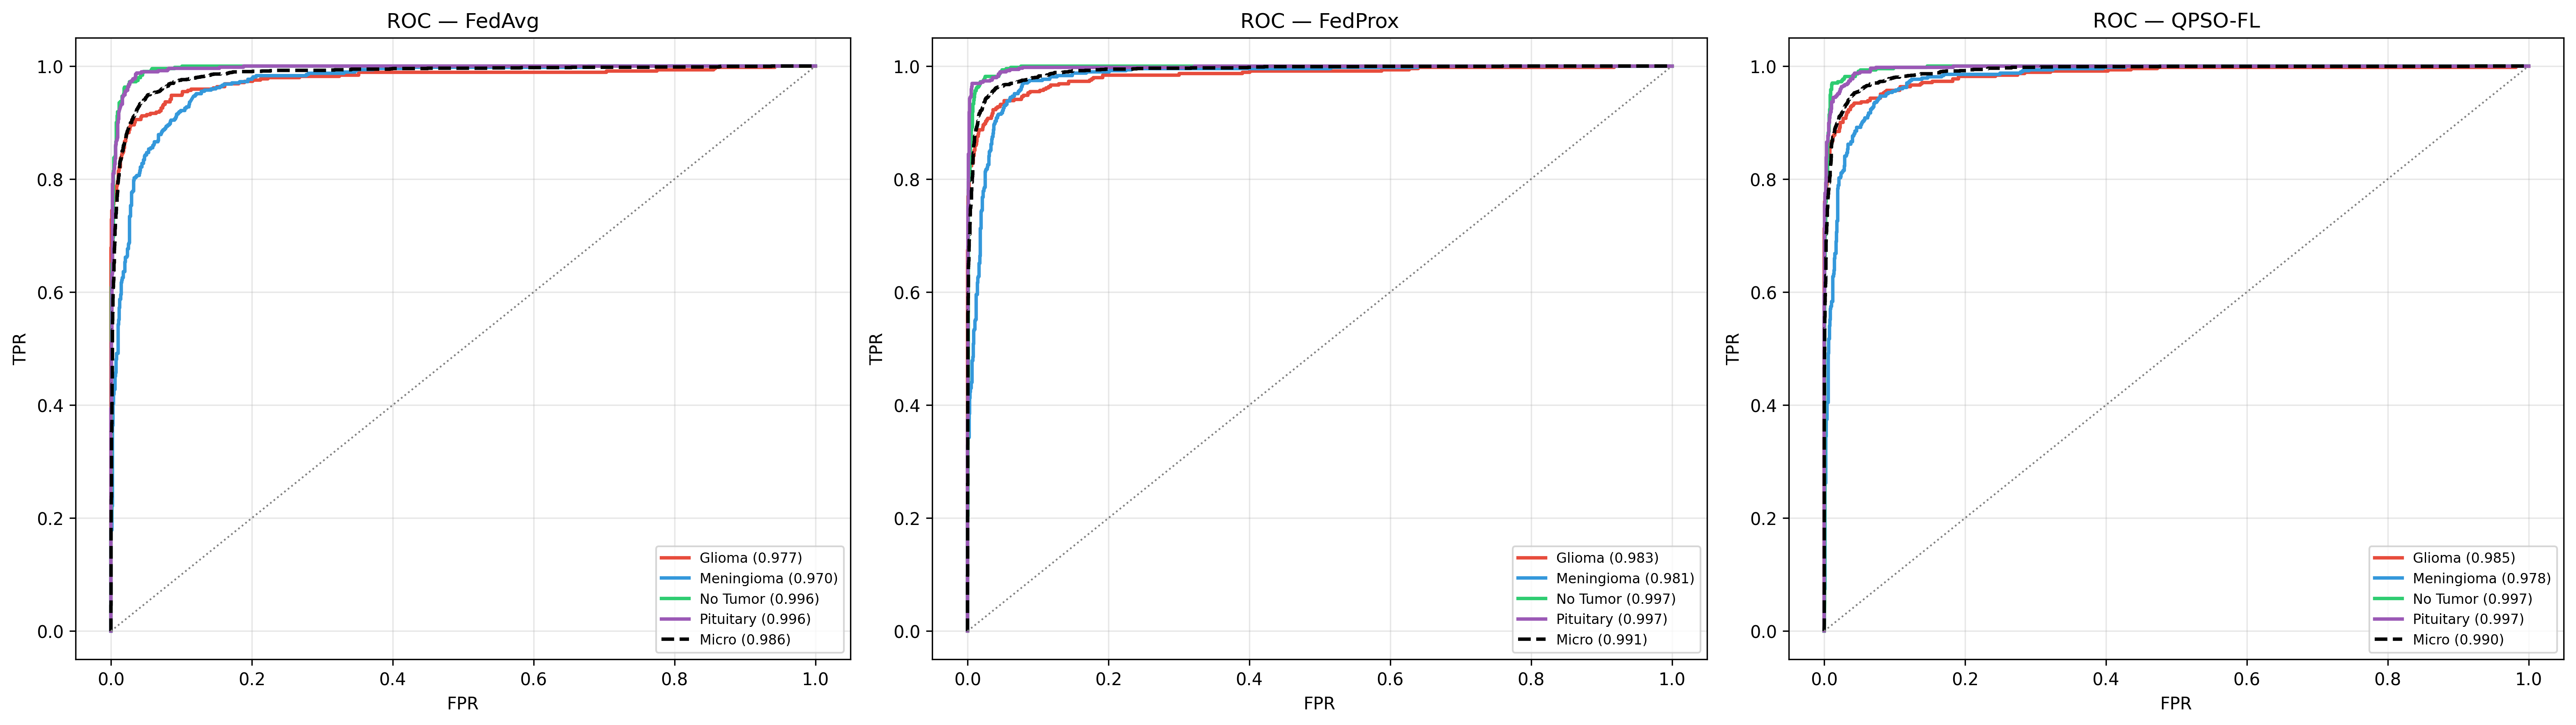
\includegraphics[width=\columnwidth]{s2_roc_auc.png}}
\caption{ROC-AUC curves --- Setup 2. FedAvg Meningioma AUC drops to 0.970
under label skew; FedQPSO maintains above 0.978.}
\label{fig:roc_s2}
\end{figure}

\subsection{Confusion Matrices}

Figs.~\ref{fig:cm_s1} and~\ref{fig:cm_s2} show the confusion matrices for
all three methods at their best-round checkpoints.

\begin{figure}[t]
\centerline{%
  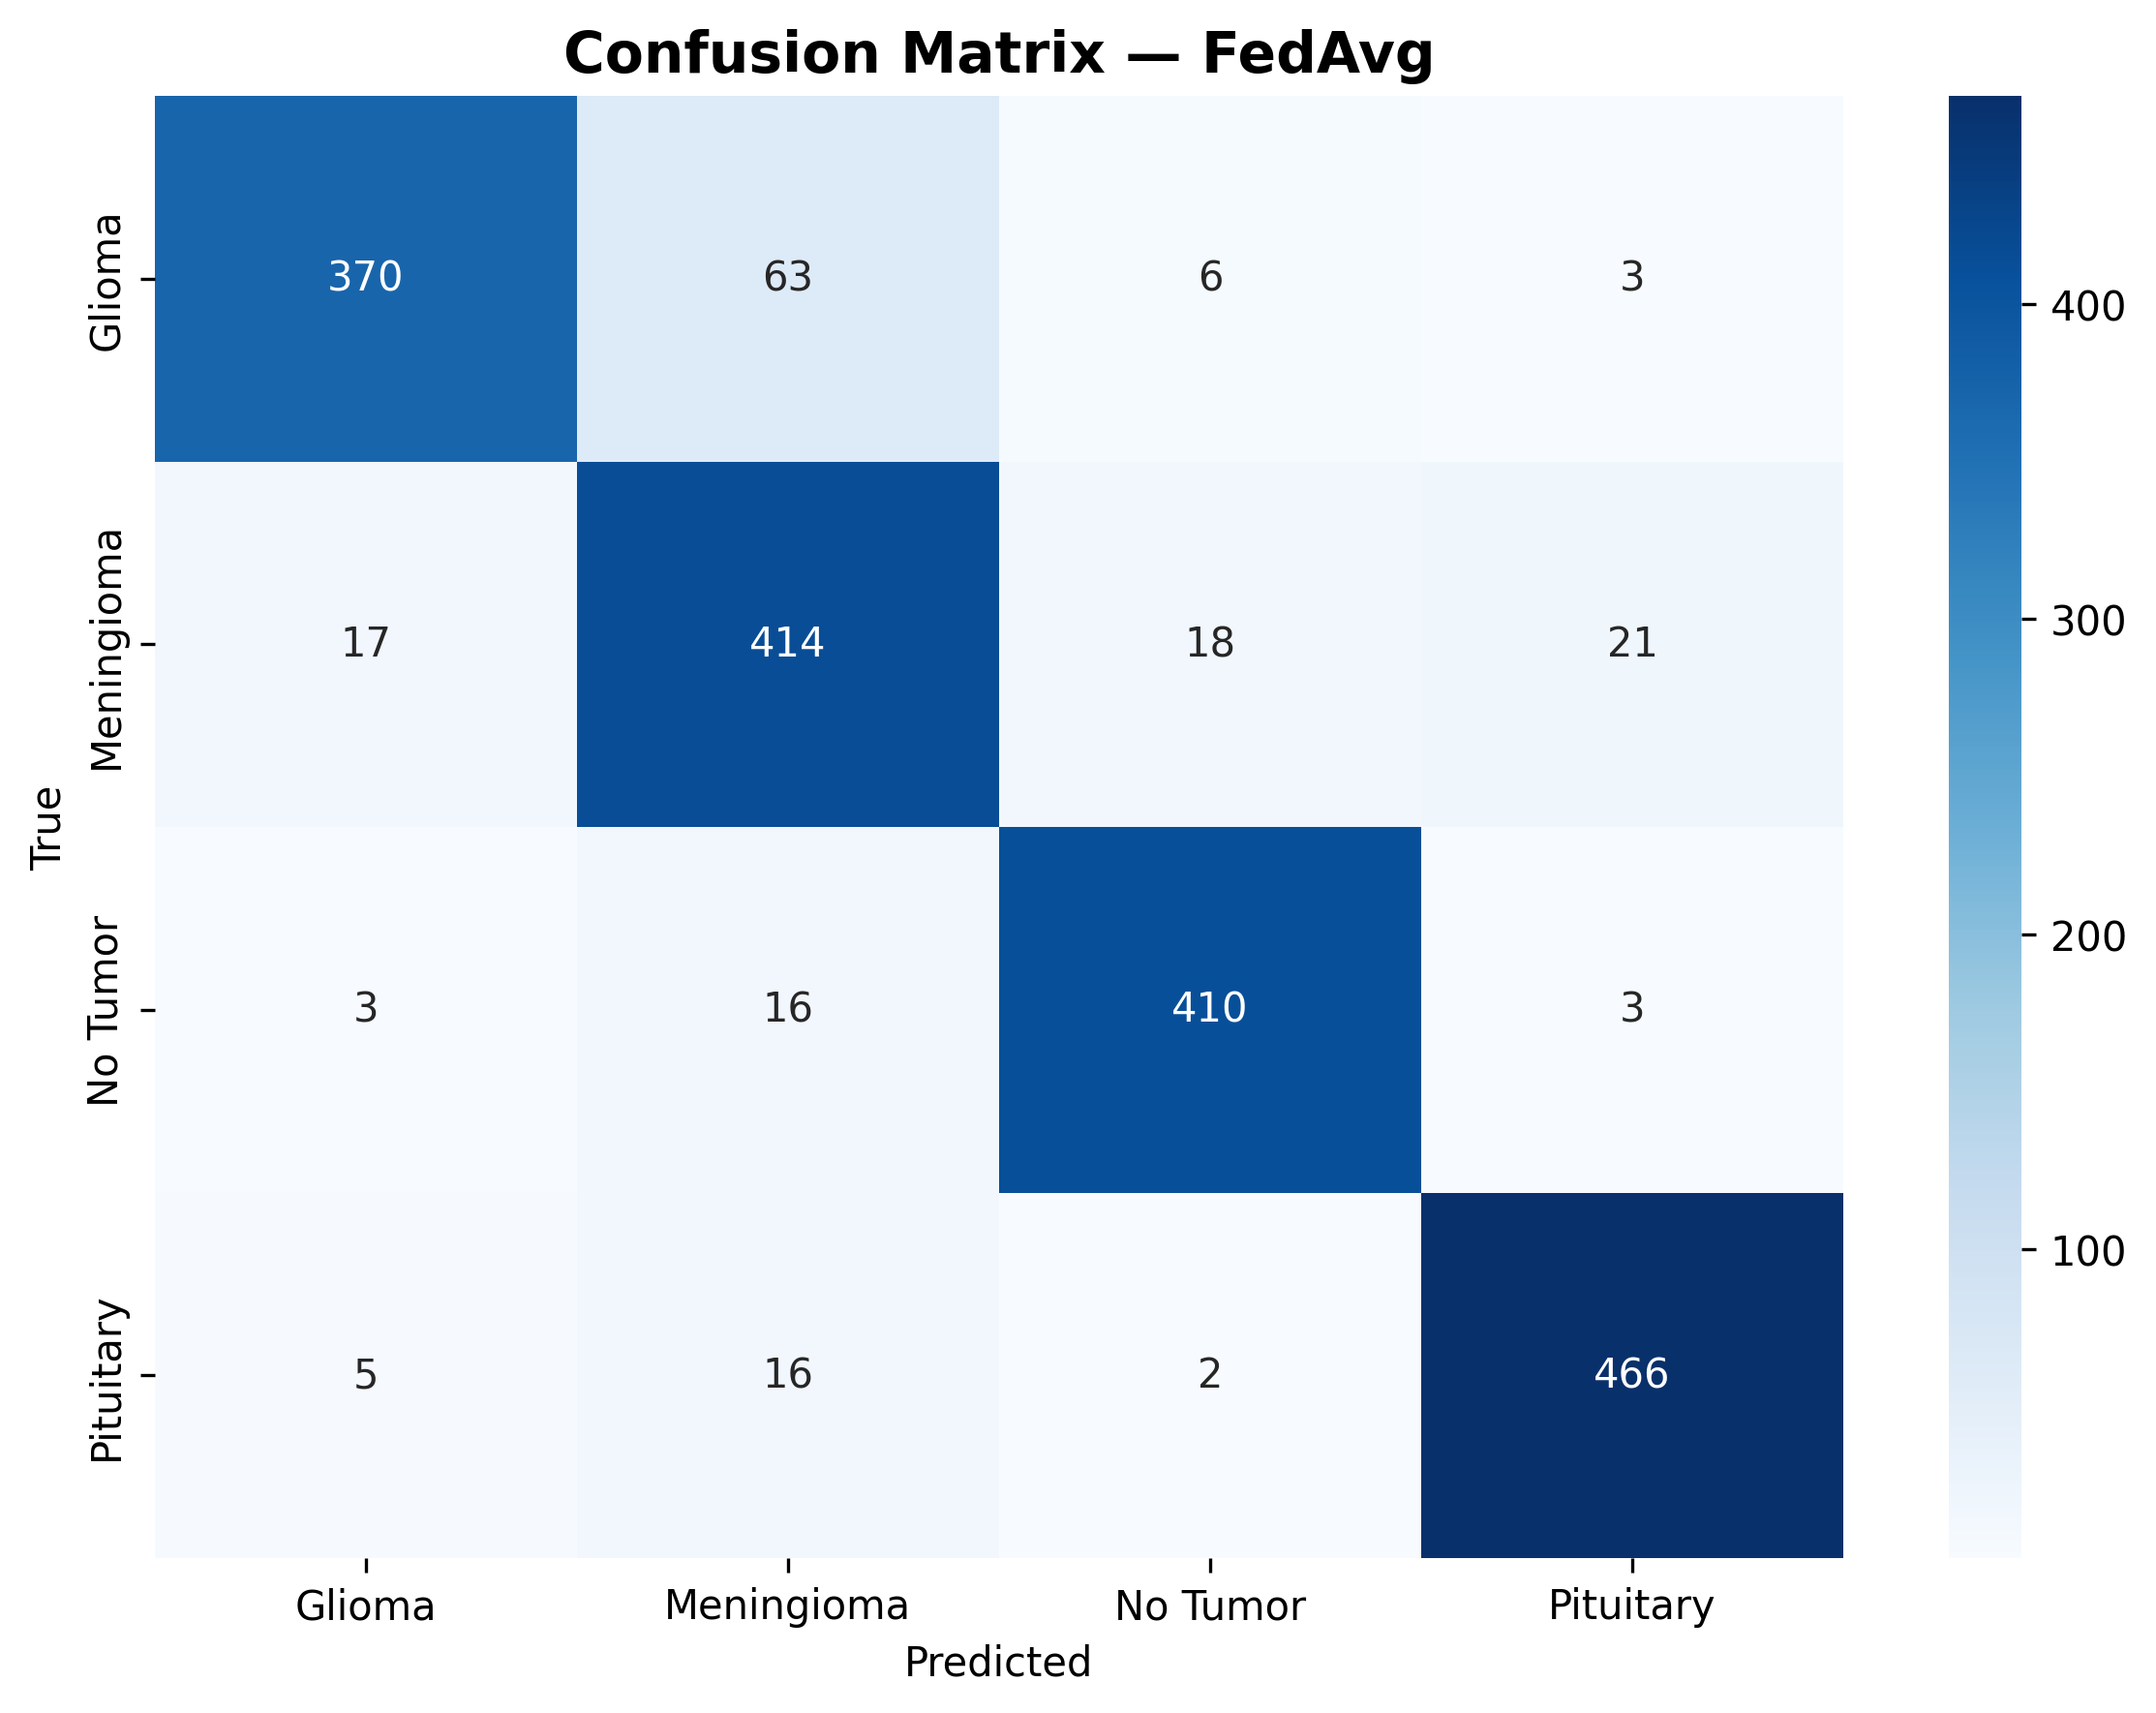
\includegraphics[width=0.48\columnwidth]{s1_cm_fedavg.png}%
  \hfill
  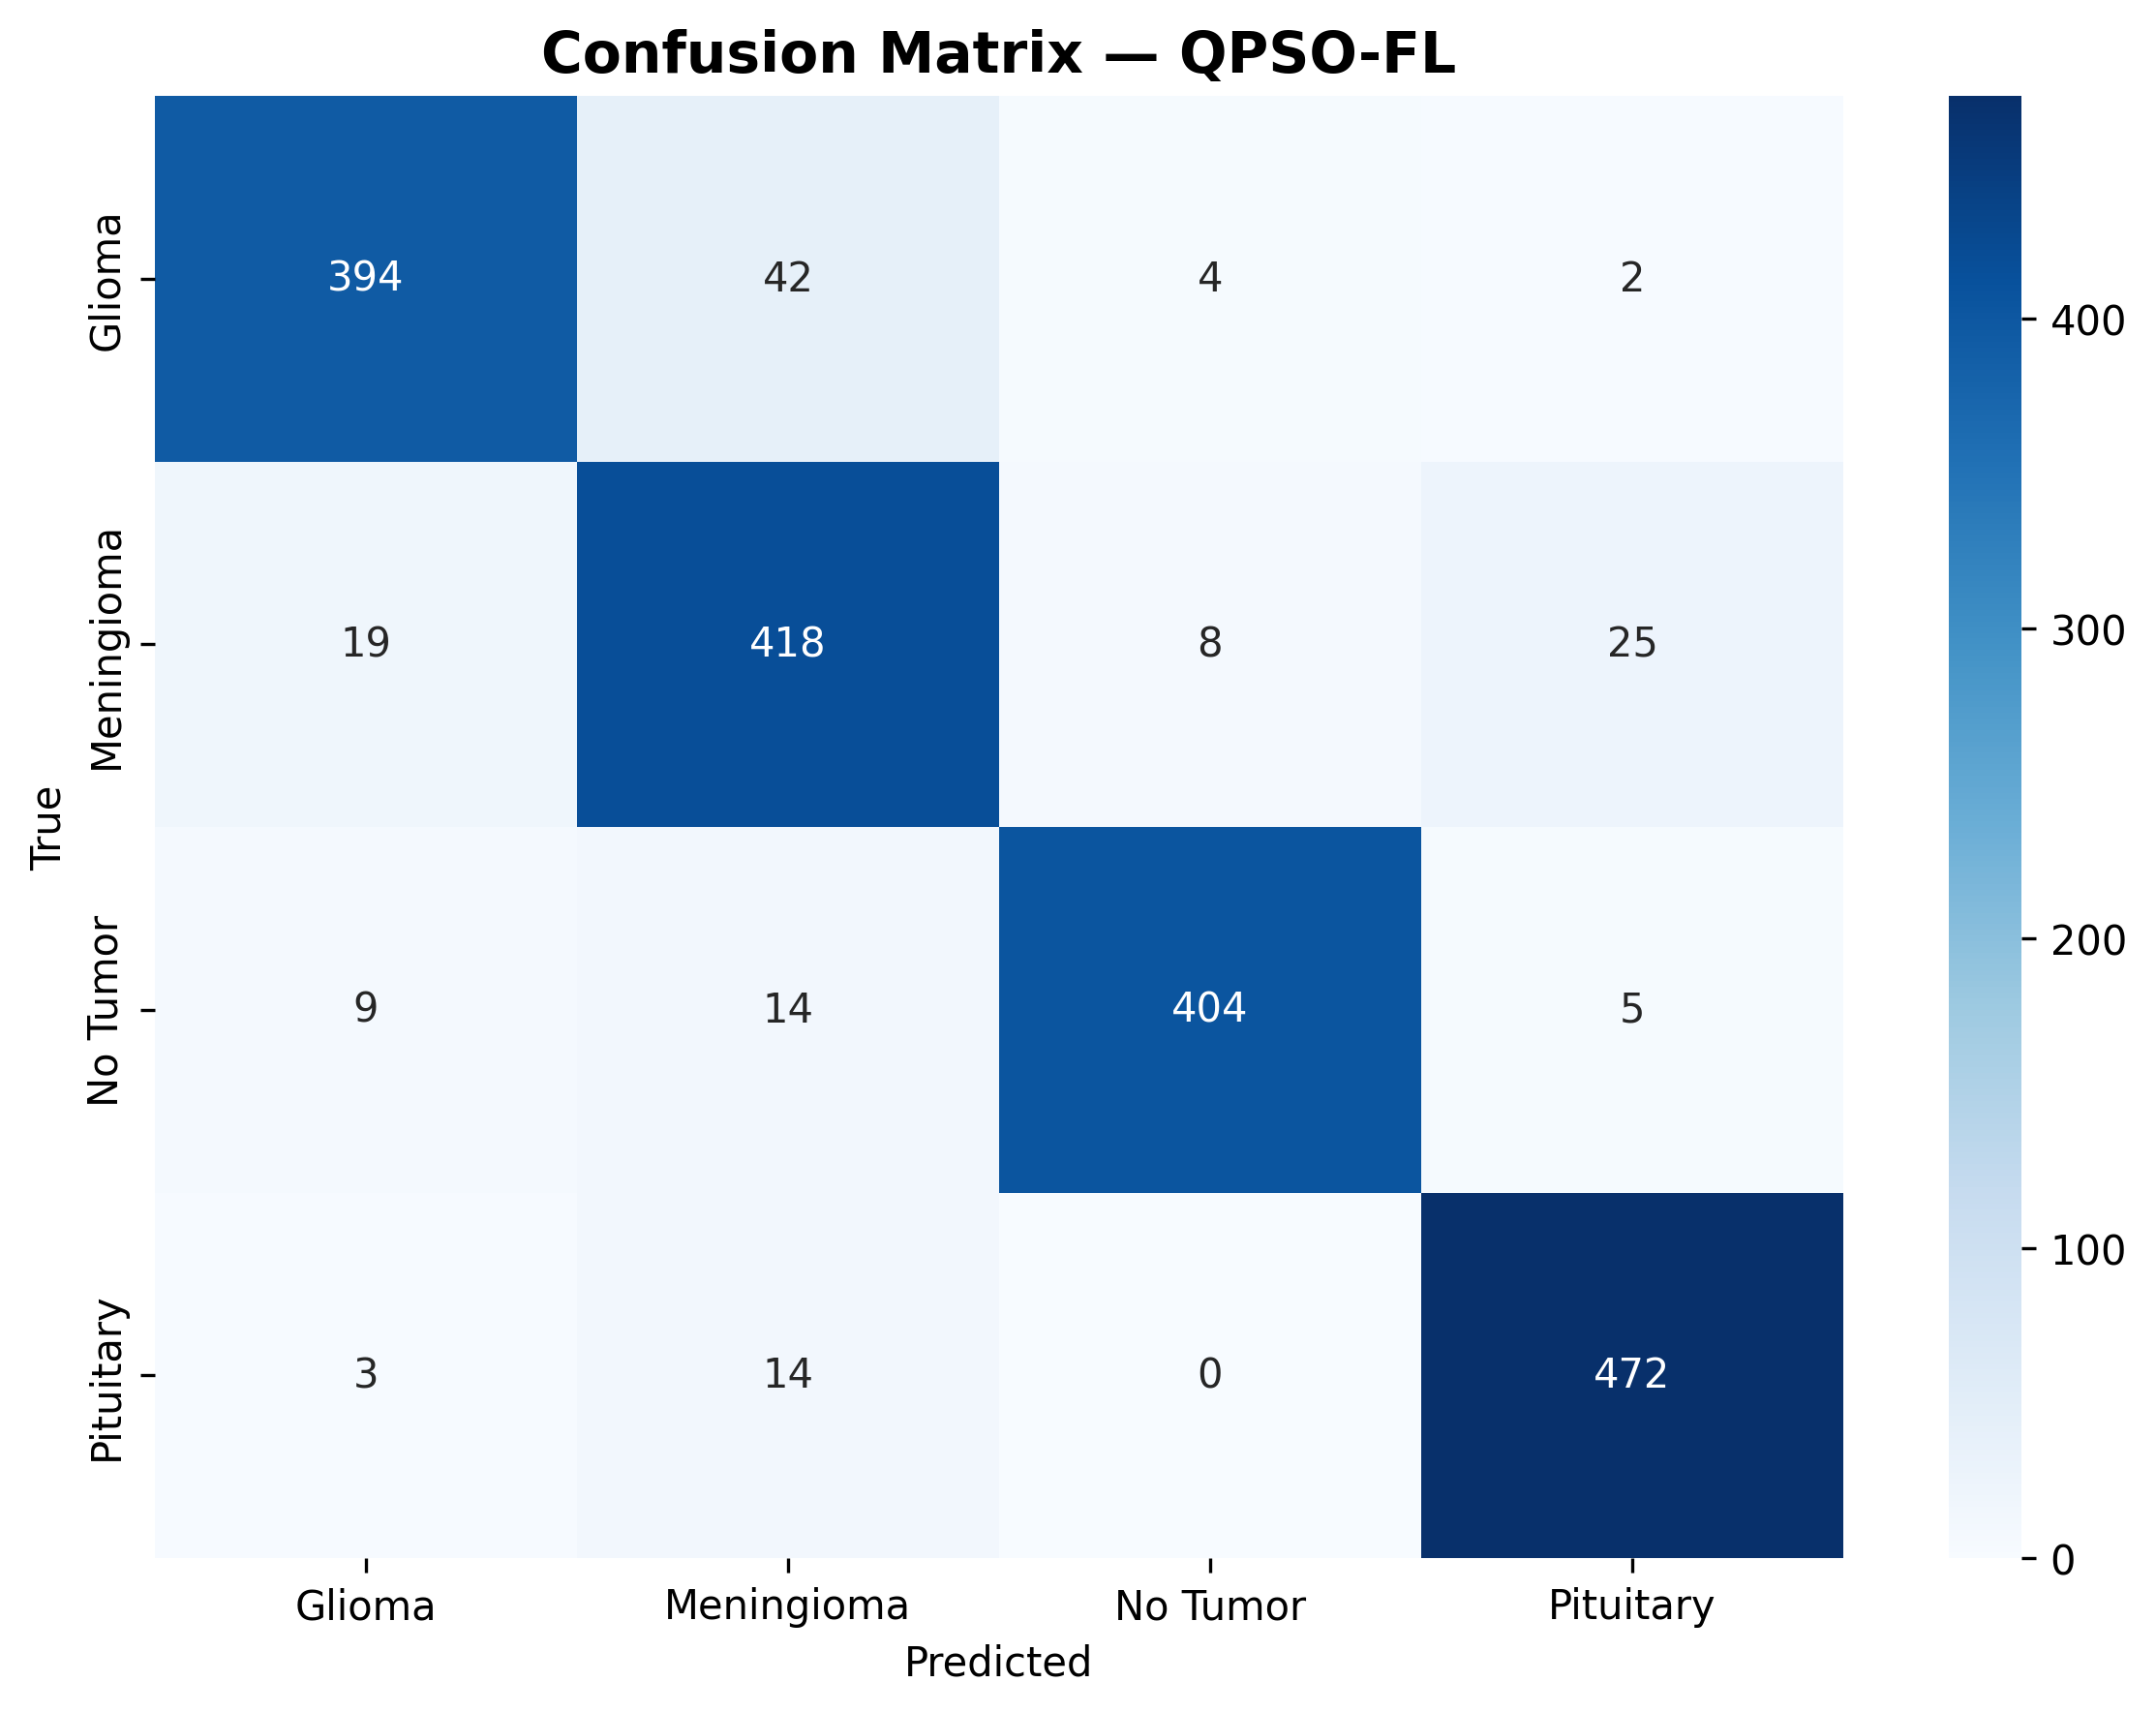
\includegraphics[width=0.48\columnwidth]{s1_cm_qpso.png}}
\caption{Confusion matrices --- Setup 1. Left: FedAvg. Right: FedQPSO. FedQPSO shows fewer Glioma misclassifications.}
\label{fig:cm_s1}
\end{figure}

\begin{figure}[t]
\centerline{%
  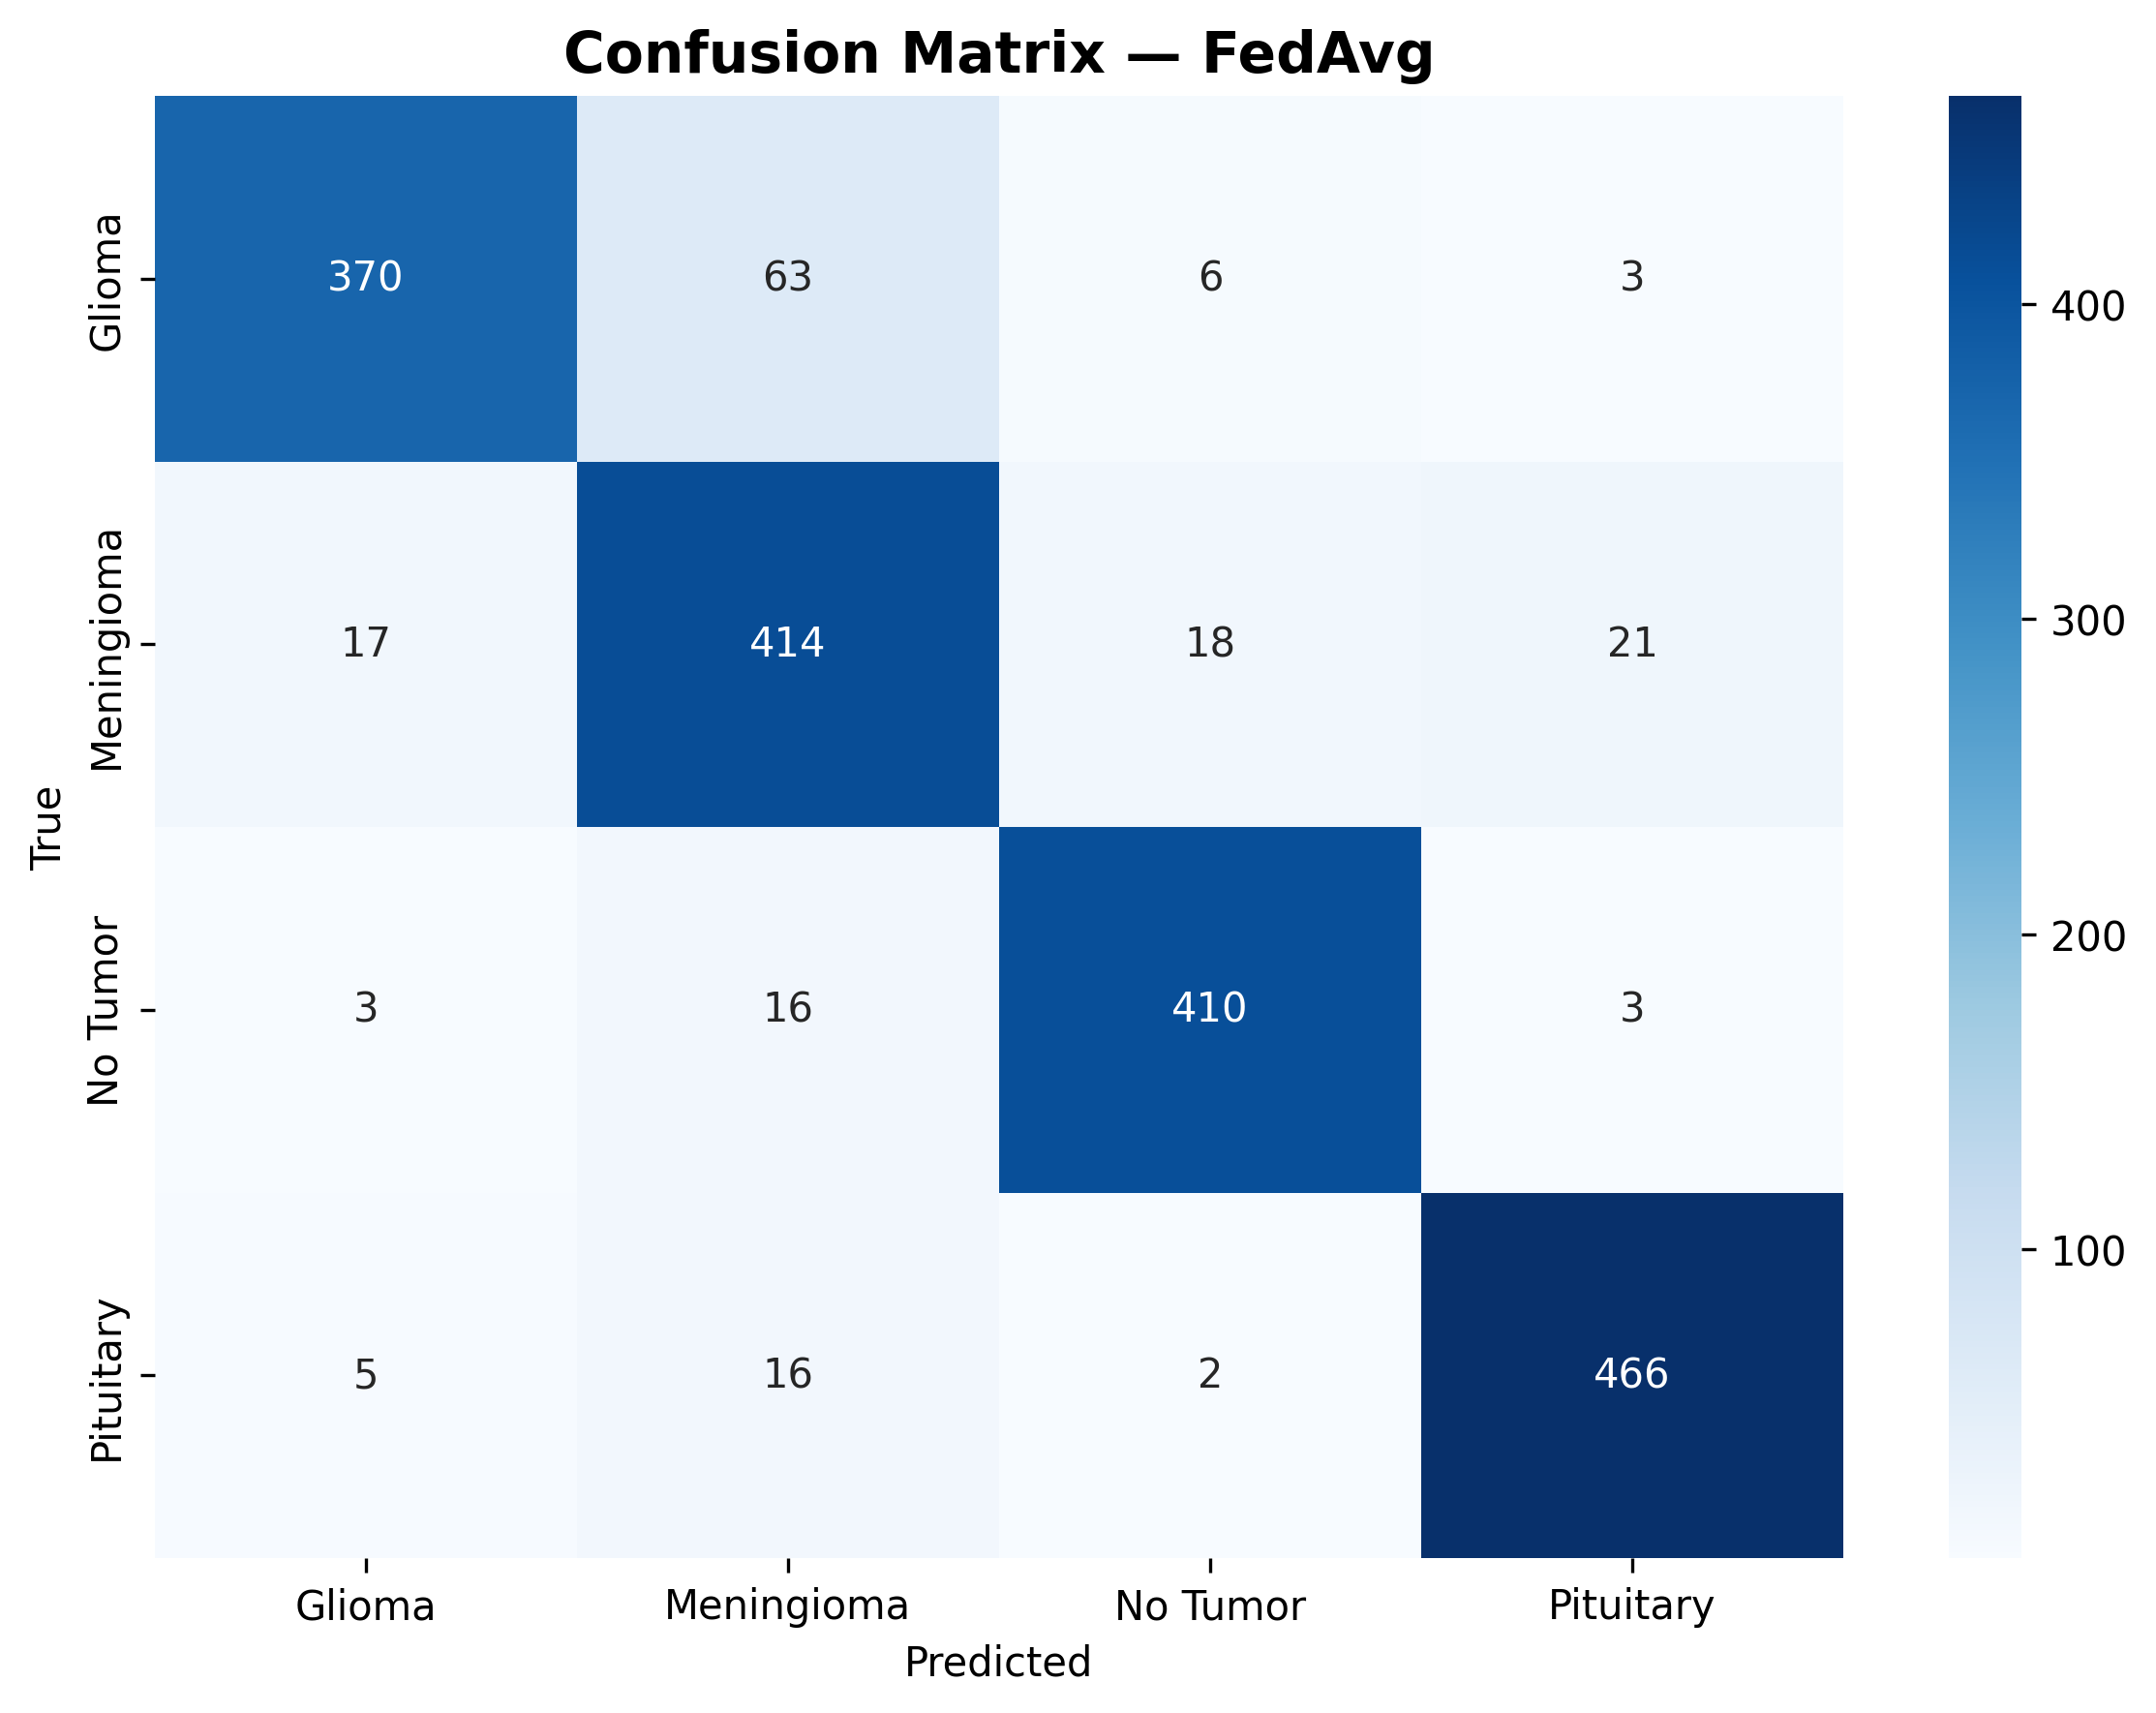
\includegraphics[width=0.48\columnwidth]{s2_cm_fedavg.png}%
  \hfill
  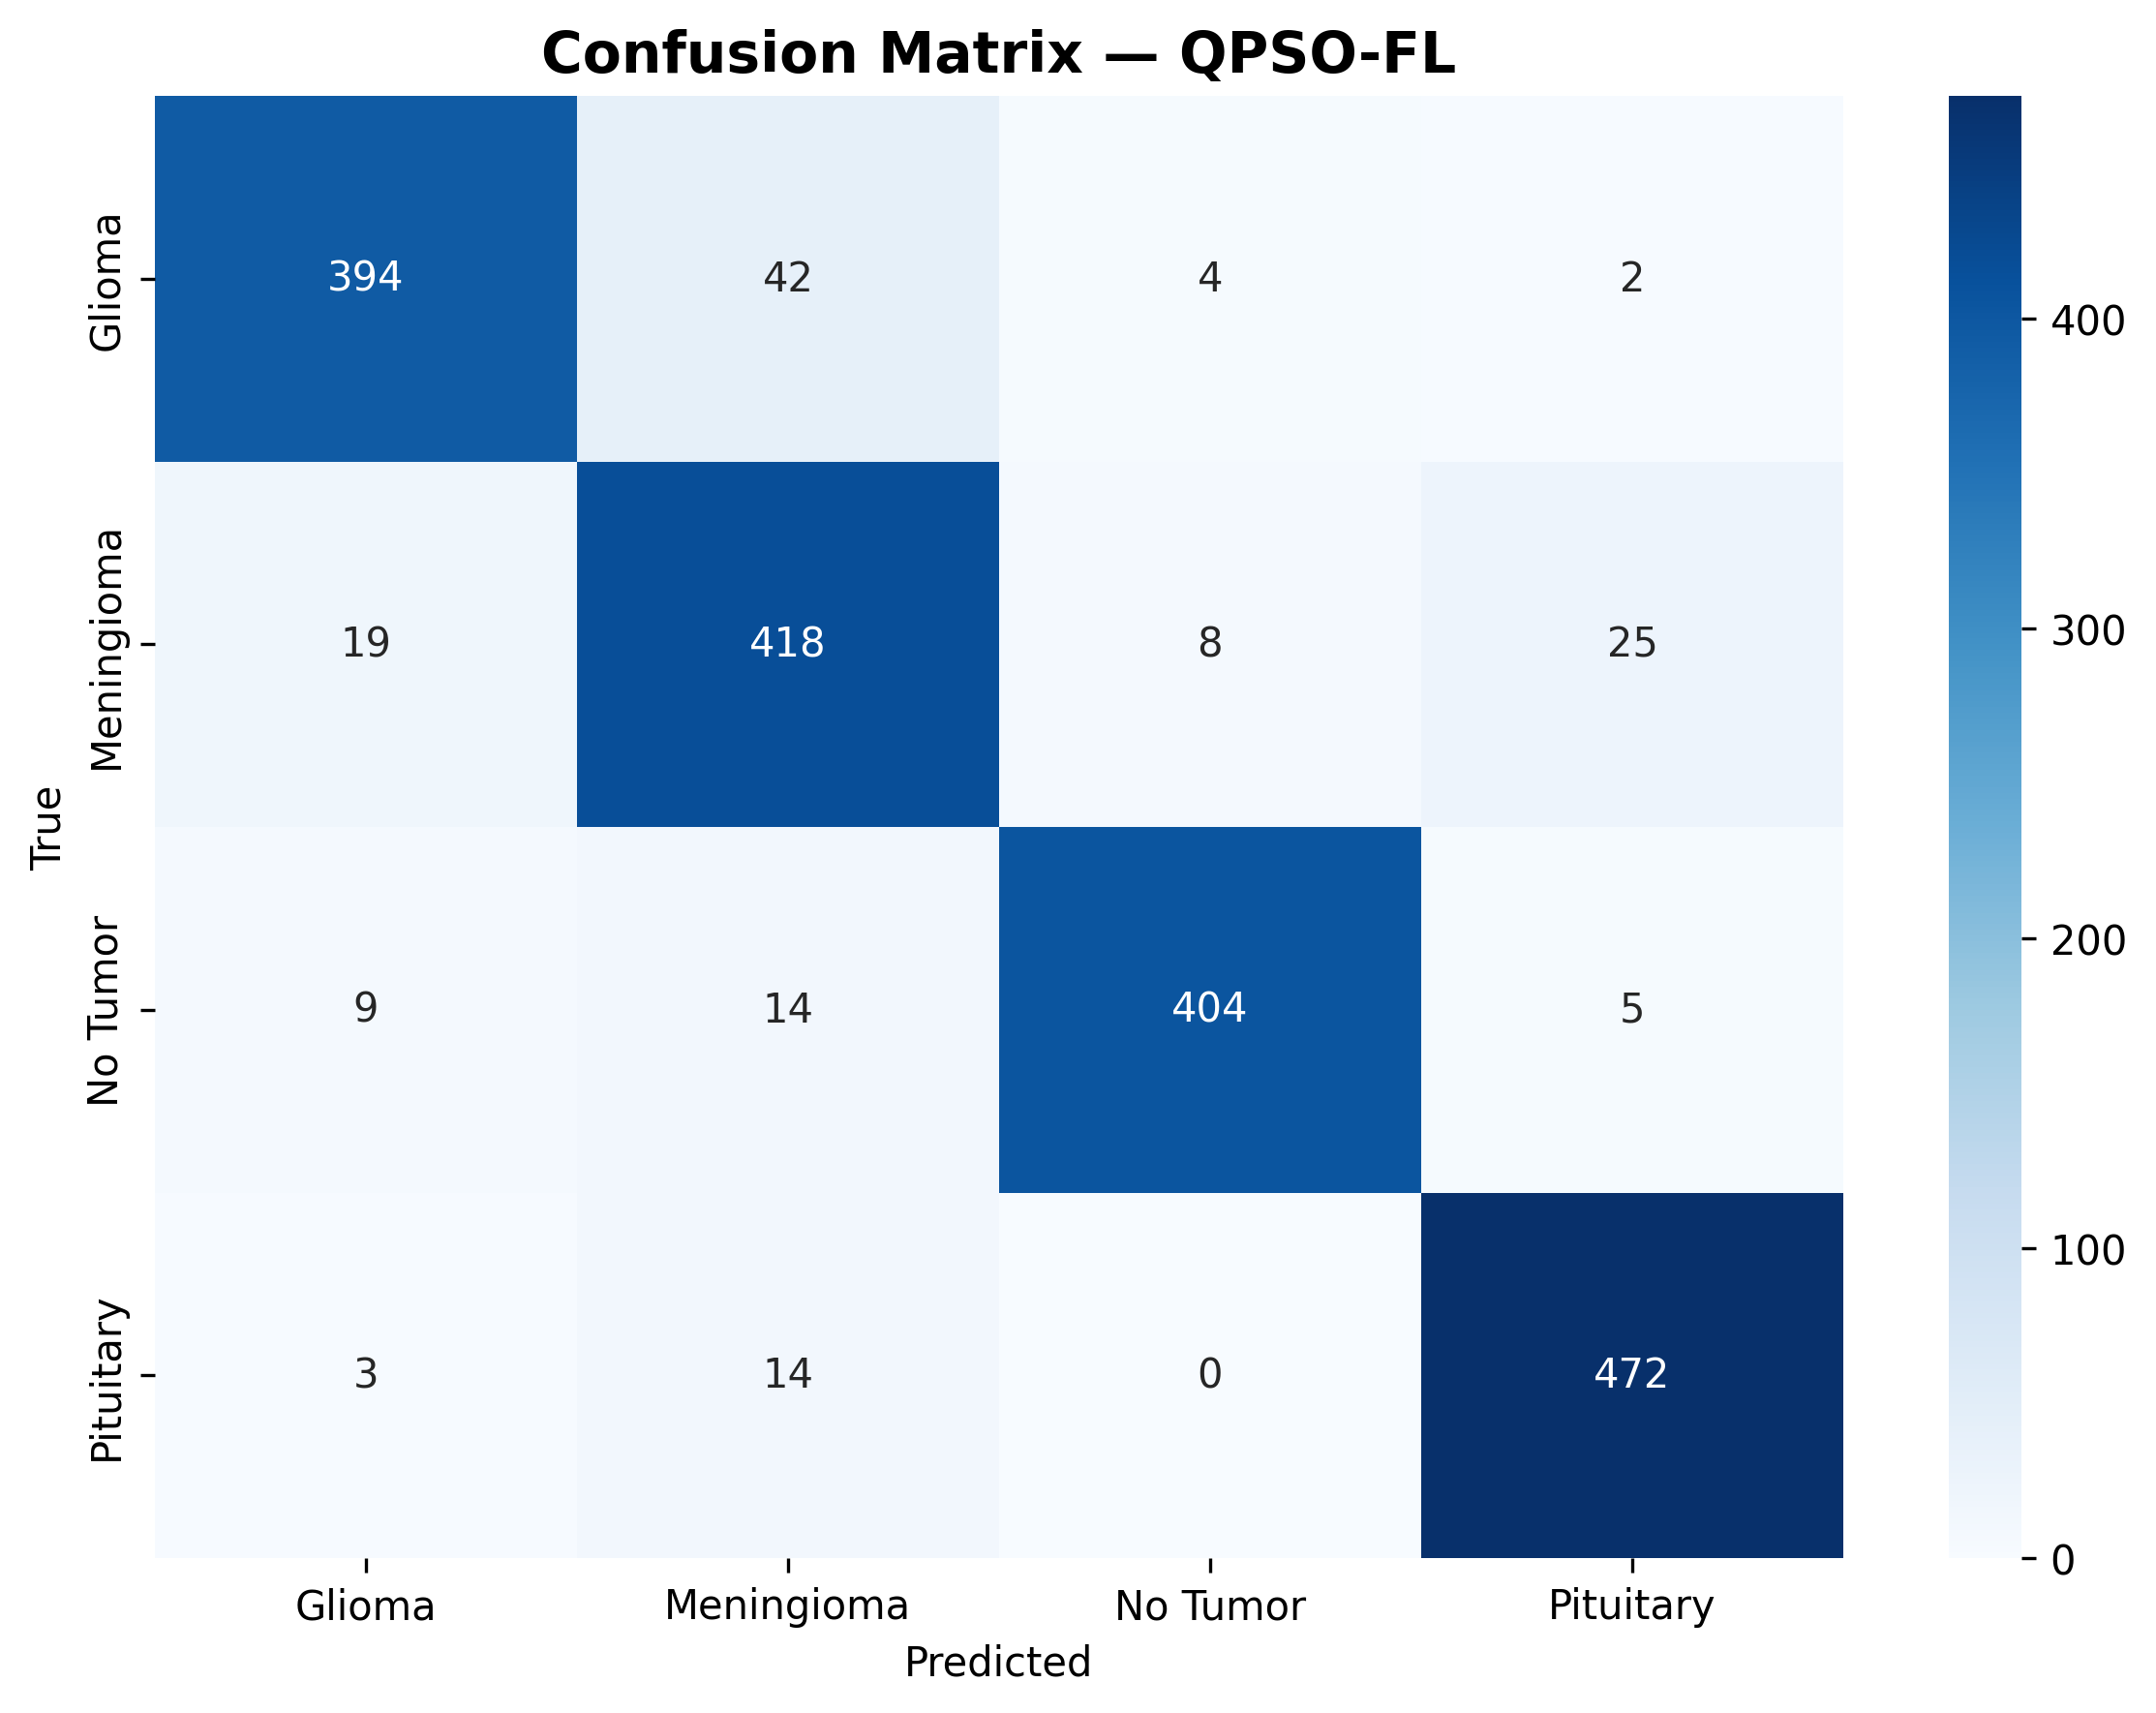
\includegraphics[width=0.48\columnwidth]{s2_cm_qpso.png}}
\caption{Confusion matrices --- Setup 2. Left: FedAvg. Right: FedQPSO. FedAvg shows Meningioma/Glioma confusions from label-skew bias.}
\label{fig:cm_s2}
\end{figure}

\subsection{Stability Analysis}

\begin{table}[t]
\caption{Accuracy Curve Stability}
\label{tab:stability}
\begin{center}
\begin{tabular}{llccc}
\hline
\textbf{Setup} & \textbf{Metric} & \textbf{FedAvg} & \textbf{FedProx} &
\textbf{FedQPSO}\\
\hline
\multirow{2}{*}{S1} & Max round drop (pp) & $-$11.51 & $-$8.46 &
\textbf{$-$2.45}\\
 & Round-to-round std (pp) & $\approx$4.0 & $\approx$4.0 & \textbf{2.22}\\
\hline
\multirow{2}{*}{S2} & Max round drop (pp) & $-$14.78 & $-$9.93 &
\textbf{$-$3.38}\\
 & Round-to-round std (pp) & 4.08 & 4.25 & \textbf{2.16}\\
\hline
\end{tabular}
\end{center}
\end{table}

As shown in Table~\ref{tab:stability}, FedQPSO's round-to-round volatility is
approximately \textbf{half} that of FedAvg and FedProx in both setups. The
largest drop across all 200 FedQPSO rounds (3.38 pp, Setup 2) is smaller than
FedAvg's single largest crash in the \emph{easier} natural heterogeneity
condition (11.51 pp). The fitness evaluation step prevents destabilizing weight
combinations from ever being committed to the global model.

% ============================================================
\section{Discussion}
\label{sec:discussion}
% ============================================================

\subsection{Why FedQPSO Is Fairer}
FedAvg's weighted average systematically over-represents large clients (Client
3 has 3.5$\times$ the data of Client 1, giving proportionally more influence
on every aggregated model). FedProx slows all clients equally but does not
redistribute influence. FedQPSO jointly optimizes each layer against a
\textbf{balanced combined validation set} from all three clients. A weight
configuration that performs well for Clients 2 and 3 but poorly for Client 1
yields high aggregate validation loss and is rejected. The fitness search
therefore naturally converges toward weights that minimize loss
\emph{simultaneously across all clients} --- an implicit fairness constraint
requiring no explicit fairness regularizer.

\subsection{The Role of Algorithm Design: Naive vs.\ Layer-by-Layer QPSO}
Our Phase~3 experiments with a naive whole-model QPSO (blind perturbation of
all 120K parameters simultaneously, no fitness evaluation) produced
catastrophic results: 77.3\% accuracy under label skew versus FedAvg's
90.56\% --- a 13.26 pp deficit. The layer-by-layer redesign with
validation-loss fitness evaluation recovered 14.79 pp and exceeded FedAvg in
both setups. The critical difference: without evaluating the result of
perturbation, QPSO is indistinguishable from deliberate noise injection. With
fitness evaluation, it becomes a genuine optimization procedure.

\subsection{Global Accuracy as a Misleading Metric}
When FedAvg achieved its peak global accuracy of 90.56\% (Setup 2), Client 1
was simultaneously at 52.92\% --- barely above chance. Under FedQPSO, the same
client was at 80.83\% at FedQPSO's own peak of 92.09\%. Global test accuracy
measured on a balanced combined test set \emph{actively hides} severe
per-client disparities. In healthcare, this inequity is not a statistical
artifact --- it represents patients at smaller hospitals receiving substantially
inferior diagnostic support. We recommend that future FL medical imaging work
\emph{always} report per-client performance alongside global metrics.

\subsection{Clinical Interpretation}
FedQPSO is the \textbf{only} tested algorithm that keeps the weakest client
above 80\% accuracy at convergence under label skew. Its superior Glioma
recall (0.8914 vs.\ 0.8620 for FedProx, 0.8371 for FedAvg under Setup 2)
translates to fewer missed glioma diagnoses. The stability advantage (max
crash $\leq$3.38 pp vs.\ $\leq$14.78 pp for FedAvg) is also clinically
meaningful: a sudden 15 pp degradation in model performance during a deployed
FL round would provide dangerously unreliable diagnostic support until the
next stable round.

\subsection{Computational Trade-offs}
FedQPSO's 9.4$\times$ compute overhead relative to FedAvg (approximately 125
minutes vs.\ 13 minutes for 100 rounds on a P100 GPU) is its only
unambiguous disadvantage. Crucially, this overhead is borne \emph{entirely by
the central server} --- participating hospitals experience identical local
training costs. In offline model development contexts, 2 hours of total
training time is entirely practical. For high-frequency real-time retraining
deployments, the overhead may need to be mitigated through reduced QPSO
iterations or selective layer application.

% ============================================================
\section{Limitations and Future Work}
\label{sec:limitations}
% ============================================================

\textbf{Computational cost:} 9.4$\times$ overhead limits retraining frequency.
Future work should explore reducing $T$ or applying FedQPSO selectively to
high-variance layers only.

\textbf{Client scale:} Only 3 clients were evaluated. Fairness claims should
be validated with 5--10 clients simulating more diverse institutional
configurations and data heterogeneity profiles.

\textbf{Architecture:} SimpleCNN was chosen to isolate aggregation as the
performance variable. It would be valuable to evaluate FedQPSO with deeper
(EfficientNet-B0, MobileNetV3) and pretrained architectures, with appropriate
controls for confounding factors.

\textbf{QPSO hyperparameters:} $\beta = 0.6$ and $T = 5$ were adopted from
the MNIST reference \cite{edla2025mnist} without task-specific tuning.
Sensitivity analyses and adaptive scheduling of $\beta$ may improve results.

\textbf{Single seed:} Run-to-run variance across multiple random seeds was not
measured. Future work should report confidence intervals.

\textbf{Privacy guarantees:} Only structural privacy via FL is provided. Adding
formal differential privacy guarantees (e.g.\ Gaussian gradient noise) may
reduce accuracy but would strengthen privacy claims.

% ============================================================
\section{Conclusion}
\label{sec:conclusion}
% ============================================================

We introduced \textbf{FedQPSO}, a novel federated aggregation algorithm
applying layer-by-layer Quantum Particle Swarm Optimization with
validation-loss fitness evaluation to the problem of equitable brain tumor MRI
classification across heterogeneous clinical sites. Through a four-phase
experimental progression on real-world MRI data, we demonstrated that:

\begin{itemize}
    \item FedQPSO reduces the inter-client performance gap by 72--81\% compared
    to FedAvg, and by 45--56\% compared to FedProx.
    \item FedQPSO is the only method maintaining clinically useful accuracy
    ($\geq$80\%) at the weakest client under label skew.
    \item FedQPSO achieves the highest Glioma recall in both experimental
    conditions and demonstrates the most stable accuracy trajectories.
    \item FedQPSO's statistical advantage over FedAvg scales with heterogeneity
    severity (Cohen's $d$: $0.35 \to 1.26$).
    \item The fairness benefit arises from an implicit mechanism: combined
    cross-client validation fitness evaluation, requiring no explicit fairness
    objective.
\end{itemize}

These results establish FedQPSO as the preferred aggregation strategy for
fairness-critical federated deployments in multi-institutional medical imaging
when client equity is a primary objective and the 9$\times$ compute overhead
is acceptable.

% ============================================================
\section*{Acknowledgment}
The authors acknowledge the support of the Department of Computer Science \&
Engineering, Matrusri Engineering College. Compute resources were provided via
Kaggle's GPU platform (Tesla P100-16GB). The Masoud Brain Tumor MRI dataset
and the BRISC 2025 dataset, both publicly available on Kaggle, are gratefully
acknowledged.

% ============================================================
\begin{thebibliography}{00}

\bibitem{mcmahan2017}
H.~B. McMahan, E.~Moore, D.~Ramage, S.~Hampson, and B.~A. y~Arcas,
``Communication-efficient learning of deep networks from decentralized data,''
in \textit{Proc.\ 20th Int.\ Conf.\ Artif.\ Intell.\ Stat.\ (AISTATS)},
Fort Lauderdale, FL, USA, Apr.\ 2017, pp.~1273--1282.

\bibitem{li2020fedprox}
T.~Li, A.~K. Sahu, M.~Zaheer, M.~Sanjabi, A.~Smola, and V.~Smith,
``Federated optimization in heterogeneous networks,''
in \textit{Proc.\ 3rd Conf.\ Mach.\ Learn.\ Syst.\ (MLSys)}, Austin, TX, USA,
Mar.\ 2020, pp.~429--450.

\bibitem{karimireddy2020scaffold}
S.~P. Karimireddy, S.~Kale, M.~Mohri, S.~Reddi, S.~Stich, and A.~T. Suresh,
``SCAFFOLD: Stochastic controlled averaging for federated learning,''
in \textit{Proc.\ 37th Int.\ Conf.\ Mach.\ Learn.\ (ICML)}, Vienna, Austria,
Jul.\ 2020, pp.~5132--5143.

\bibitem{zhao2018}
J.~Zhao, M.~Li, J.~Xu, and W.~Li,
``Federated learning with non-IID data,''
\textit{arXiv:1806.00582}, Jun.\ 2018.

\bibitem{sun2004qpso}
J.~Sun, B.~Feng, and W.~Xu,
``Particle swarm optimization with particles having quantum behavior,''
in \textit{Proc.\ 2004 Congr.\ Evol.\ Comput.\ (CEC)}, Portland, OR, USA,
Jun.\ 2004, vol.~1, pp.~325--331.

\bibitem{sheller2018}
M.~J. Sheller, G.~A. Reina, B.~Edwards, J.~Martin, and S.~Bakas,
``Multi-institutional deep learning modeling without sharing patient data:
A feasibility study on brain tumor segmentation,''
in \textit{Proc.\ Int.\ MICCAI Brainlesion Workshop}, Granada, Spain,
Sep.\ 2018, pp.~92--104.

\bibitem{rieke2020}
N.~Rieke \textit{et al.},
``The future of digital health with federated learning,''
\textit{npj Digit.\ Med.}, vol.~3, no.~1, pp.~1--7, Sep.\ 2020.

\bibitem{sultan2019}
H.~H. Sultan, N.~M. Salem, and W.~Al-Atabany,
``Multi-classification of brain tumor images using deep neural network,''
\textit{IEEE Access}, vol.~7, pp.~69 215--69 225, 2019.

\bibitem{ostrom2021}
Q.~T. Ostrom \textit{et al.},
``CBTRUS statistical report: Primary brain and other central nervous system
tumors diagnosed in the United States in 2014--2018,''
\textit{Neuro-oncology}, vol.~23, no.~suppl\_3, pp.~iii1--iii105, 2021.

\bibitem{hipaa}
U.S.\ Department of Health \& Human Services,
``Health Insurance Portability and Accountability Act (HIPAA) of 1996,''
Public Law 104-191, 1996.

\bibitem{kennedy1995}
J.~Kennedy and R.~Eberhart,
``Particle swarm optimization,''
in \textit{Proc.\ ICNN'95 --- Int.\ Conf.\ Neural Netw.}, Perth, WA, Australia,
Nov.--Dec.\ 1995, vol.~4, pp.~1942--1948.

\bibitem{fedpso2021}
J.~Park, H.~J. Kim, and J.~Moon,
``FedPSO: Federated learning using particle swarm optimization to
reduce communication costs,''
\textit{Sensors}, vol.~21, no.~2, p.~600, Jan.\ 2021.

\bibitem{kulkarni2020pfl}
V.~Kulkarni, M.~Kulkarni, and A.~Pant,
``Survey of personalization techniques for federated learning,''
in \textit{Proc.\ 2020 4th World Conf.\ Smart Trends Syst., Secur. Sustainability},
London, UK, Jul.\ 2020, pp.~794--797.

\bibitem{masoud}
M. Nickparvar,
``Brain tumor MRI dataset,''
Kaggle, 2021. [Online]. Available:
\url{https://www.kaggle.com/datasets/masoudnickparvar/brain-tumor-mri-dataset}

\bibitem{brisc}
BRISC Dataset Contributors,
``BRISC 2025 brain tumor classification dataset,''
Kaggle, 2025. [Online]. Available:
\url{https://www.kaggle.com/datasets/briscdataset/}

\bibitem{edla2025mnist}
Divyansh Teja Edla,
``Enhancing federated learning with quantum-inspired particle swarm
optimization: An {IID} {MNIST} study,'' (Paper ID: CSE-104)
in \textit{Proc.\ AICTE Sponsored Natl.\ Conf.\ Innovations, Challenges
and Solutions in Eng., Sci.\ and Technol.\ (NCICSET'25)},
Sri Indu College of Engineering and Technology, Hyderabad, India,
Dec.\ 17--18, 2025.

\end{thebibliography}

\end{document}

\label{tab:hyperparams}
\begin{center}
\begin{tabular}{lc}
\hline
\textbf{Parameter} & \textbf{Value}\\
\hline
Max communication rounds & 100\\
Local epochs per round & 1\\
Local optimizer & Adam\\
Learning rate & 0.01\\
Batch size & 64\\
Image size & $112 \times 112$\\
FedProx $\mu$ & 0.01\\
FedQPSO $\beta$ & 0.6 (static)\\
FedQPSO QPSO iterations per layer $T$ & 5\\
Early stopping patience & 15 rounds\\
Hardware & Tesla P100-16GB (Kaggle)\\
Framework & PyTorch 2.x, Python 3.12\\
Random seed & 42\\
\hline
\end{tabular}
\end{center}
\end{table}

\subsection{Evaluation Metrics}
Primary: global test accuracy, per-class precision / recall / F1, ROC-AUC
(per-class and micro-average). Fairness: per-client validation accuracy
standard deviation ($\sigma$) and max-minus-min gap across clients. Stability:
maximum single-round accuracy drop and round-to-round volatility (standard
deviation of accuracy deltas). Statistical significance: paired two-tailed
$t$-test on per-round accuracy sequences, Cohen's $d$ as effect size.
Convergence speed: rounds to first reach 80\% global accuracy.

% ============================================================
\section{Results}
\label{sec:results}
% ============================================================

\subsection{Global Accuracy}

Table~\ref{tab:global_s1} summarizes global test accuracy for Setup 1, and
Table~\ref{tab:global_s2} for Setup 2.

\begin{table}[t]
\caption{Global Test Accuracy --- Setup 1 (Natural Heterogeneity)}
\label{tab:global_s1}
\begin{center}
\begin{tabular}{lcc}
\hline
\textbf{Metric} & \textbf{FedAvg} & \textbf{FedQPSO}\\
\hline
Best Accuracy (\%) & \textbf{95.80} (r83) & 95.14 (r89)\\
Final Accuracy (\%) & 93.29 (r98) & \textbf{93.78} (r100)\\
Rounds run & 98$^\dagger$ & 100\\
Rounds to 80\% & 11 & \textbf{9}\\
Avg.\ round time (s) & 7.84 & 75.09\\
\multicolumn{4}{l}{{\small $^\dagger$Early stopping: $\geq$95\% accuracy reached, patience = 15 rounds.}}
\end{tabular}
\end{center}
\end{table}

\begin{table}[t]
\caption{Global Test Accuracy --- Setup 2 (Moderate Label Skew)}
\label{tab:global_s2}
\begin{center}
\begin{tabular}{lcc}
\hline
\textbf{Metric} & \textbf{FedAvg} & \textbf{FedQPSO}\\
\hline
Best Accuracy (\%) & 90.56 (r94) & \textbf{92.09} (r98)\\
Final Accuracy (\%) & 88.16 (r100) & \textbf{91.43} (r100)\\
Rounds to 80\% & 35 & \textbf{19}\\
Avg.\ round time (s) & 8.03 & 74.92\\
\hline
\end{tabular}
\end{center}
\end{table}

Accuracy curves for both setups are shown in Fig.~\ref{fig:curves_s1} and
Fig.~\ref{fig:curves_s2}. FedQPSO's accuracy trajectory is visibly smoother
than both baselines, with substantially lower oscillation.

\begin{figure}[t]
\centerline{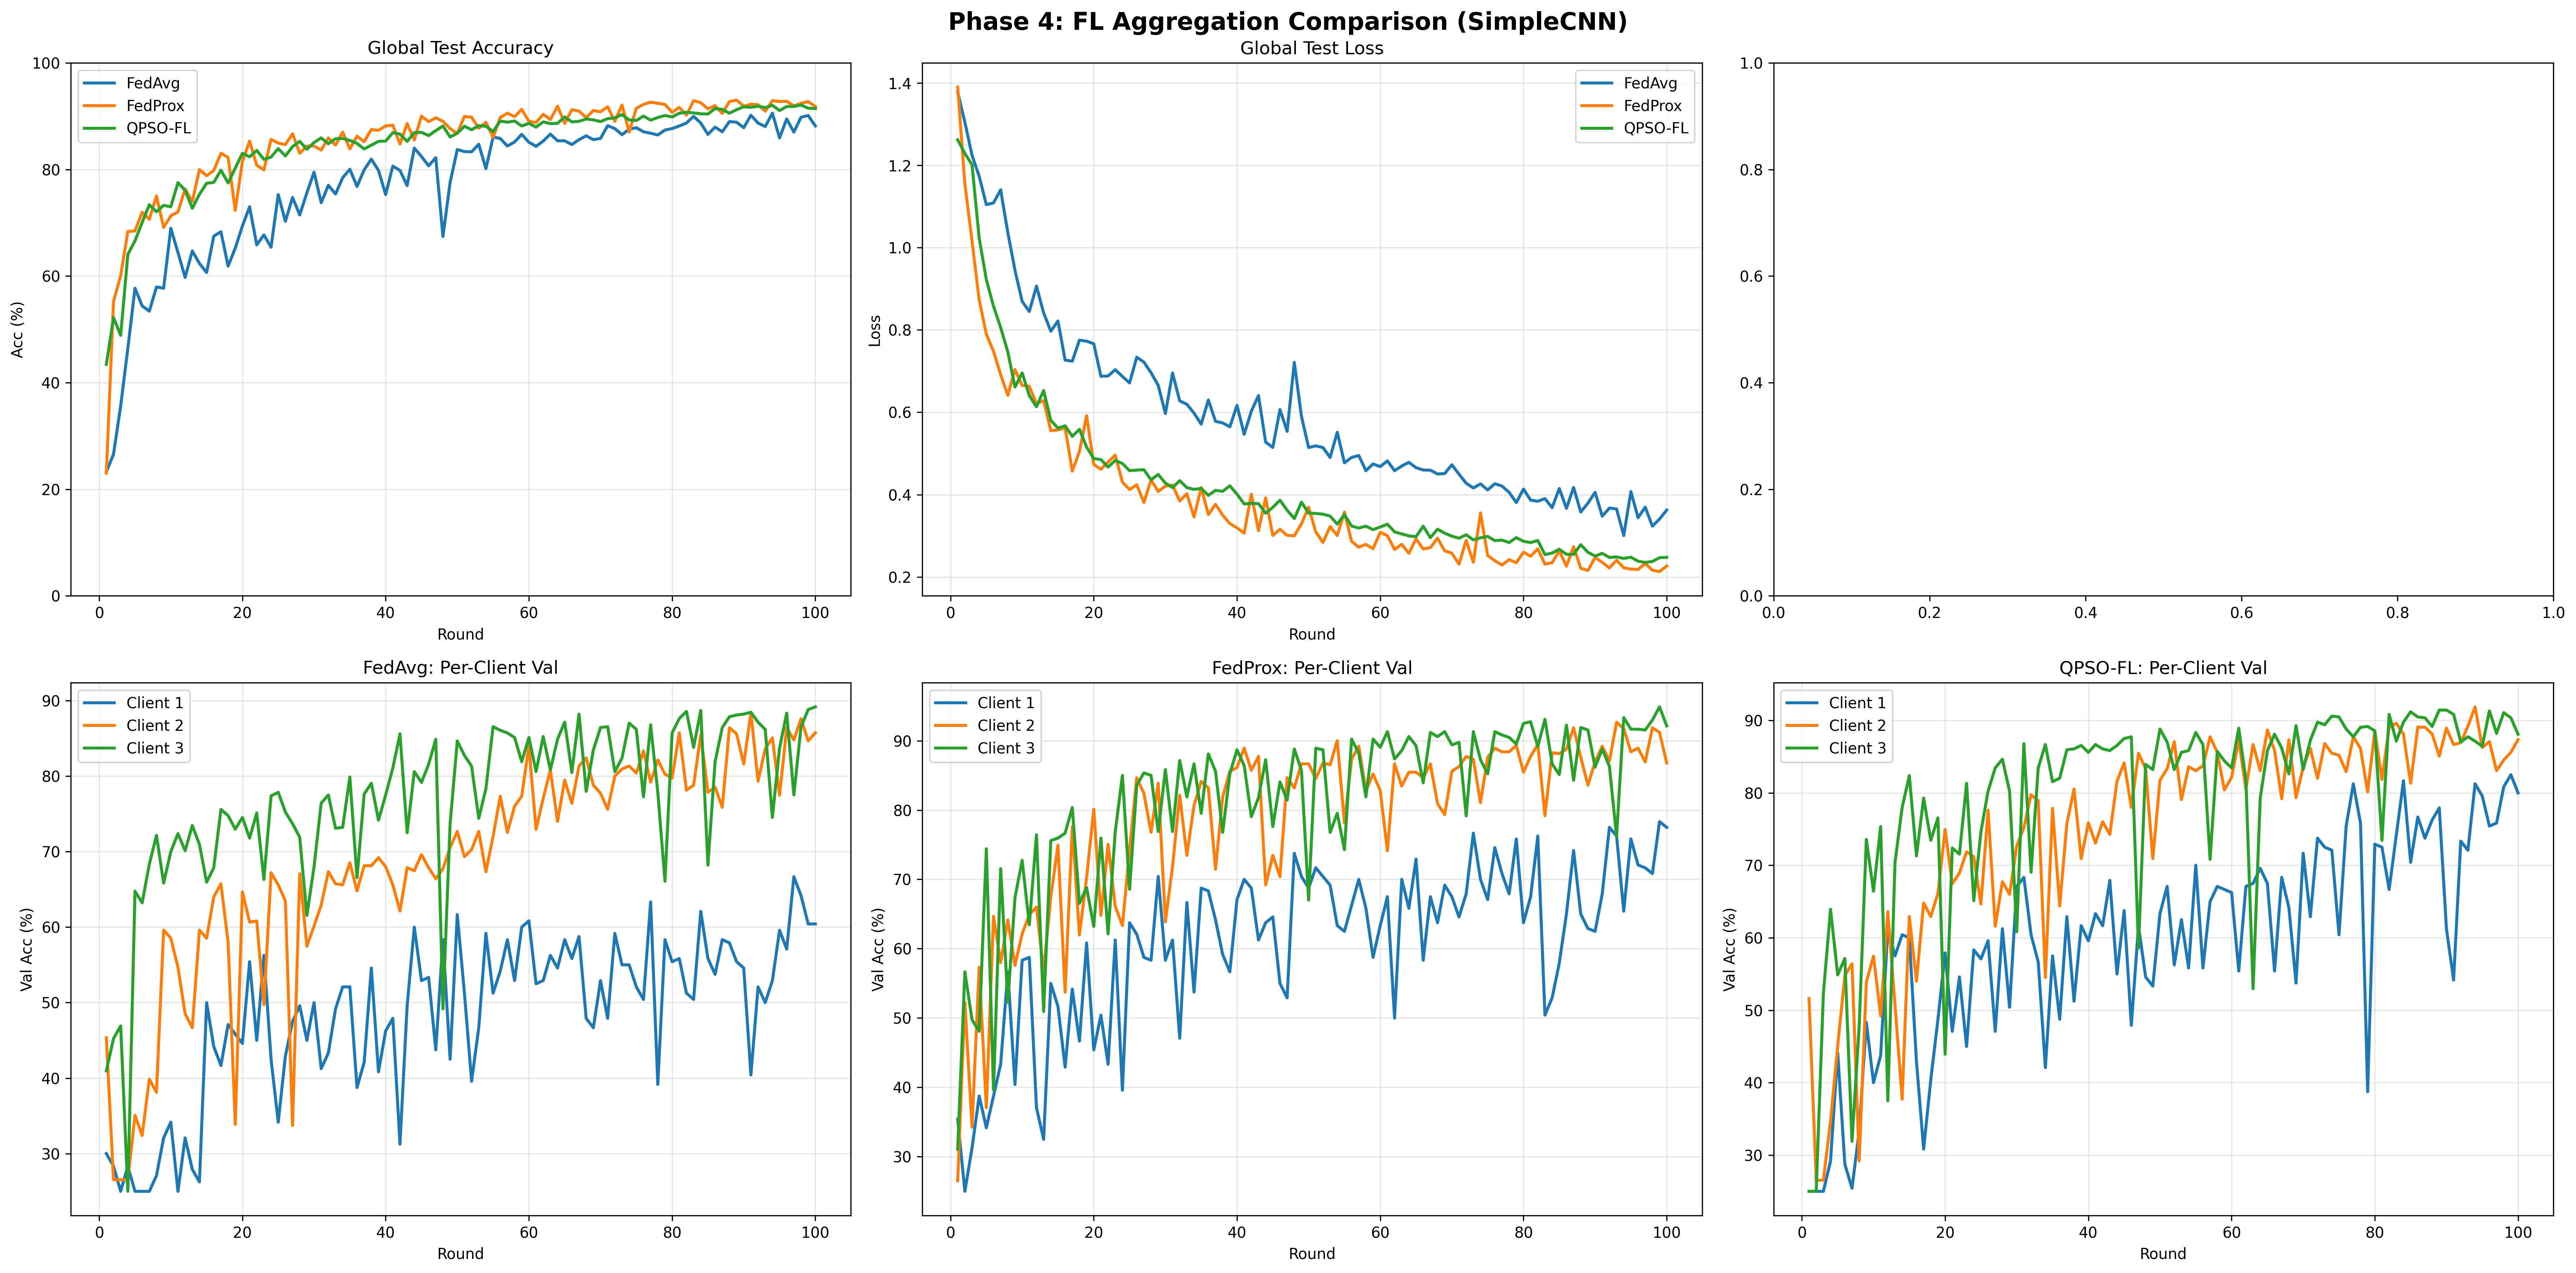
\includegraphics[width=\columnwidth]{s1_comparison.png}}
\caption{Accuracy and loss curves over 100 rounds --- Setup 1 (Natural
Heterogeneity). FedQPSO exhibits markedly lower round-to-round
volatility than FedAvg.}
\label{fig:curves_s1}
\end{figure}

\begin{figure}[t]
\centerline{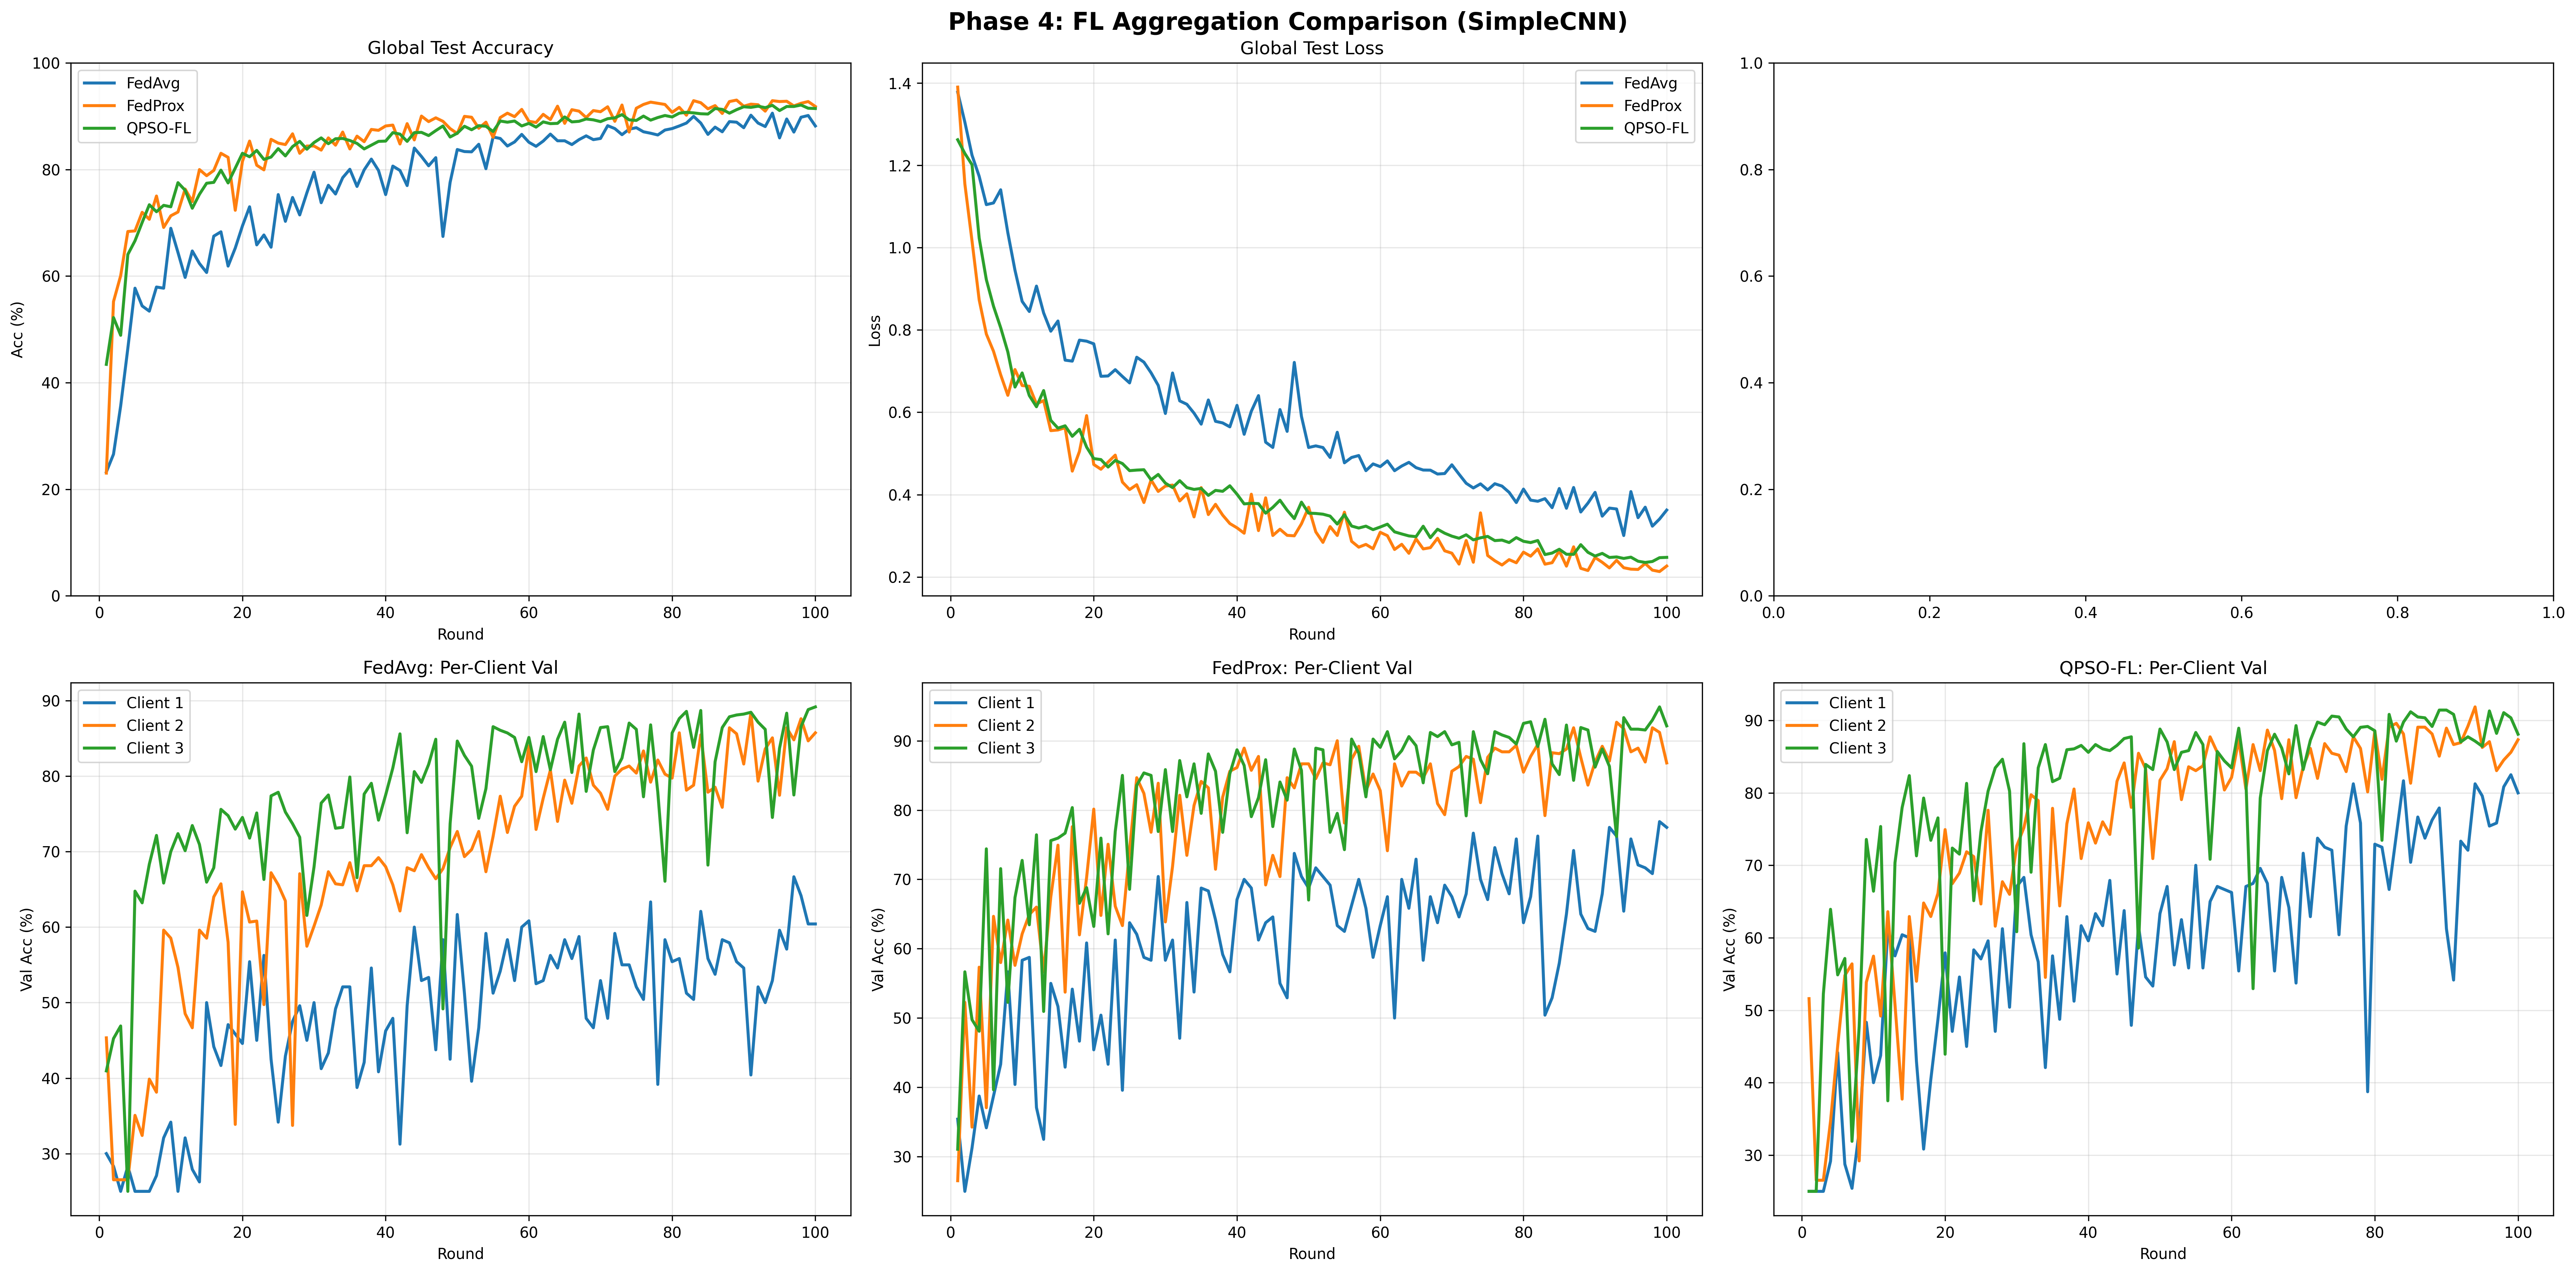
\includegraphics[width=\columnwidth]{s2_comparison.png}}
\caption{Accuracy and loss curves over 100 rounds --- Setup 2 (Moderate Label
Skew). FedAvg degrades significantly faster; FedQPSO shows superior fairness.}
\label{fig:curves_s2}
\end{figure}

\subsection{Per-Class Classification Performance}

Table~\ref{tab:perclass} reports the F1-score and recall for each tumor class
at the respective best-round model checkpoint for each method.

\begin{table}[t]
\caption{Per-Class F1-Score and Recall at Best Model Checkpoint
(S1 = Setup 1, S2 = Setup 2)}
\label{tab:perclass}
\begin{center}
\renewcommand{\arraystretch}{1.15}
\begin{tabular}{llccc}
\hline
\textbf{Setup} & \textbf{Class} & \textbf{FedAvg} & \textbf{FedProx} &
\textbf{FedQPSO}\\
\hline
\multirow{5}{*}{S1 F1}
 & Glioma    & 0.9438 & 0.9420 & \textbf{0.9560}\\
 & Meningioma & 0.9378 & \textbf{0.9394} & 0.9211\\
 & No Tumor  & 0.9663 & \textbf{0.9790} & 0.9602\\
 & Pituitary & 0.9828 & \textbf{0.9846} & 0.9686\\
 & Macro Avg & 0.9577 & \textbf{0.9612} & 0.9515\\
\hline
\multirow{5}{*}{S2 F1}
 & Glioma    & 0.8841 & 0.9039 & \textbf{0.9089}\\
 & Meningioma & 0.8458 & \textbf{0.8921} & 0.8727\\
 & No Tumor  & 0.9447 & \textbf{0.9554} & 0.9528\\
 & Pituitary & 0.9491 & \textbf{0.9689} & 0.9507\\
 & Macro Avg & 0.9059 & \textbf{0.9301} & 0.9213\\
\hline
\multirow{2}{*}{Recall}
 & Glioma (S1) & 0.9118 & 0.9186 & \textbf{0.9593}\\
 & Glioma (S2) & 0.8371 & 0.8620 & \textbf{0.8914}\\
\hline
\end{tabular}
\end{center}
\end{table}

FedQPSO achieves the \textbf{highest Glioma F1 and recall in both setups} --- the
most clinically critical tumor class, where missed diagnoses carry potentially
fatal consequences. Compared to FedAvg under label skew, FedQPSO's Glioma
recall improvement of 5.43 pp corresponds to approximately 24 additional
correctly identified glioma cases per 1,000 patients.

\subsection{Client Fairness --- Primary Finding}

Table~\ref{tab:fairness} presents client fairness metrics. Fig.~\ref{fig:fairness_s1}
and Fig.~\ref{fig:fairness_s2} visualize per-client accuracy distributions.

\begin{table}[t]
\caption{Client Fairness Metrics (Final Round and At-Peak-Round)}
\label{tab:fairness}
\begin{center}
\renewcommand{\arraystretch}{1.15}
\begin{tabular}{llccc}
\hline
\textbf{Setup} & \textbf{Metric} & \textbf{FedAvg} & \textbf{FedProx} &
\textbf{FedQPSO}\\
\hline
\multirow{4}{*}{S1}
 & Cl.\ 1 final (\%) & 83.75 & 91.25 & \textbf{92.08}\\
 & Client $\sigma$ final & 5.28\% & 2.27\% & \textbf{1.56\%}\\
 & Max$-$Min gap (pp) & 12.20 & 5.30 & \textbf{2.32}\\
 & Client $\sigma$ at peak & 9.50\% & 2.79\% & \textbf{1.62\%}\\
\hline
\multirow{4}{*}{S2}
 & Cl.\ 1 final (\%) & 60.42 & 77.50 & \textbf{80.00}\\
 & Client $\sigma$ final & 12.82\% & 6.05\% & \textbf{3.65\%}\\
 & Max$-$Min gap (pp) & 28.75 & 14.64 & \textbf{8.10}\\
 & Client $\sigma$ at peak & 13.38\% & 12.07\% & \textbf{4.23\%}\\
\hline
\end{tabular}
\end{center}
\end{table}

\begin{figure}[t]
\centerline{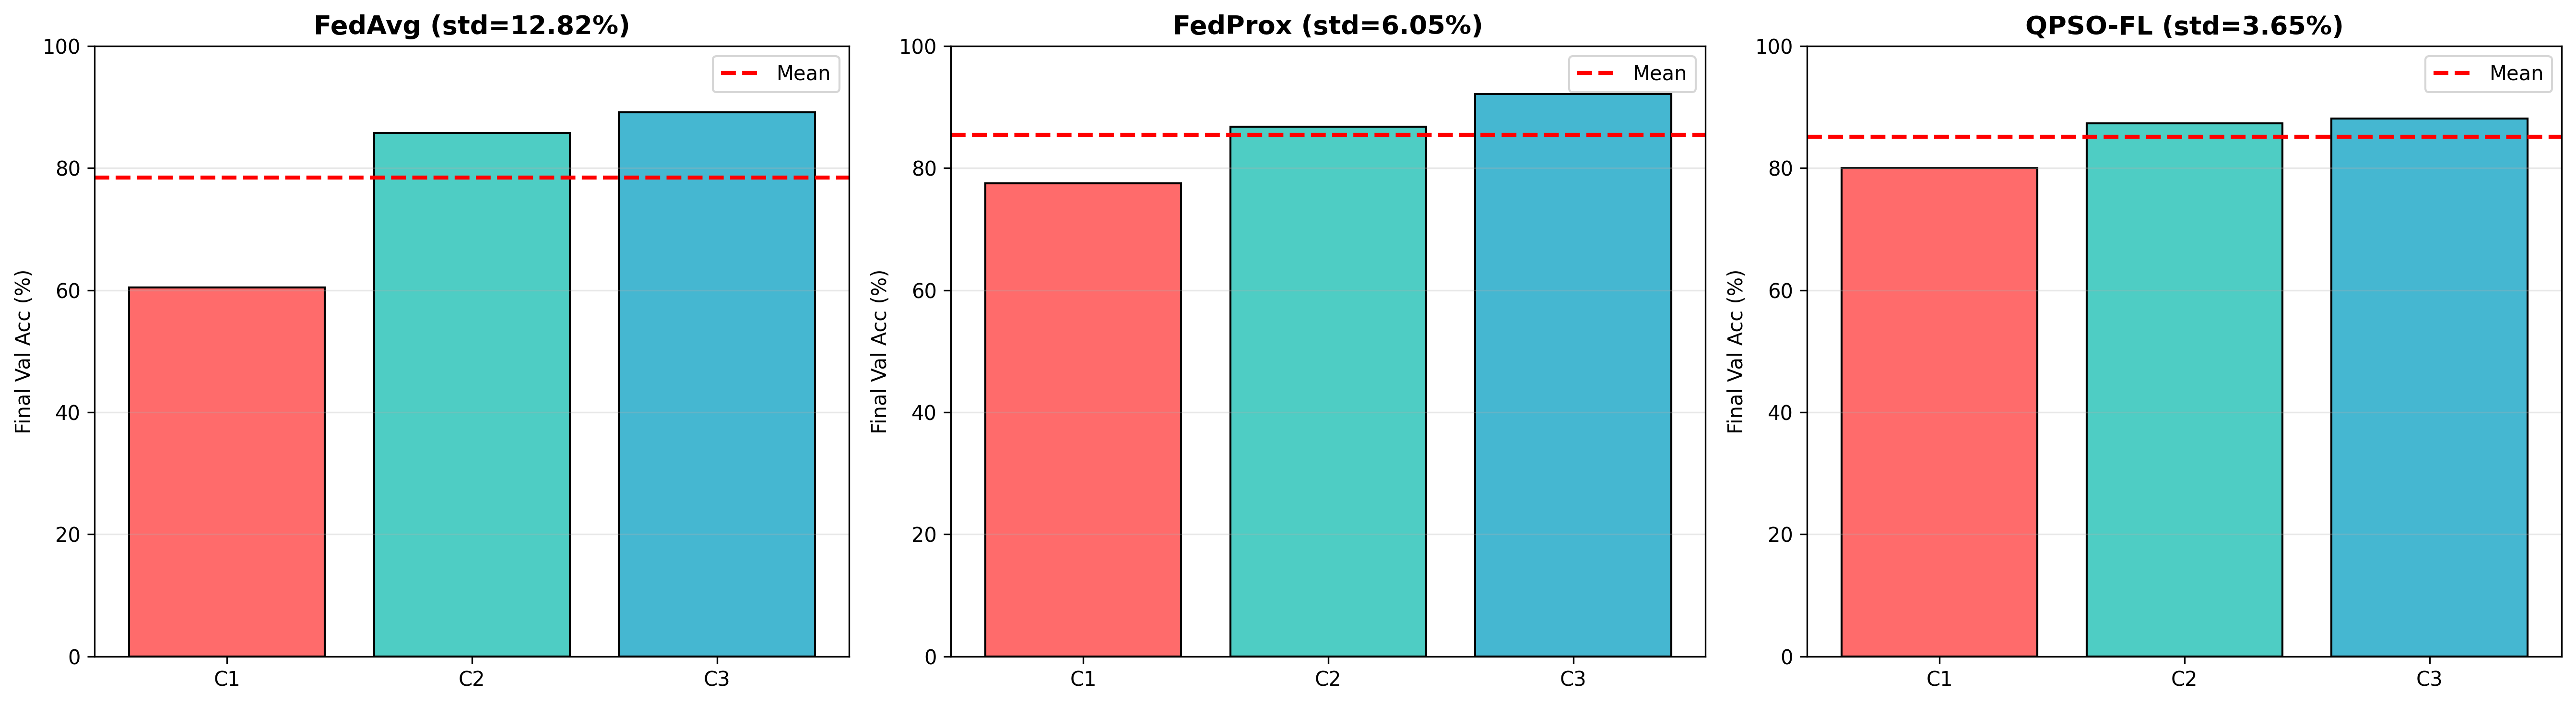
\includegraphics[width=\columnwidth]{s1_fairness.png}}
\caption{Per-client validation accuracy --- Setup 1. When FedAvg peaks
globally at 95.80\%, Client 1 is simultaneously at 75.00\% --- a 20 pp
inequity hidden by the global metric. FedQPSO keeps all clients within 3.5 pp.}
\label{fig:fairness_s1}
\end{figure}

\begin{figure}[t]
\centerline{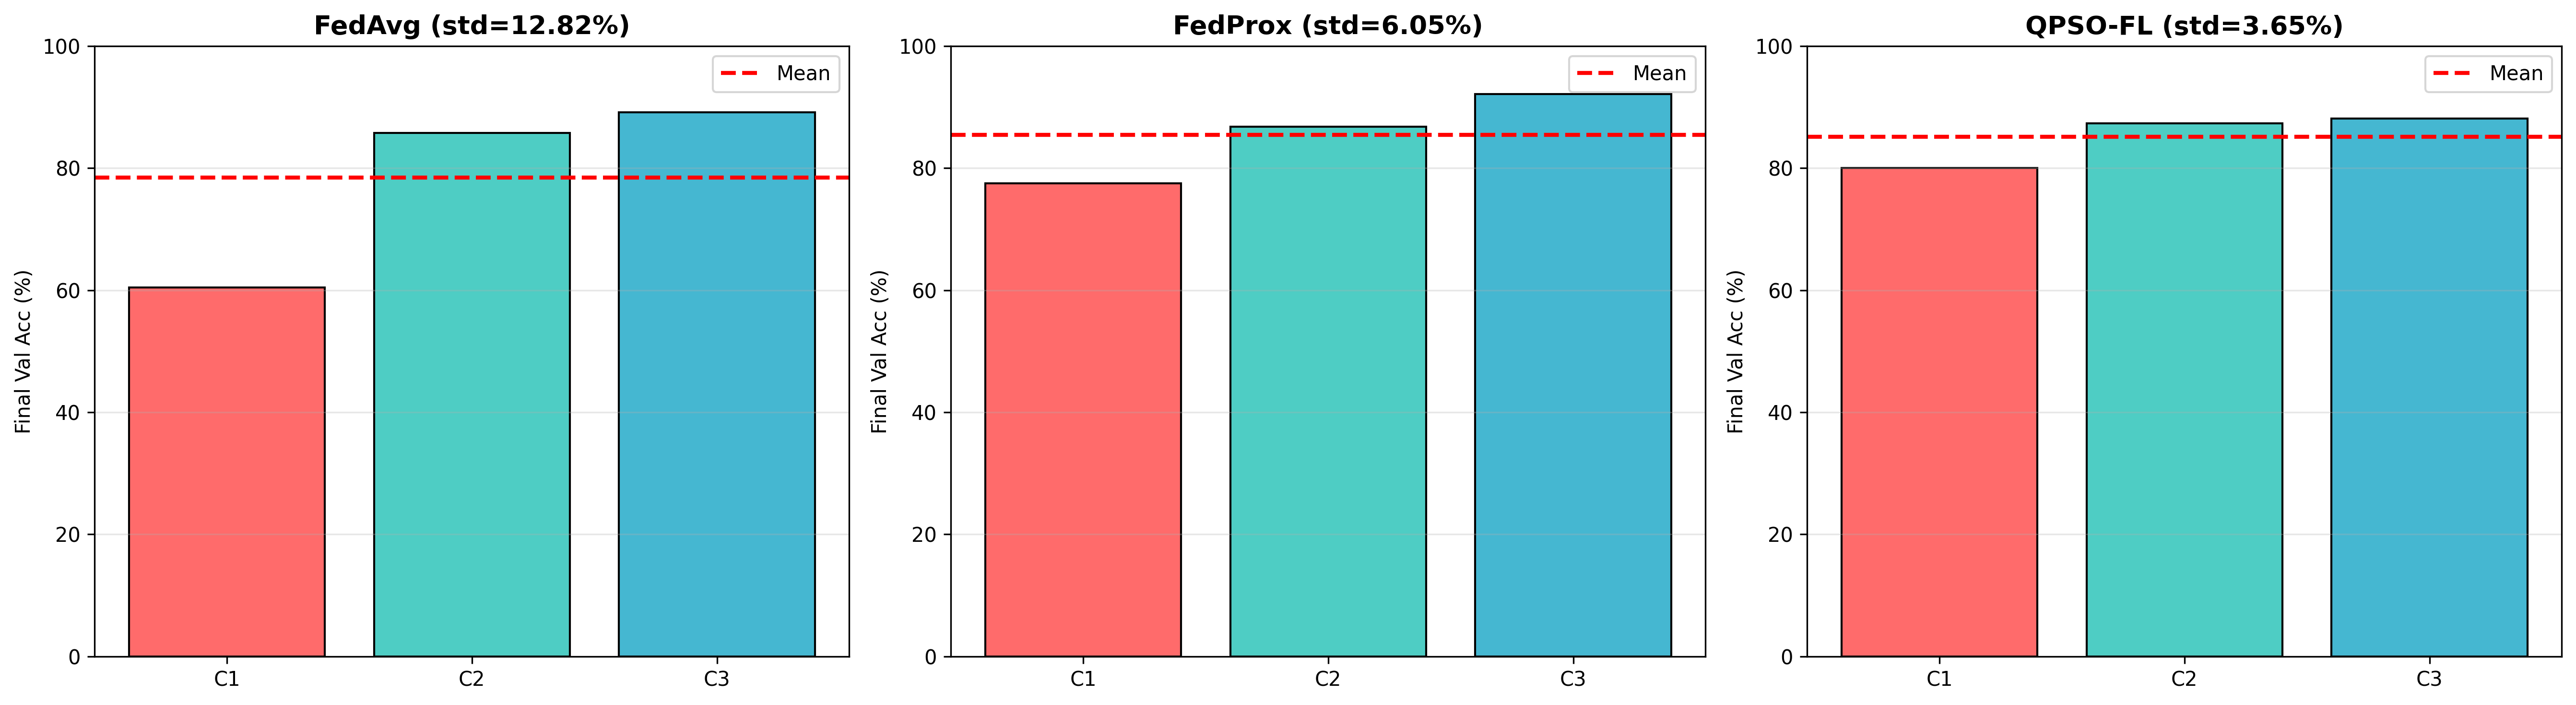
\includegraphics[width=\columnwidth]{s2_fairness.png}}
\caption{Per-client validation accuracy --- Setup 2 (label skew). Under
FedAvg, Client 1 never exceeds 70\% in any of 100 rounds. FedQPSO is
the only method keeping Client 1 above 80\% at convergence.}
\label{fig:fairness_s2}
\end{figure}

The most clinically significant result: at FedAvg's peak global accuracy of
90.56\% (Setup 2), Client~1's validation accuracy was simultaneously
\textbf{52.92\%} --- barely above random chance for a 4-class problem. At
FedQPSO's peak (92.09\%), Client~1 was at \textbf{80.83\%} --- a 27.91 pp
improvement for the weakest hospital at the same moment of best global
performance.

FedQPSO reduces FedAvg's max-min client accuracy gap by \textbf{81\%} in
Setup 1 (12.20 $\to$ 2.32 pp) and \textbf{72\%} in Setup 2 (28.75 $\to$
8.10 pp), and exceeds FedProx by 45--56\% on the same metric. Critically, the
QPSO--FedProx fairness gap \emph{widens} from 0.71 pp to 2.40 pp in client
$\sigma$ as heterogeneity increases --- the mechanism becomes more effective
under harder conditions.

\subsection{Statistical Significance}

Results of paired two-tailed $t$-tests on per-round global accuracy sequences
are summarized in Table~\ref{tab:stats}.

\begin{table}[t]
\caption{Statistical Significance: Paired $t$-Test on Per-Round Accuracy}
\label{tab:stats}
\begin{center}
\begin{tabular}{llcccl}
\hline
\textbf{Setup} & \textbf{Comparison} & $t$ & $p$ & $d$ & \textbf{Sig.}\\
\hline
S1 & FedAvg vs FedQPSO  & 3.43 & 0.000882 & 0.35 & \checkmark \\
S1 & FedAvg vs FedProx  & 1.72 & 0.0879   & 0.17 & $\times$ \\
S2 & FedAvg vs FedQPSO  & 12.59 & $2.91\!\times\!10^{-22}$ & 1.26 & \checkmark \\
S2 & FedAvg vs FedProx  & 13.39 & $5.86\!\times\!10^{-24}$ & 1.34 & \checkmark \\
\hline
\multicolumn{6}{l}{\small \checkmark: $p < 0.05$; \quad $d$: Cohen's $d$ effect size.}
\end{tabular}
\end{center}
\end{table}

Under natural heterogeneity, \textbf{FedQPSO is the only method that
statistically significantly outperforms FedAvg} ($p = 0.000882$). FedProx
fails to reach significance ($p = 0.088$) --- its proximal term is
insufficient when data distributions are only mildly heterogeneous. Under
label skew, both FedQPSO and FedProx achieve overwhelming statistical
separation from FedAvg (Cohen's $d > 1.2$ for both, representing a large
effect). The jump in Cohen's $d$ from 0.35 (Setup 1) to 1.26 (Setup 2)
confirms that FedQPSO's advantage scales with heterogeneity severity.

\subsection{ROC-AUC Analysis}

\begin{table}[t]
\caption{ROC-AUC Per Class and Micro Average}
\label{tab:auc}
\begin{center}
\begin{tabular}{lcccc}
\hline
& \multicolumn{3}{c}{\textbf{Setup 1}} &
  \multicolumn{3}{c}{\textbf{Setup 2}}\\
\cmidrule(lr){2-4}\cmidrule(lr){5-7}
\textbf{Class} & FA & FP & \textbf{FQ} & FA & FP & \textbf{FQ}\\
\hline
Glioma      & 0.988 & 0.988 & \textbf{0.991} & 0.977 & 0.983 & \textbf{0.985}\\
Meningioma  & 0.992 & \textbf{0.993} & 0.986 & 0.970 & \textbf{0.981} & 0.978\\
No Tumor    & 0.998 & \textbf{0.999} & 0.995 & 0.996 & \textbf{0.997} & \textbf{0.997}\\
Pituitary   & \textbf{0.999} & \textbf{0.999} & 0.998 & 0.996 & \textbf{0.997} & \textbf{0.997}\\
Micro Avg   & 0.995 & \textbf{0.996} & 0.993 & 0.986 & \textbf{0.991} & 0.990\\
\hline
\multicolumn{7}{l}{\small FA=FedAvg, FP=FedProx, FQ=FedQPSO.}
\end{tabular}
\end{center}
\end{table}

All three methods achieve clinically excellent AUC (Table~\ref{tab:auc})
across all classes in both setups --- no AUC falls below 0.970. FedQPSO wins
Glioma AUC in \emph{both} setups (0.991 and 0.985). ROC-AUC curves are shown
in Figs.~\ref{fig:roc_s1} and~\ref{fig:roc_s2}.

\begin{figure}[t]
\centerline{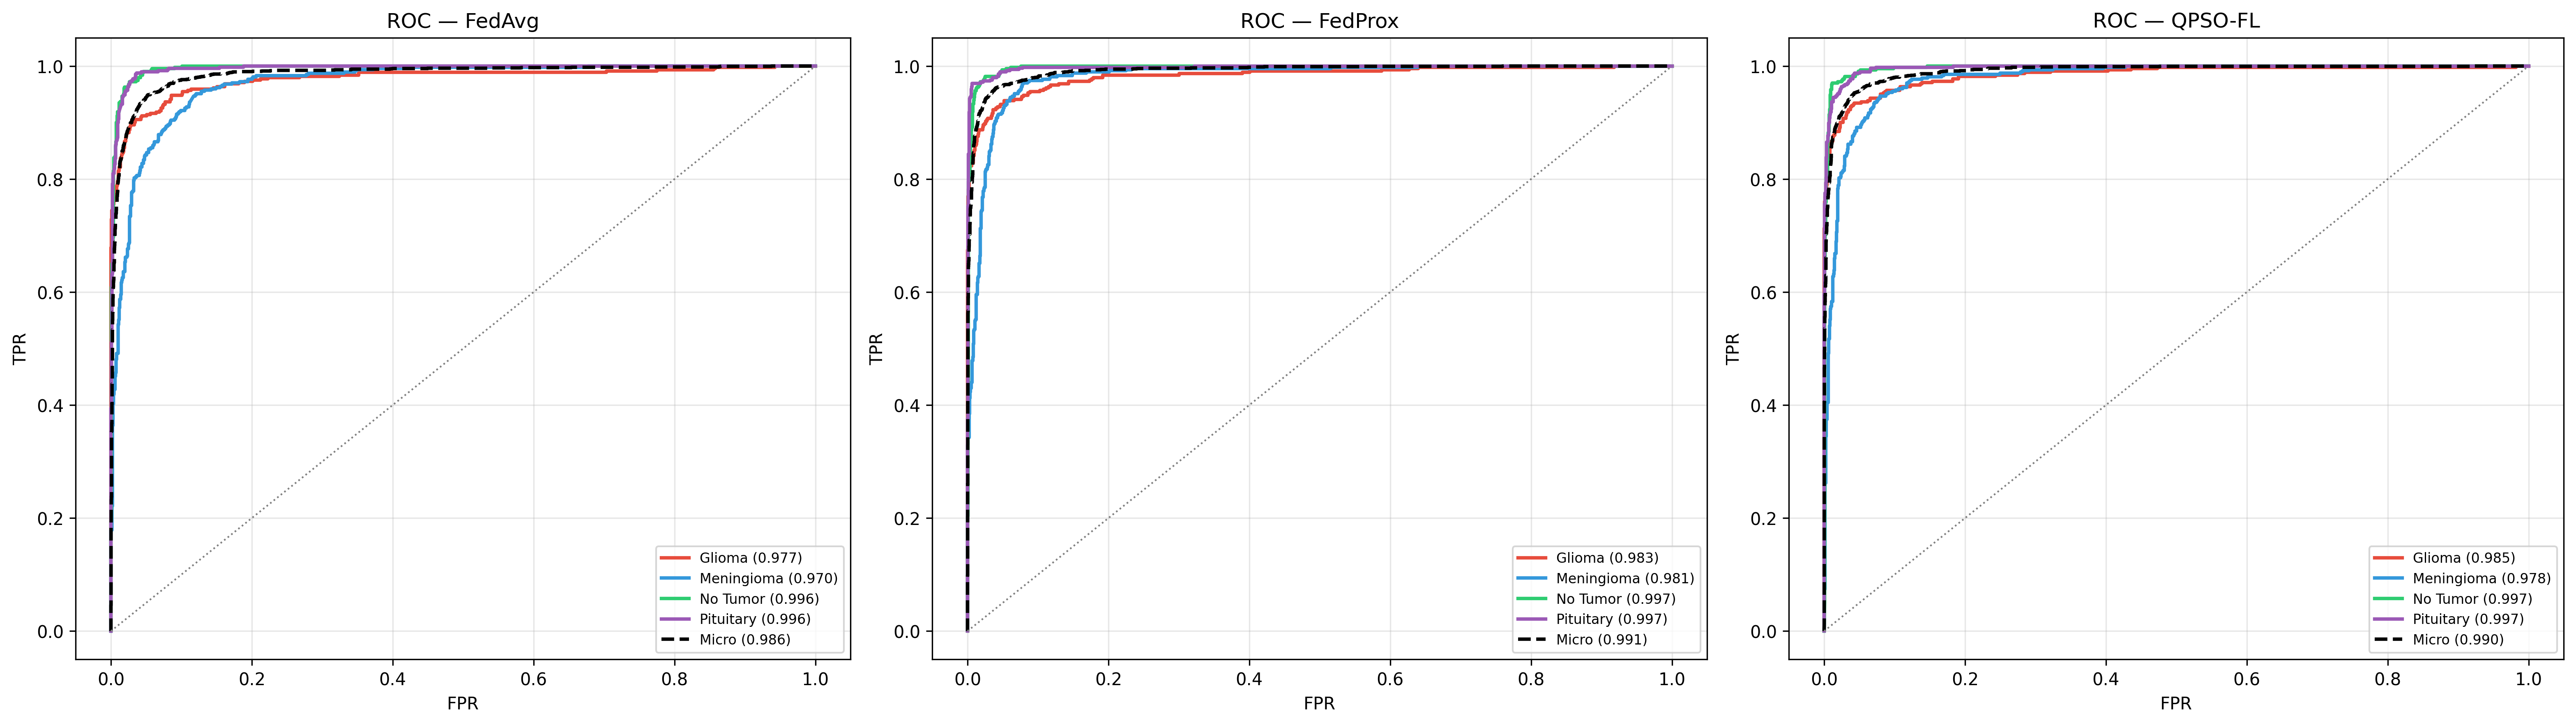
\includegraphics[width=\columnwidth]{s1_roc_auc.png}}
\caption{ROC-AUC curves --- Setup 1. All methods achieve AUC $>$ 0.986 for
every class. FedQPSO leads on the Glioma curve (AUC = 0.991).}
\label{fig:roc_s1}
\end{figure}

\begin{figure}[t]
\centerline{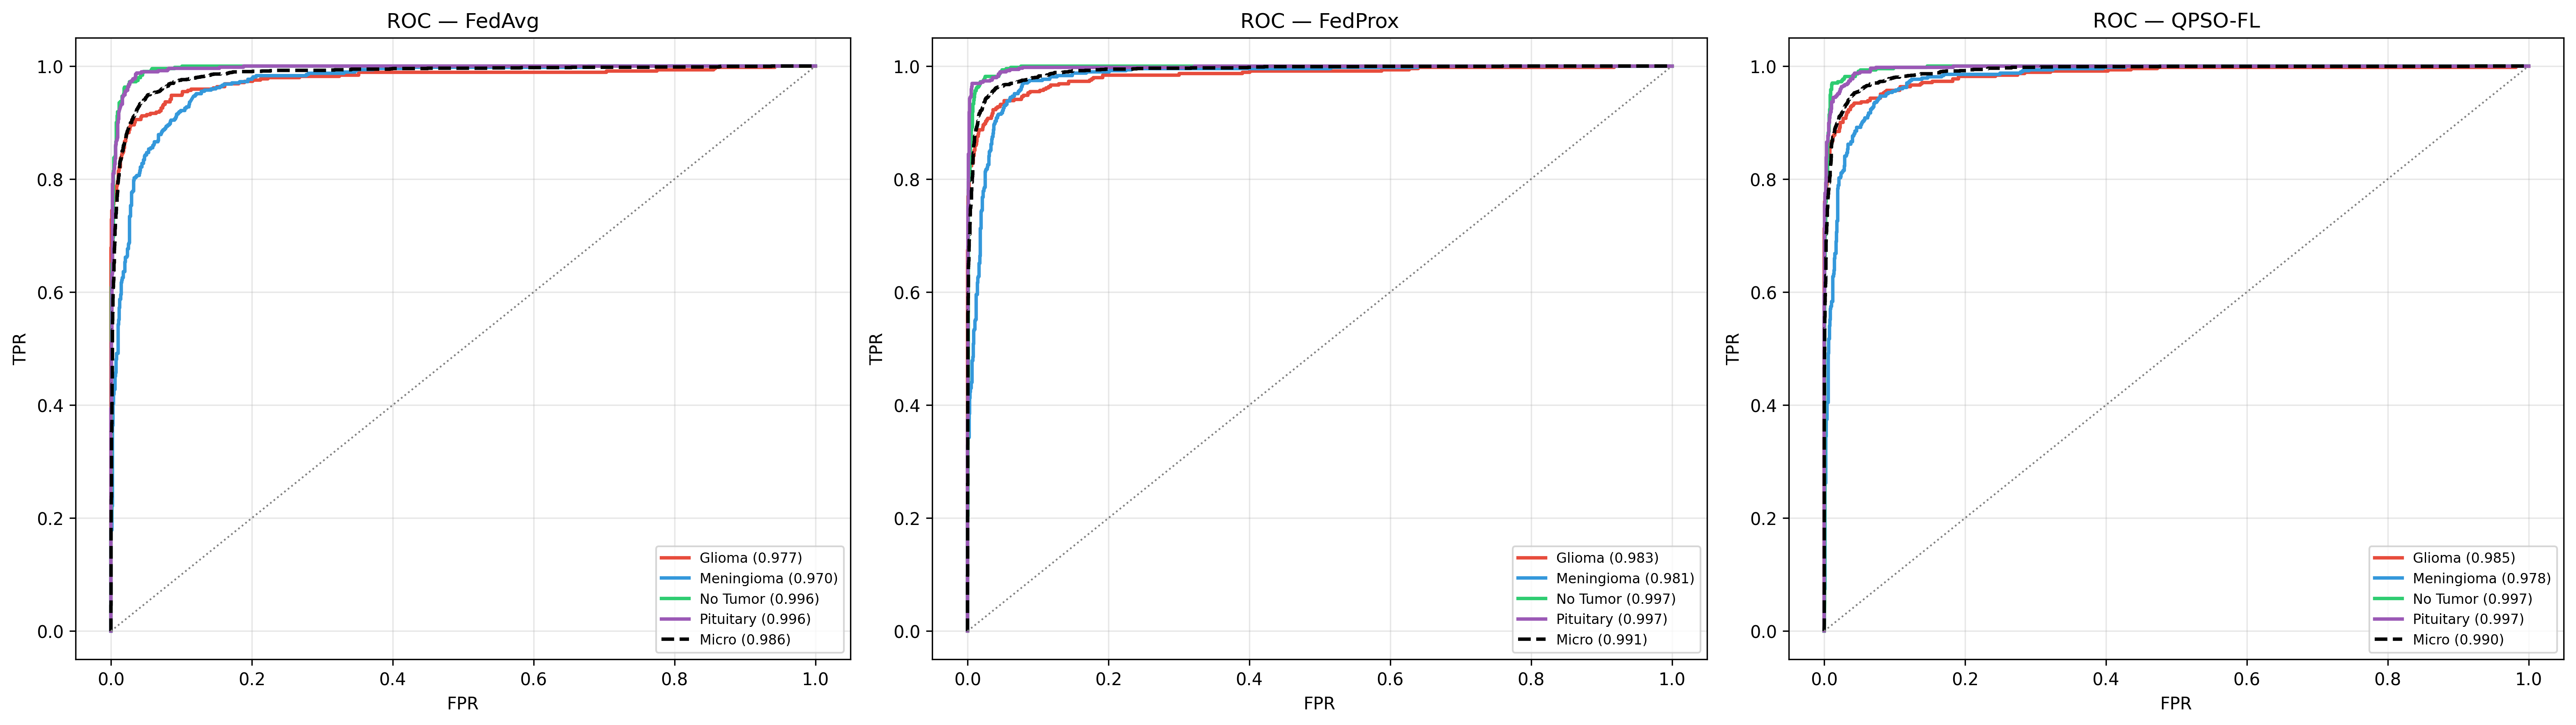
\includegraphics[width=\columnwidth]{s2_roc_auc.png}}
\caption{ROC-AUC curves --- Setup 2. FedAvg Meningioma AUC drops to 0.970
under label skew; FedQPSO maintains above 0.978.}
\label{fig:roc_s2}
\end{figure}

\subsection{Confusion Matrices}

Figs.~\ref{fig:cm_s1} and~\ref{fig:cm_s2} show the confusion matrices for
all three methods at their best-round checkpoints.

\begin{figure}[t]
\centerline{%
  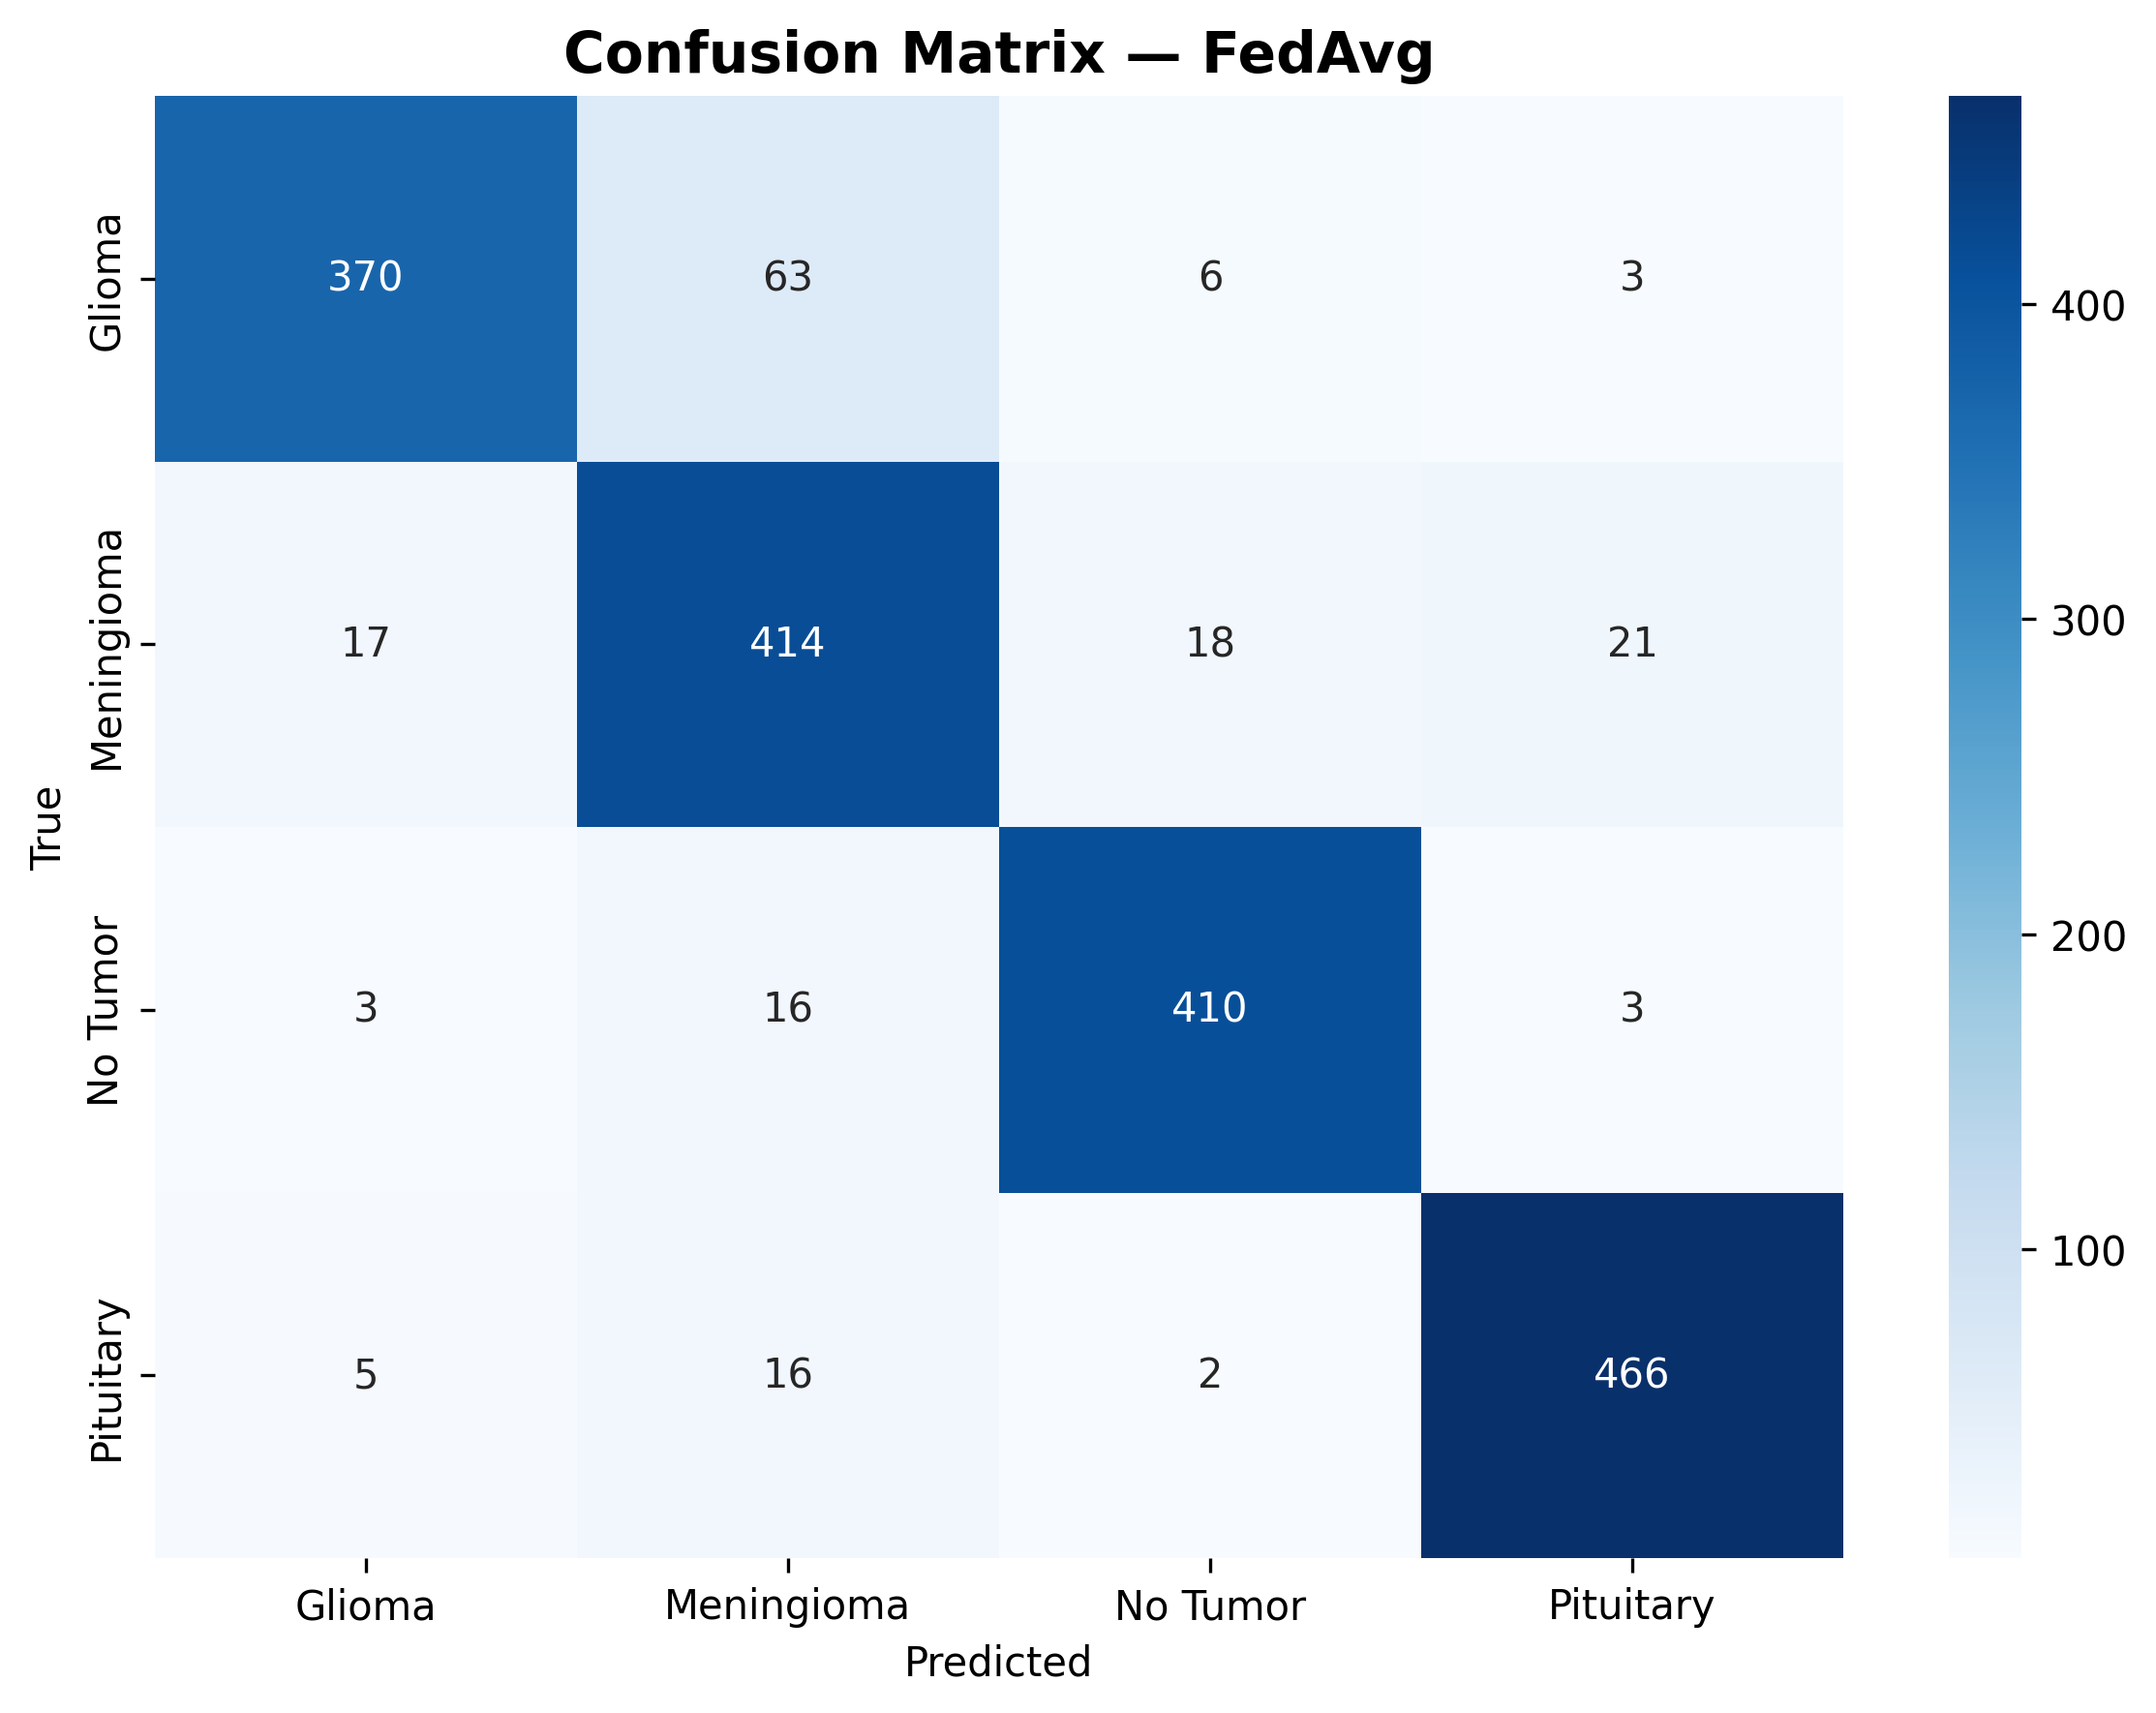
\includegraphics[width=0.48\columnwidth]{s1_cm_fedavg.png}%
  \hfill
  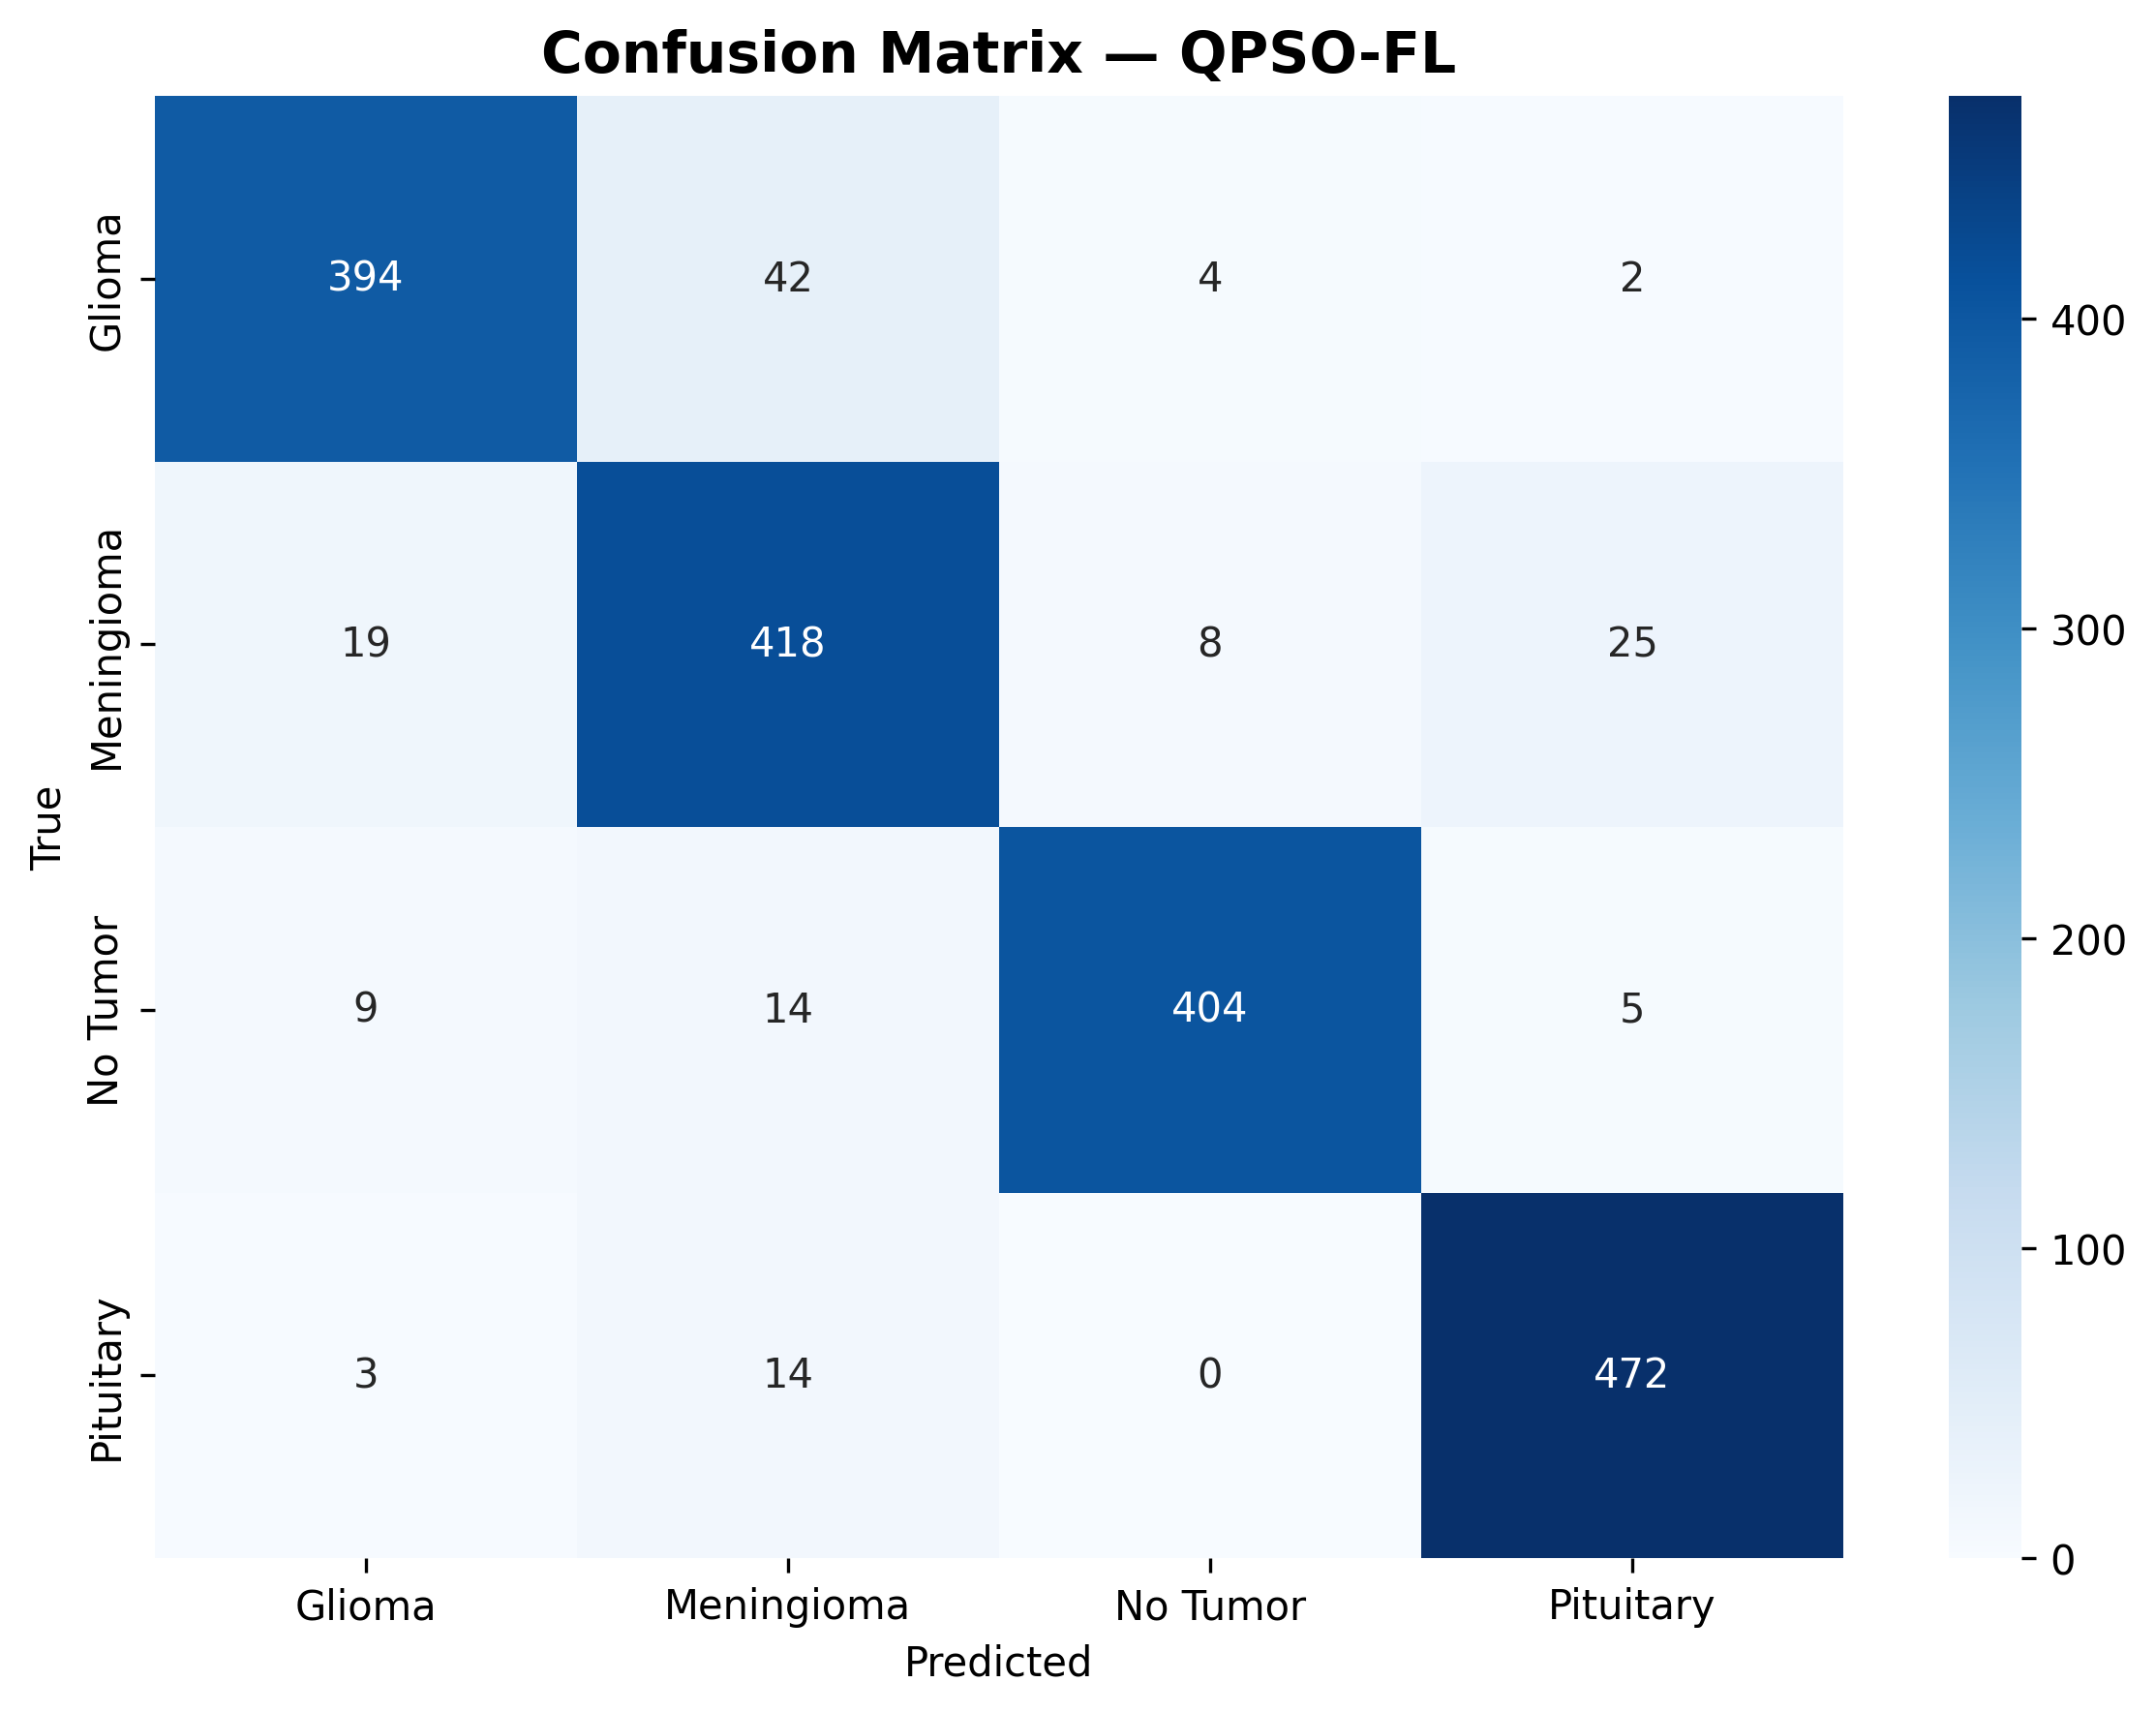
\includegraphics[width=0.48\columnwidth]{s1_cm_qpso.png}}
\caption{Confusion matrices --- Setup 1. Left: FedAvg. Right: FedQPSO. FedQPSO shows fewer Glioma misclassifications.}
\label{fig:cm_s1}
\end{figure}

\begin{figure}[t]
\centerline{%
  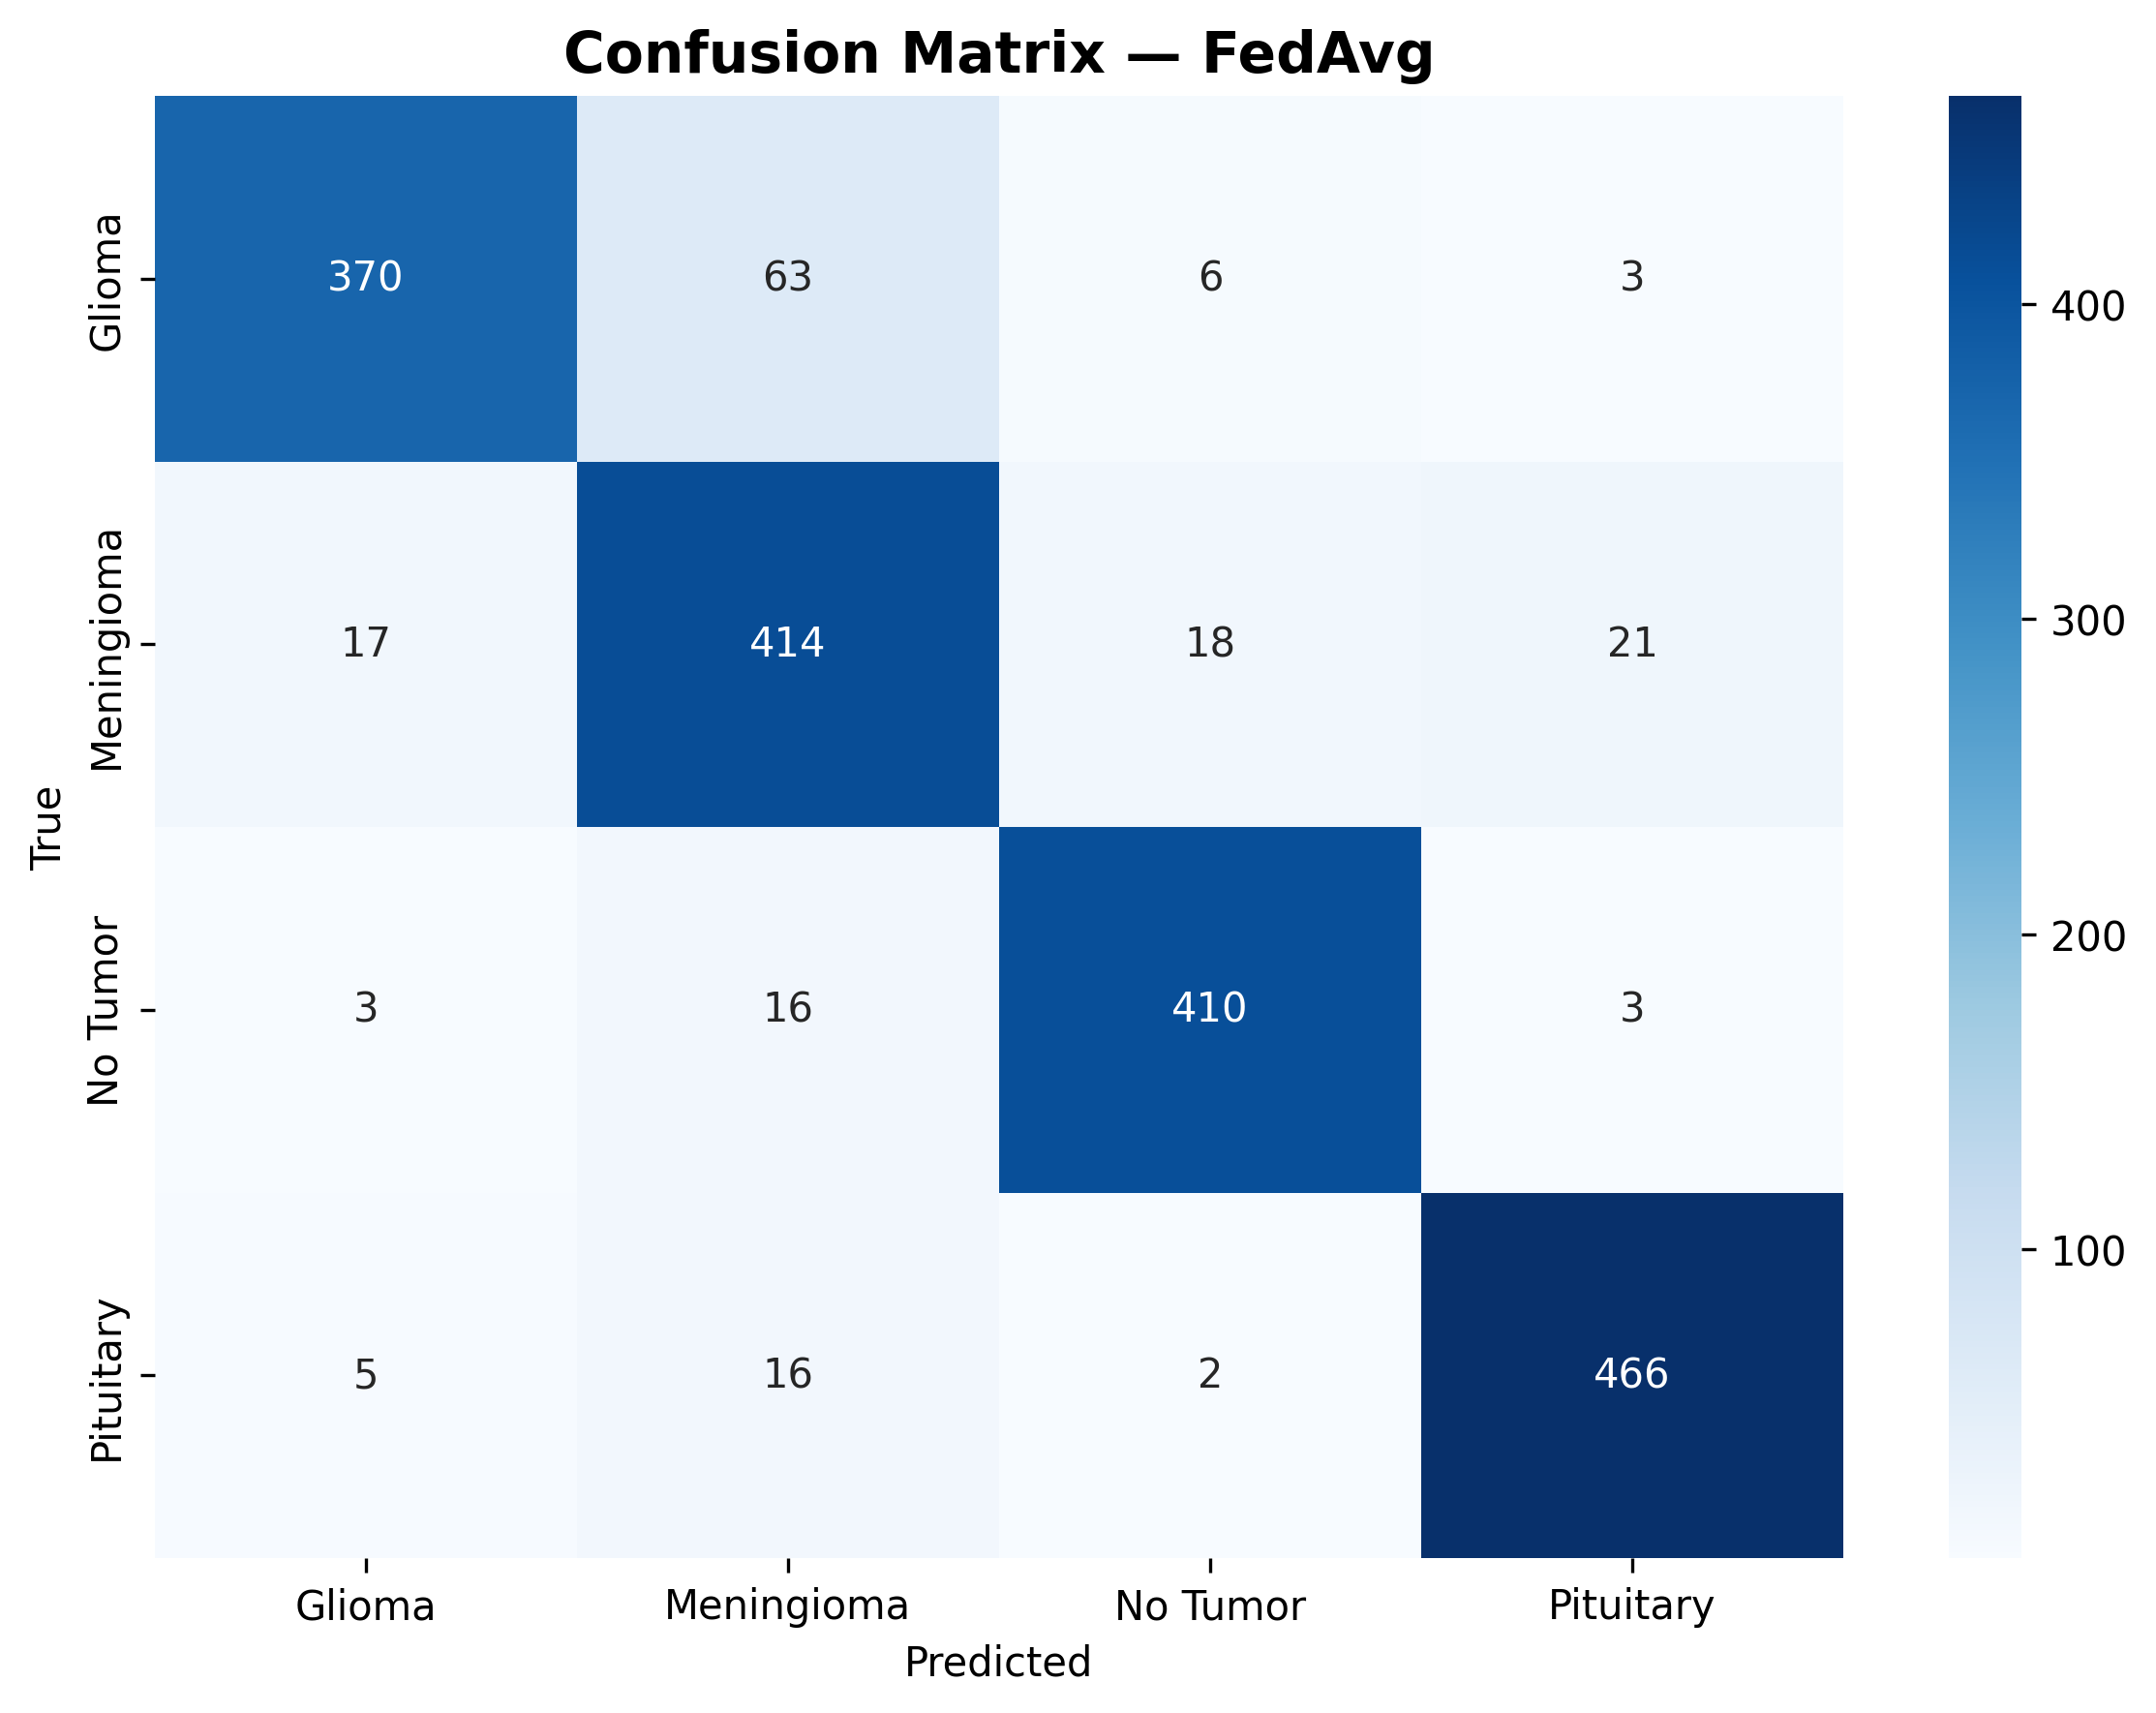
\includegraphics[width=0.48\columnwidth]{s2_cm_fedavg.png}%
  \hfill
  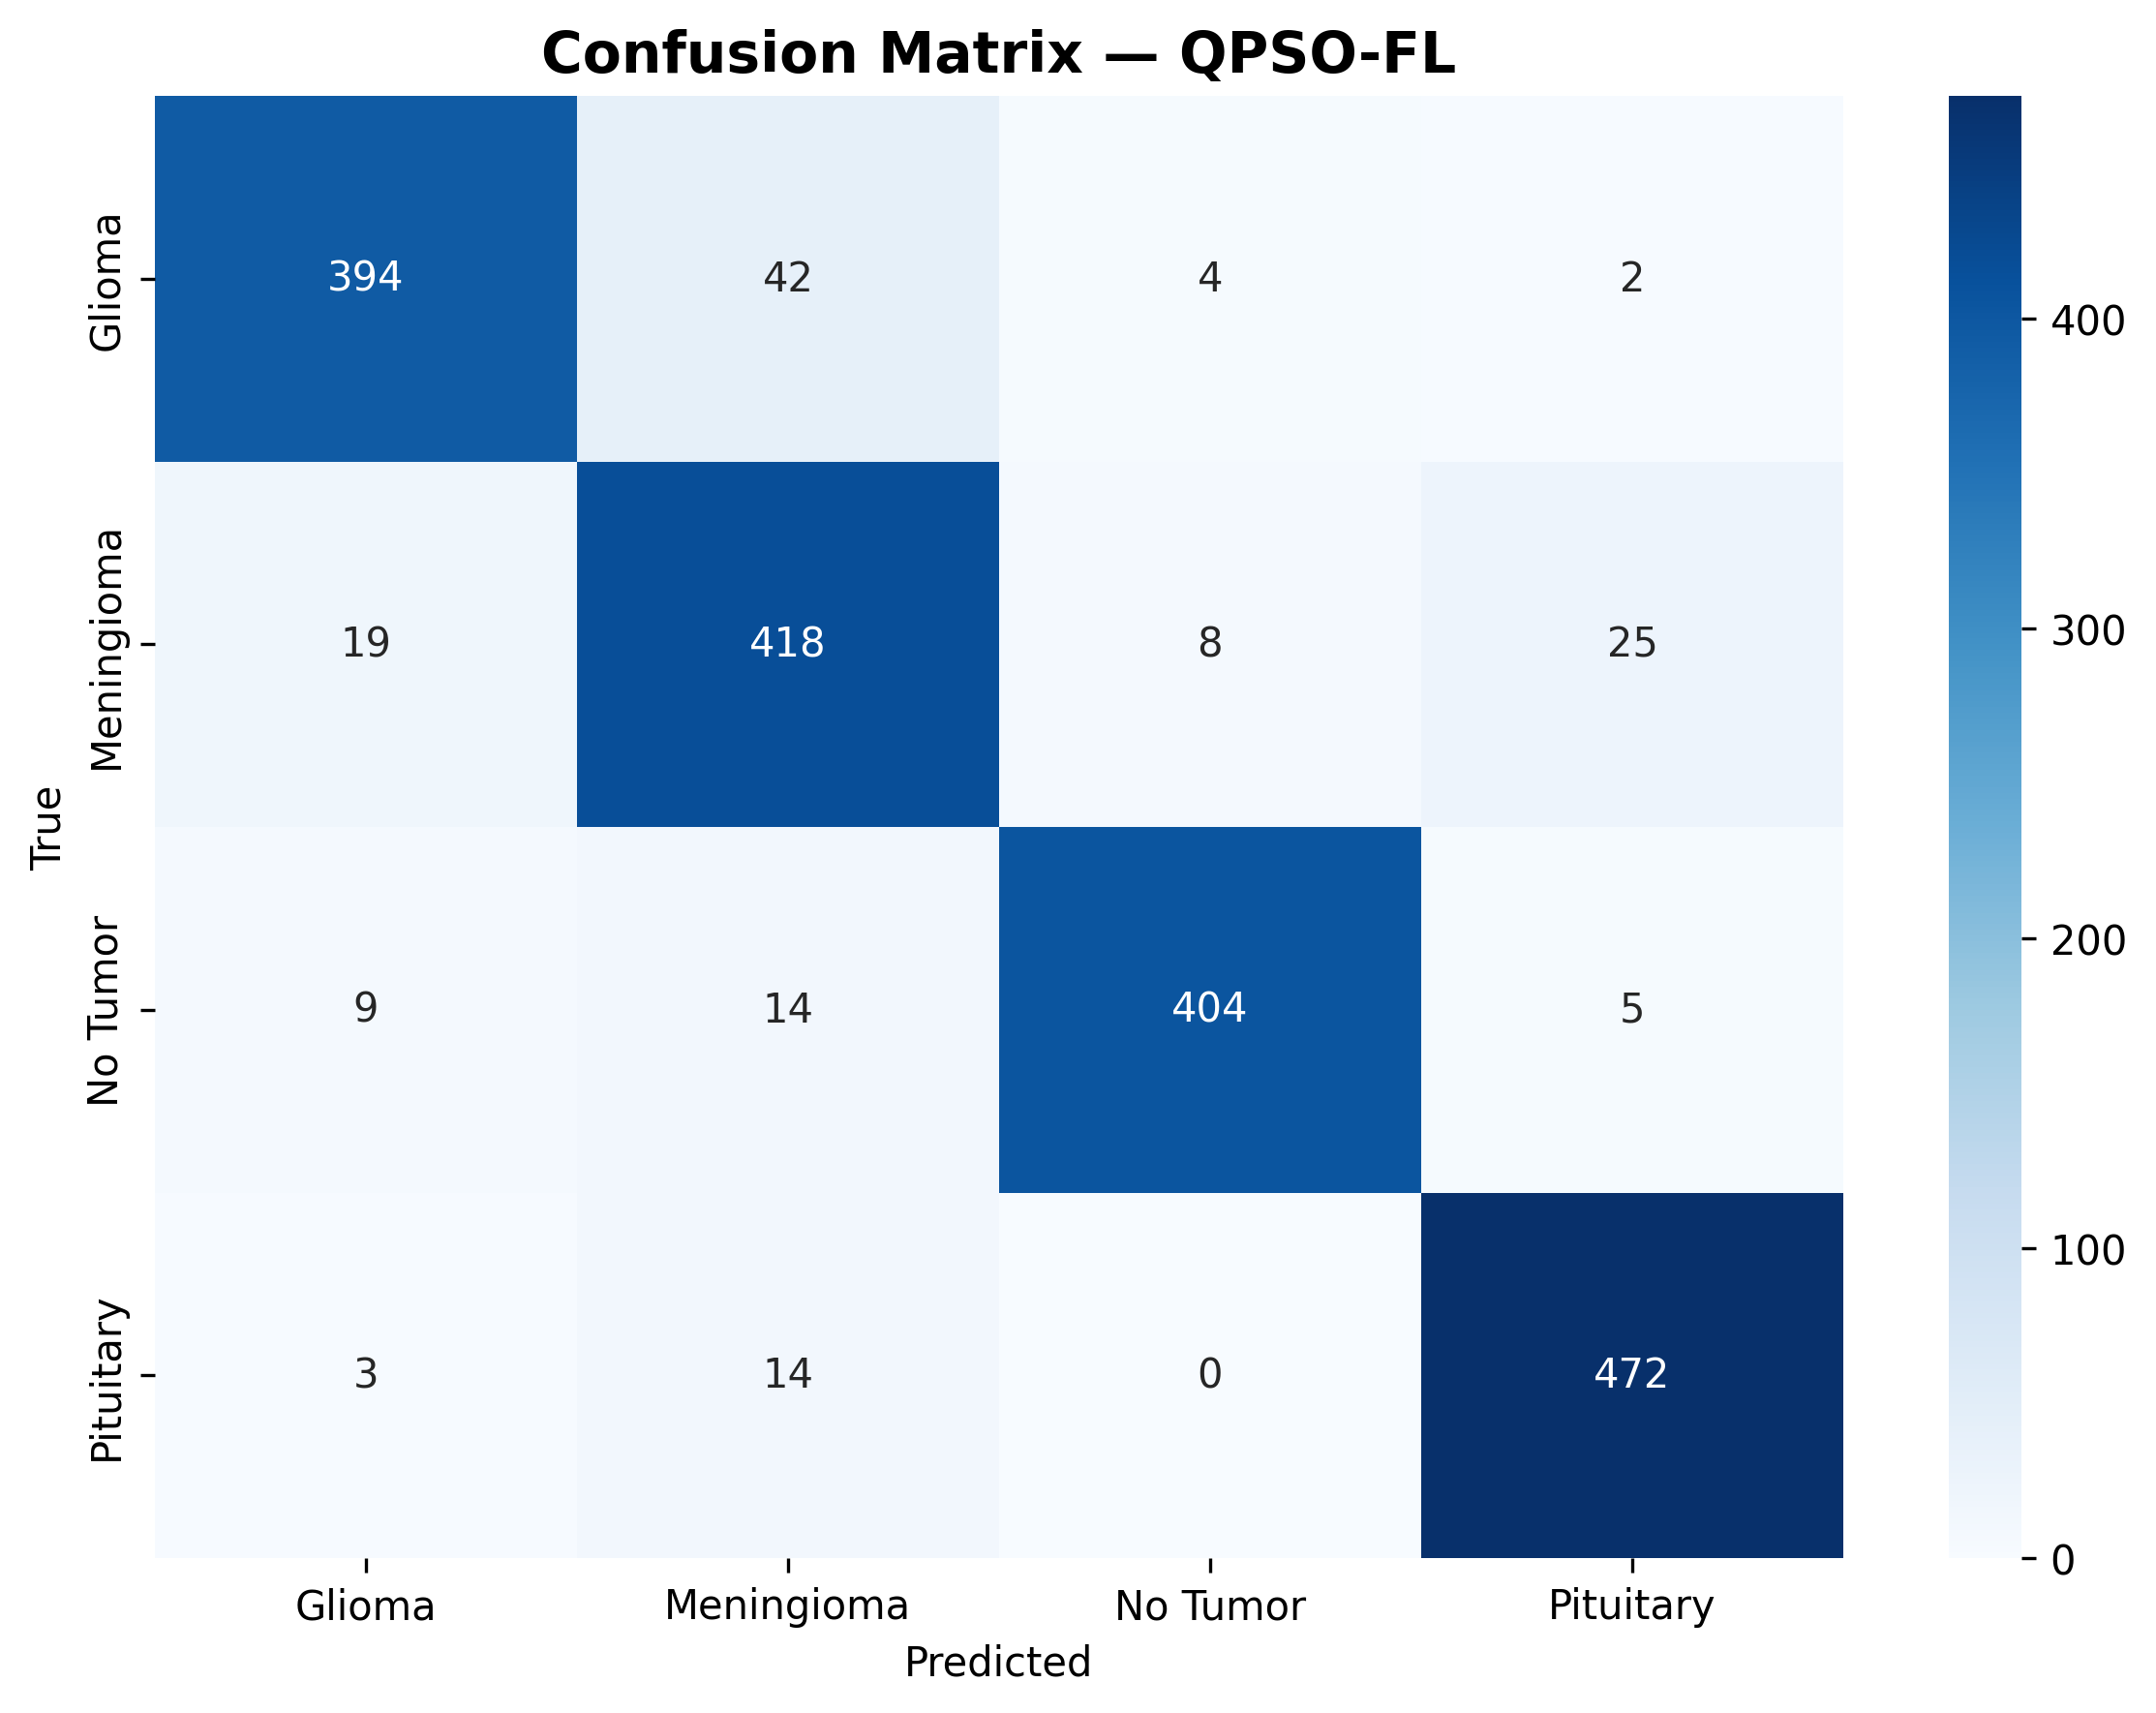
\includegraphics[width=0.48\columnwidth]{s2_cm_qpso.png}}
\caption{Confusion matrices --- Setup 2. Left: FedAvg. Right: FedQPSO. FedAvg shows Meningioma/Glioma confusions from label-skew bias.}
\label{fig:cm_s2}
\end{figure}

\subsection{Stability Analysis}

\begin{table}[t]
\caption{Accuracy Curve Stability}
\label{tab:stability}
\begin{center}
\begin{tabular}{llccc}
\hline
\textbf{Setup} & \textbf{Metric} & \textbf{FedAvg} & \textbf{FedProx} &
\textbf{FedQPSO}\\
\hline
\multirow{2}{*}{S1} & Max round drop (pp) & $-$11.51 & $-$8.46 &
\textbf{$-$2.45}\\
 & Round-to-round std (pp) & $\approx$4.0 & $\approx$4.0 & \textbf{2.22}\\
\hline
\multirow{2}{*}{S2} & Max round drop (pp) & $-$14.78 & $-$9.93 &
\textbf{$-$3.38}\\
 & Round-to-round std (pp) & 4.08 & 4.25 & \textbf{2.16}\\
\hline
\end{tabular}
\end{center}
\end{table}

As shown in Table~\ref{tab:stability}, FedQPSO's round-to-round volatility is
approximately \textbf{half} that of FedAvg and FedProx in both setups. The
largest drop across all 200 FedQPSO rounds (3.38 pp, Setup 2) is smaller than
FedAvg's single largest crash in the \emph{easier} natural heterogeneity
condition (11.51 pp). The fitness evaluation step prevents destabilizing weight
combinations from ever being committed to the global model.

% ============================================================
\section{Discussion}
\label{sec:discussion}
% ============================================================

\subsection{Why FedQPSO Is Fairer}
FedAvg's weighted average systematically over-represents large clients (Client
3 has 3.5$\times$ the data of Client 1, giving proportionally more influence
on every aggregated model). FedProx slows all clients equally but does not
redistribute influence. FedQPSO jointly optimizes each layer against a
\textbf{balanced combined validation set} from all three clients. A weight
configuration that performs well for Clients 2 and 3 but poorly for Client 1
yields high aggregate validation loss and is rejected. The fitness search
therefore naturally converges toward weights that minimize loss
\emph{simultaneously across all clients} --- an implicit fairness constraint
requiring no explicit fairness regularizer.

\subsection{The Role of Algorithm Design: Naive vs.\ Layer-by-Layer QPSO}
Our Phase~3 experiments with a naive whole-model QPSO (blind perturbation of
all 120K parameters simultaneously, no fitness evaluation) produced
catastrophic results: 77.3\% accuracy under label skew versus FedAvg's
90.56\% --- a 13.26 pp deficit. The layer-by-layer redesign with
validation-loss fitness evaluation recovered 14.79 pp and exceeded FedAvg in
both setups. The critical difference: without evaluating the result of
perturbation, QPSO is indistinguishable from deliberate noise injection. With
fitness evaluation, it becomes a genuine optimization procedure.

\subsection{Global Accuracy as a Misleading Metric}
When FedAvg achieved its peak global accuracy of 90.56\% (Setup 2), Client 1
was simultaneously at 52.92\% --- barely above chance. Under FedQPSO, the same
client was at 80.83\% at FedQPSO's own peak of 92.09\%. Global test accuracy
measured on a balanced combined test set \emph{actively hides} severe
per-client disparities. In healthcare, this inequity is not a statistical
artifact --- it represents patients at smaller hospitals receiving substantially
inferior diagnostic support. We recommend that future FL medical imaging work
\emph{always} report per-client performance alongside global metrics.

\subsection{Clinical Interpretation}
FedQPSO is the \textbf{only} tested algorithm that keeps the weakest client
above 80\% accuracy at convergence under label skew. Its superior Glioma
recall (0.8914 vs.\ 0.8620 for FedProx, 0.8371 for FedAvg under Setup 2)
translates to fewer missed glioma diagnoses. The stability advantage (max
crash $\leq$3.38 pp vs.\ $\leq$14.78 pp for FedAvg) is also clinically
meaningful: a sudden 15 pp degradation in model performance during a deployed
FL round would provide dangerously unreliable diagnostic support until the
next stable round.

\subsection{Computational Trade-offs}
FedQPSO's 9.4$\times$ compute overhead relative to FedAvg (approximately 125
minutes vs.\ 13 minutes for 100 rounds on a P100 GPU) is its only
unambiguous disadvantage. Crucially, this overhead is borne \emph{entirely by
the central server} --- participating hospitals experience identical local
training costs. In offline model development contexts, 2 hours of total
training time is entirely practical. For high-frequency real-time retraining
deployments, the overhead may need to be mitigated through reduced QPSO
iterations or selective layer application.

% ============================================================
\section{Limitations and Future Work}
\label{sec:limitations}
% ============================================================

\textbf{Computational cost:} 9.4$\times$ overhead limits retraining frequency.
Future work should explore reducing $T$ or applying FedQPSO selectively to
high-variance layers only.

\textbf{Client scale:} Only 3 clients were evaluated. Fairness claims should
be validated with 5--10 clients simulating more diverse institutional
configurations and data heterogeneity profiles.

\textbf{Architecture:} SimpleCNN was chosen to isolate aggregation as the
performance variable. It would be valuable to evaluate FedQPSO with deeper
(EfficientNet-B0, MobileNetV3) and pretrained architectures, with appropriate
controls for confounding factors.

\textbf{QPSO hyperparameters:} $\beta = 0.6$ and $T = 5$ were adopted from
the MNIST reference \cite{edla2025mnist} without task-specific tuning.
Sensitivity analyses and adaptive scheduling of $\beta$ may improve results.

\textbf{Single seed:} Run-to-run variance across multiple random seeds was not
measured. Future work should report confidence intervals.

\textbf{Privacy guarantees:} Only structural privacy via FL is provided. Adding
formal differential privacy guarantees (e.g.\ Gaussian gradient noise) may
reduce accuracy but would strengthen privacy claims.

% ============================================================
\section{Conclusion}
\label{sec:conclusion}
% ============================================================

We introduced \textbf{FedQPSO}, a novel federated aggregation algorithm
applying layer-by-layer Quantum Particle Swarm Optimization with
validation-loss fitness evaluation to the problem of equitable brain tumor MRI
classification across heterogeneous clinical sites. Through a four-phase
experimental progression on real-world MRI data, we demonstrated that:

\begin{itemize}
    \item FedQPSO reduces the inter-client performance gap by 72--81\% compared
    to FedAvg, and by 45--56\% compared to FedProx.
    \item FedQPSO is the only method maintaining clinically useful accuracy
    ($\geq$80\%) at the weakest client under label skew.
    \item FedQPSO achieves the highest Glioma recall in both experimental
    conditions and demonstrates the most stable accuracy trajectories.
    \item FedQPSO's statistical advantage over FedAvg scales with heterogeneity
    severity (Cohen's $d$: $0.35 \to 1.26$).
    \item The fairness benefit arises from an implicit mechanism: combined
    cross-client validation fitness evaluation, requiring no explicit fairness
    objective.
\end{itemize}

These results establish FedQPSO as the preferred aggregation strategy for
fairness-critical federated deployments in multi-institutional medical imaging
when client equity is a primary objective and the 9$\times$ compute overhead
is acceptable.

% ============================================================
\section*{Acknowledgment}
The authors acknowledge the support of the Department of Computer Science \&
Engineering, Matrusri Engineering College. Compute resources were provided via
Kaggle's GPU platform (Tesla P100-16GB). The Masoud Brain Tumor MRI dataset
and the BRISC 2025 dataset, both publicly available on Kaggle, are gratefully
acknowledged.

% ============================================================
\begin{thebibliography}{00}

\bibitem{mcmahan2017}
H.~B. McMahan, E.~Moore, D.~Ramage, S.~Hampson, and B.~A. y~Arcas,
``Communication-efficient learning of deep networks from decentralized data,''
in \textit{Proc.\ 20th Int.\ Conf.\ Artif.\ Intell.\ Stat.\ (AISTATS)},
Fort Lauderdale, FL, USA, Apr.\ 2017, pp.~1273--1282.

\bibitem{li2020fedprox}
T.~Li, A.~K. Sahu, M.~Zaheer, M.~Sanjabi, A.~Smola, and V.~Smith,
``Federated optimization in heterogeneous networks,''
in \textit{Proc.\ 3rd Conf.\ Mach.\ Learn.\ Syst.\ (MLSys)}, Austin, TX, USA,
Mar.\ 2020, pp.~429--450.

\bibitem{karimireddy2020scaffold}
S.~P. Karimireddy, S.~Kale, M.~Mohri, S.~Reddi, S.~Stich, and A.~T. Suresh,
``SCAFFOLD: Stochastic controlled averaging for federated learning,''
in \textit{Proc.\ 37th Int.\ Conf.\ Mach.\ Learn.\ (ICML)}, Vienna, Austria,
Jul.\ 2020, pp.~5132--5143.

\bibitem{zhao2018}
J.~Zhao, M.~Li, J.~Xu, and W.~Li,
``Federated learning with non-IID data,''
\textit{arXiv:1806.00582}, Jun.\ 2018.

\bibitem{sun2004qpso}
J.~Sun, B.~Feng, and W.~Xu,
``Particle swarm optimization with particles having quantum behavior,''
in \textit{Proc.\ 2004 Congr.\ Evol.\ Comput.\ (CEC)}, Portland, OR, USA,
Jun.\ 2004, vol.~1, pp.~325--331.

\bibitem{sheller2018}
M.~J. Sheller, G.~A. Reina, B.~Edwards, J.~Martin, and S.~Bakas,
``Multi-institutional deep learning modeling without sharing patient data:
A feasibility study on brain tumor segmentation,''
in \textit{Proc.\ Int.\ MICCAI Brainlesion Workshop}, Granada, Spain,
Sep.\ 2018, pp.~92--104.

\bibitem{rieke2020}
N.~Rieke \textit{et al.},
``The future of digital health with federated learning,''
\textit{npj Digit.\ Med.}, vol.~3, no.~1, pp.~1--7, Sep.\ 2020.

\bibitem{sultan2019}
H.~H. Sultan, N.~M. Salem, and W.~Al-Atabany,
``Multi-classification of brain tumor images using deep neural network,''
\textit{IEEE Access}, vol.~7, pp.~69 215--69 225, 2019.

\bibitem{ostrom2021}
Q.~T. Ostrom \textit{et al.},
``CBTRUS statistical report: Primary brain and other central nervous system
tumors diagnosed in the United States in 2014--2018,''
\textit{Neuro-oncology}, vol.~23, no.~suppl\_3, pp.~iii1--iii105, 2021.

\bibitem{hipaa}
U.S.\ Department of Health \& Human Services,
``Health Insurance Portability and Accountability Act (HIPAA) of 1996,''
Public Law 104-191, 1996.

\bibitem{kennedy1995}
J.~Kennedy and R.~Eberhart,
``Particle swarm optimization,''
in \textit{Proc.\ ICNN'95 --- Int.\ Conf.\ Neural Netw.}, Perth, WA, Australia,
Nov.--Dec.\ 1995, vol.~4, pp.~1942--1948.

\bibitem{fedpso2021}
J.~Park, H.~J. Kim, and J.~Moon,
``FedPSO: Federated learning using particle swarm optimization to
reduce communication costs,''
\textit{Sensors}, vol.~21, no.~2, p.~600, Jan.\ 2021.

\bibitem{kulkarni2020pfl}
V.~Kulkarni, M.~Kulkarni, and A.~Pant,
``Survey of personalization techniques for federated learning,''
in \textit{Proc.\ 2020 4th World Conf.\ Smart Trends Syst., Secur. Sustainability},
London, UK, Jul.\ 2020, pp.~794--797.

\bibitem{masoud}
M. Nickparvar,
``Brain tumor MRI dataset,''
Kaggle, 2021. [Online]. Available:
\url{https://www.kaggle.com/datasets/masoudnickparvar/brain-tumor-mri-dataset}

\bibitem{brisc}
BRISC Dataset Contributors,
``BRISC 2025 brain tumor classification dataset,''
Kaggle, 2025. [Online]. Available:
\url{https://www.kaggle.com/datasets/briscdataset/}

\bibitem{edla2025mnist}
Divyansh Teja Edla,
``Enhancing federated learning with quantum-inspired particle swarm
optimization: An {IID} {MNIST} study,'' (Paper ID: CSE-104)
in \textit{Proc.\ AICTE Sponsored Natl.\ Conf.\ Innovations, Challenges
and Solutions in Eng., Sci.\ and Technol.\ (NCICSET'25)},
Sri Indu College of Engineering and Technology, Hyderabad, India,
Dec.\ 17--18, 2025.

\end{thebibliography}

\end{document}

